\chapter{Event Selection}
\label{event_selection_chapter}

In this chapter we discuss the acceptance region for this analysis, as well as
how events are selected for the analysis. Additionally, we discuss the
background that makes it through the selection process, and the method in which
we correct for selection and detector effects through unfolding.

\section{Acceptance}
\label{sec:acceptance}

The acceptance region is a definition of what events, assuming that there are
no limitations due to the detector design, are include in the analysis. The
acceptance region is what the final result of this analysis will be corrected
to, ensuring that other measurements and theoretical predictions can be
compared to our results without having to account for the detector response.
The acceptance region defines what sort of physics results we can make
statements about, and also determines the value of the effective cross section
of the \Z.

Our acceptance is defined by the kinematics of the two electrons and the mass
of the Z boson. One of the electrons, called the \CentralElectron, is required
to have $\pt > 30 \GeV$ and to be within the central region of the detector
(hence the name) with $|\eta| < 2.1$. The other electron, called the
\ExtendedElectron, has looser requirements; it must have $\pt > 20 \GeV$ and is
not required to be as central with $|\eta| < 2.4$. The requirements on the
\CentralElectron were selected in conjunction with the \Ztomumu measurement of
\phistar at CMS so that that measurement and this one could be easily combined
into a joint measurement. The pseudorapidity limit was selected to match the
most efficient region of CMS's single muon trigger, while the transverse
momentum threshold was dictated by threshold on single electron trigger. The
pseudorapidity limit on the \ExtendedElectron was chosen to keep all of the
electrons within the region covered by the tracker (which allows a better
angular measurement than ECAL alone), while the transverse momentum threshold
was selected because for $\pt < 20 \GeV$ the rate of fake electrons increases.

There are other particles, like the \jpsi, that decay to \ee pairs as shown in
\FIG~\ref{fig:ee_spectrum}. Fortunately, none of these other particles are near
the \Z in mass, and so we can eliminate them from our acceptance by requiring a
mass near the \Z peak. We therefore define our mass window around the nominal
\Z mass of $91 \GeV$, extending from $60 \GeV$ to $120 \GeV$.

\begin{figure}[!htbp]
    \centering
    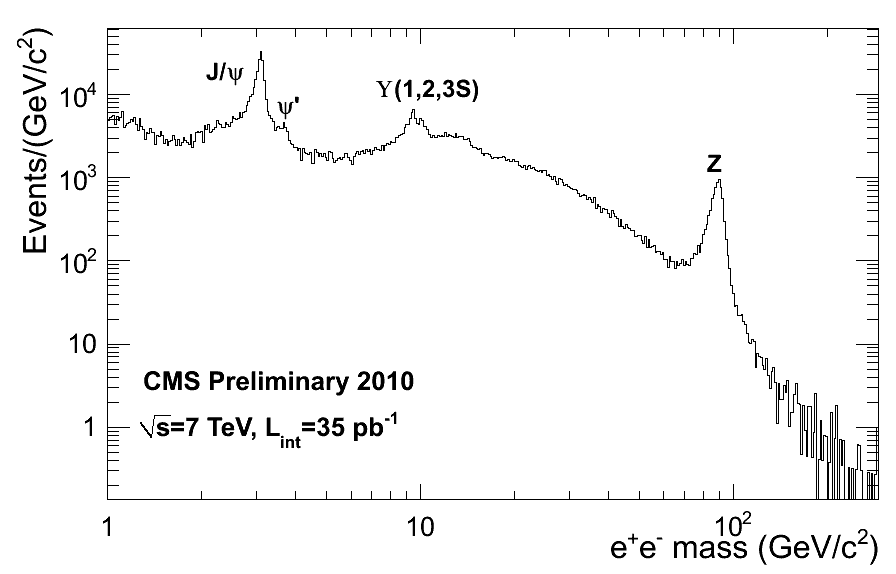
\includegraphics[width=\textwidth]{figures/dielectron_mass_7tev.png}
    \caption{
        The spectrum of \ee events as measured by CMS in 2010.
    }
    \label{fig:ee_spectrum}
\end{figure}

\section{Object Selection}

\subsection{Electron Selection}
\label{ssec:electron_selection}

The requirements used to select electrons are chosen to be tighter than the
requirements used at the trigger level in order to make calculating the various
efficiencies easier. For an event to be considered it must have at least two
electrons that pass the acceptance requirements for \ExtendedElectrons: $\pt >
20 \GeV$ and $|\eta| < 2.4$. If three or more electrons pass this initial
requirement, only the two with the highest \pt are considered. One of these two
electrons must be within $|\eta| < 2.1$ and it must also have $\pt > 30 \GeV$.

A \CentralElectron in the event is required to pass \EGTIGHT and to be matched
to one of the electrons that passed \SingleElectronTrigger with $\Delta R <
0.3$. The other electron must pass \EGMEDIUM. If both electrons are
\CentralElectrons, then only one of them need pass \EGTIGHT, but this same
electron must also match the trigger; the other \CentralElectron need only pass
\EGMEDIUM. The definitions of \EGMEDIUM and \EGTIGHT are discussed in
\SEC~\ref{sec:cut_based_id}.

No charge requirement is applied because the number of signal events removed by
this selection is larger than the number of background events supressed.

The distributions of electron \pt and $\eta$ for the highest \pt electron and
the second highest \pt electron after all selection requirements are applied
are shown in \FIGS~\ref{fig:e_pt} and \ref{fig:e_eta}.

\begin{figure}[!htbp]
    \centering
    \begin{subfigure}[b]{0.65\textwidth}
        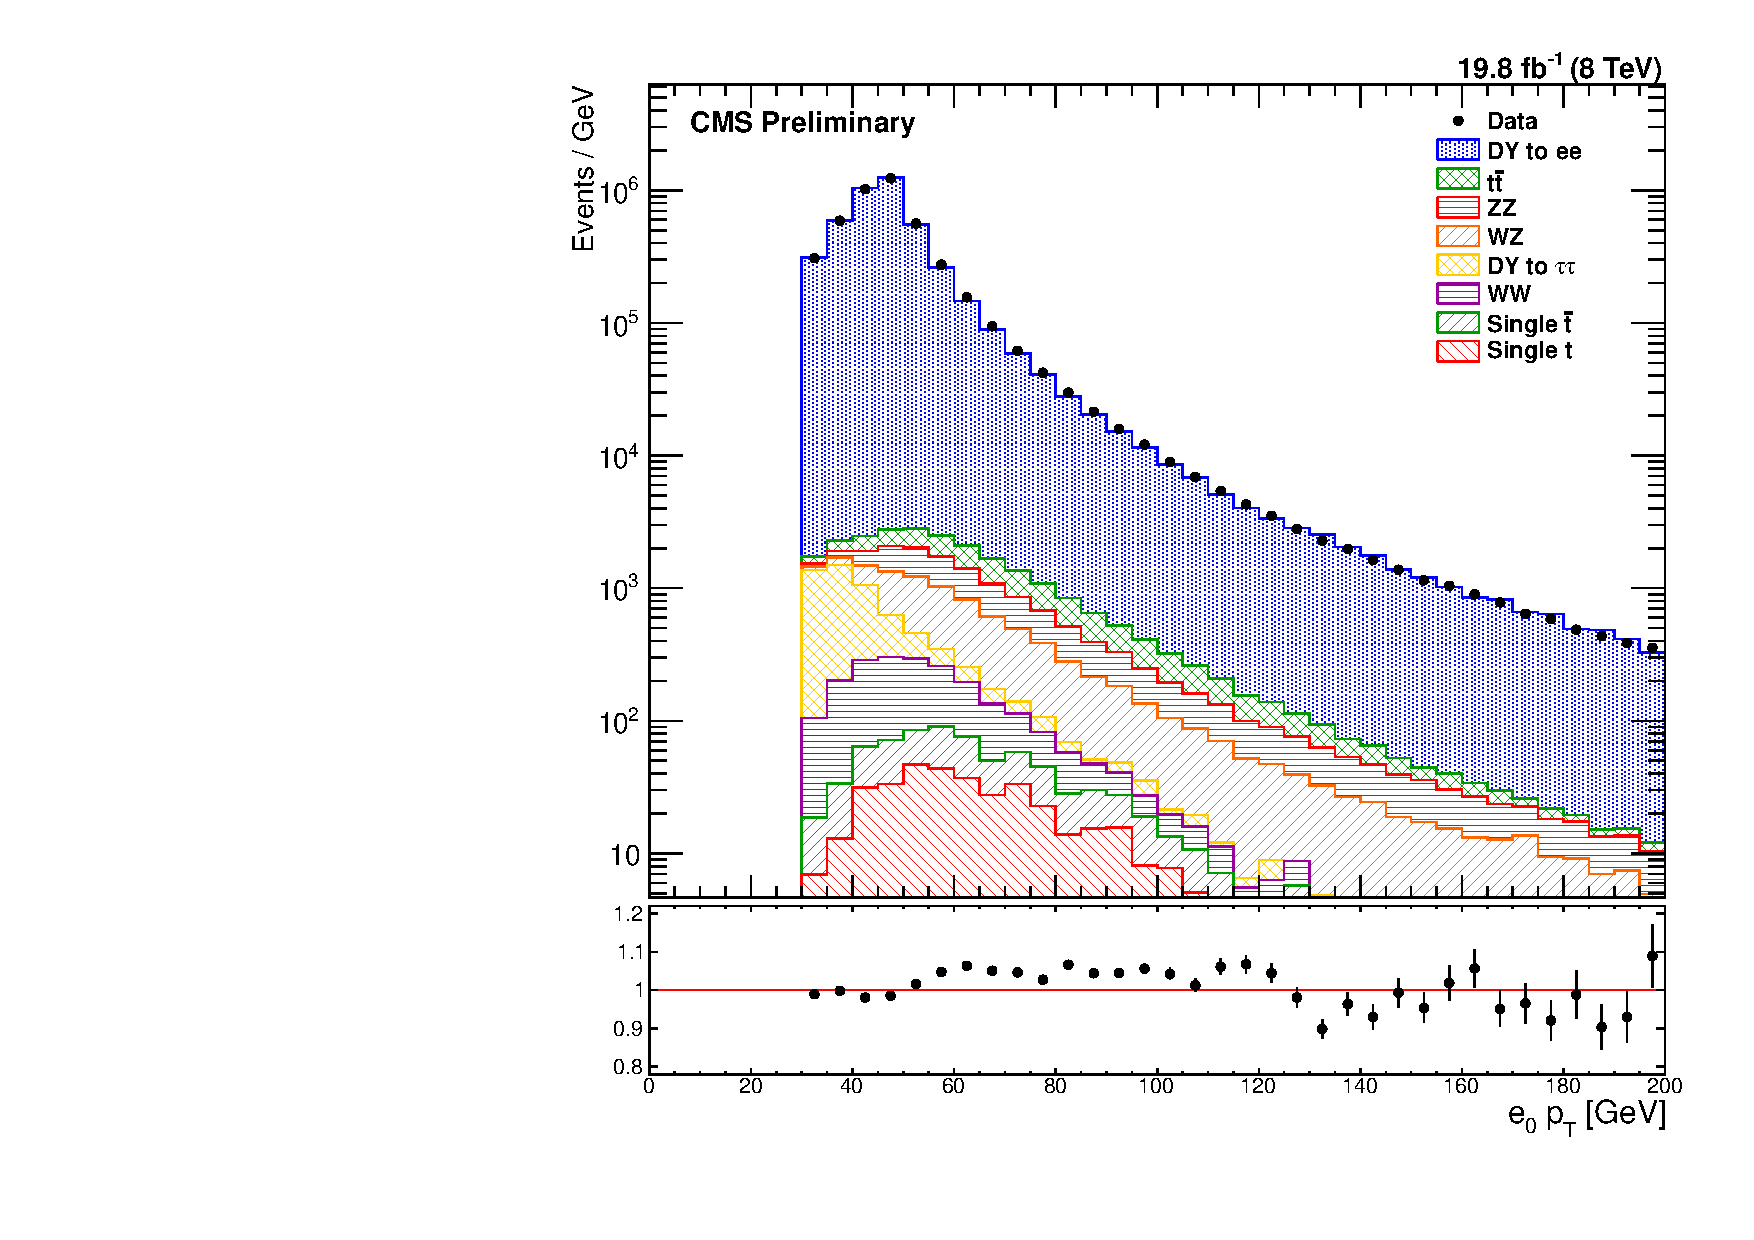
\includegraphics[width=\textwidth]{figures/e0_pt.pdf}
        \caption{}
        \label{fig:e_pt_high}
    \end{subfigure}
    \begin{subfigure}[b]{0.65\textwidth}
        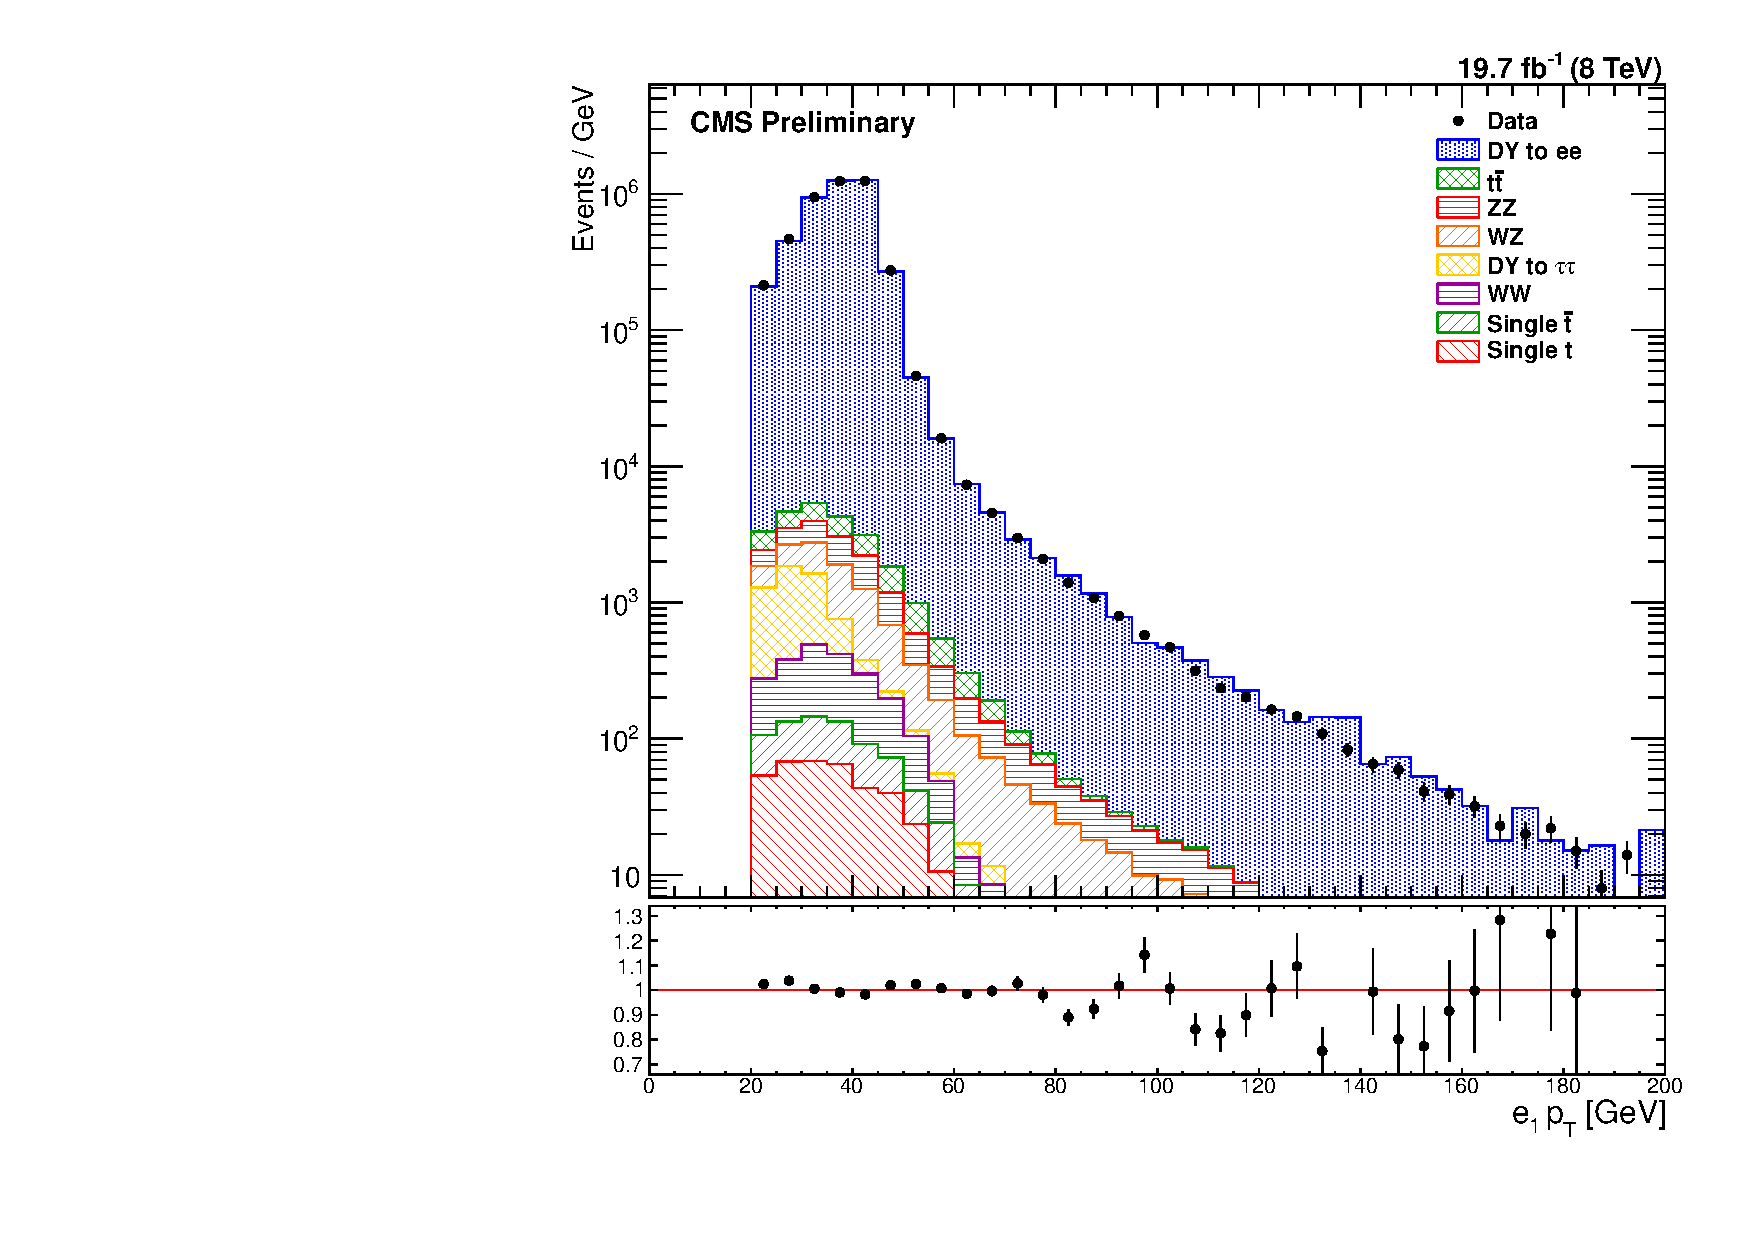
\includegraphics[width=\textwidth]{figures/e1_pt.pdf}
        \caption{}
        \label{fig:e_pt_low}
    \end{subfigure}
    \caption[
        The \pt distribution of electrons in data.
    ]{
        The \pt distribution of the higher (top) and lower (bottom) \pt
        electrons in data (points) and \MADGRAPH signal MC and the background
        MC samples (histograms) for events passing the full analysis selection.
    }
    \label{fig:e_pt}
\end{figure}

\begin{figure}[!htbp]
    \vspace*{\fill}
    \centering
    \begin{subfigure}[b]{0.65\textwidth}
        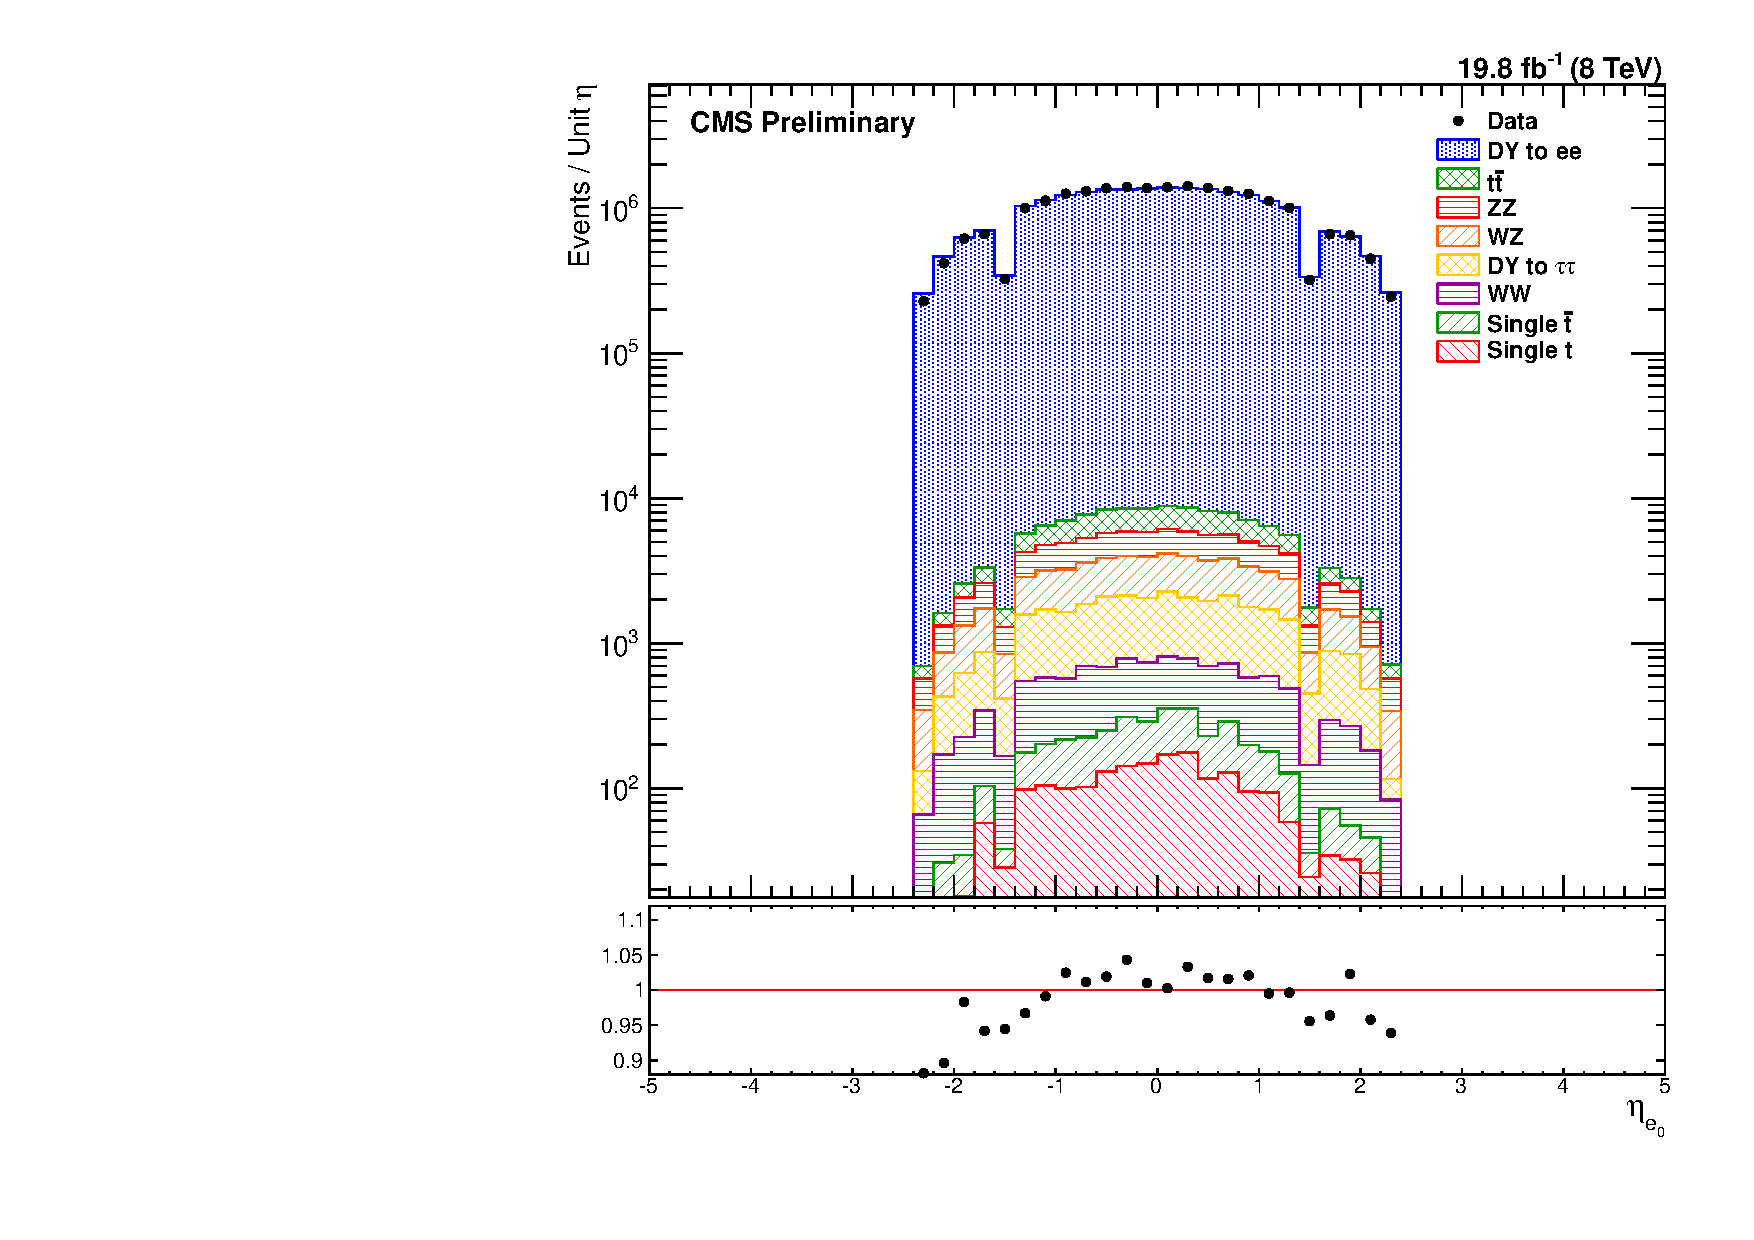
\includegraphics[width=\textwidth]{figures/e0_eta.pdf}
        \caption{}
        \label{fig:e_eta_high}
    \end{subfigure}
    \begin{subfigure}[b]{0.65\textwidth}
        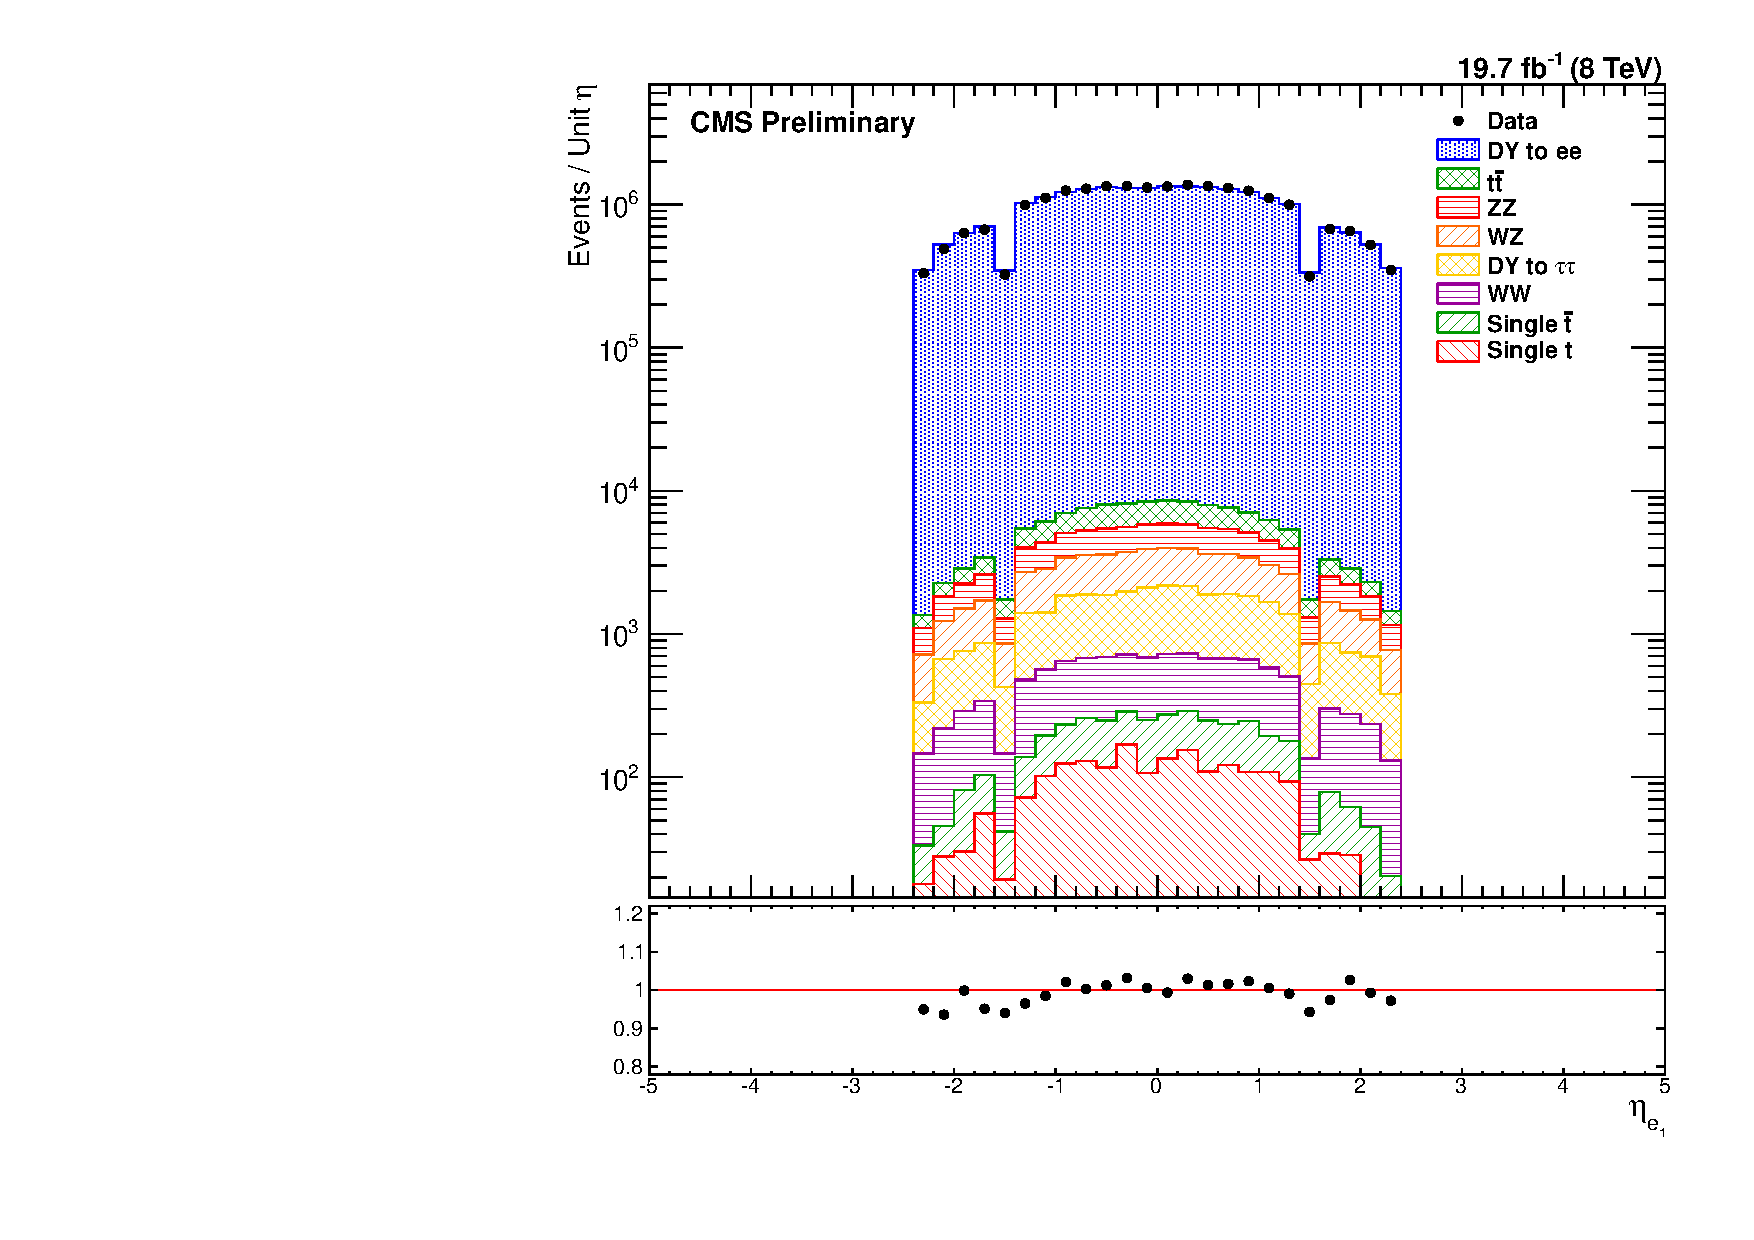
\includegraphics[width=\textwidth]{figures/e1_eta.pdf}
        \caption{}
        \label{fig:e_eta_low}
    \end{subfigure}
    \caption[
        The $\eta$ distribution of electrons in data.
    ]{
        The $\eta$ distribution of the higher (top) and lower (bottom) \pt
        electrons in data (points) and \MADGRAPH signal MC and the background
        MC samples (histograms) for events passing the full analysis selection.
    }
    \label{fig:e_eta}
\end{figure}

\subsection{\Z Selection}

The \Z boson decays too quickly to leave any direct signal in the detector, so
it is reconstructed from its decay products: the two electrons whose selection
is described in \SEC~\ref{ssec:electron_selection}. In events where the two
electrons pass the selection, the \Z is constructed by taking the sum of the
electrons four-vectors. The resulting invariant mass of the \Z must be within
the region set by the acceptance (\MassRange).

The distributions of \mee, \Z \pt, and \Z \rapidity after these selection
requirements are applied are shown with \MADGRAPH signal MC in
\FIGS~\ref{fig:z_mass}, \ref{fig:z_pt}, and \ref{fig:z_rapidity}, and with
\POWHEG signal MC in \FIGS~\ref{fig:z_mass_powheg}, \ref{fig:z_pt_powheg}, and
\ref{fig:z_rapidity_powheg}. It is worth noting that \MADGRAPH poorly
approximates the \rapidity distribution found in data, but that \POWHEG does
relatively worse in approximating the \pt distribution. Both samples do a
comparable job of approximating the \mee distribution in data. \TODO{Should I
show the lepton \pt plots, where \MADGRAPH is much better?}

\begin{figure}[!htbp]
    \centering
    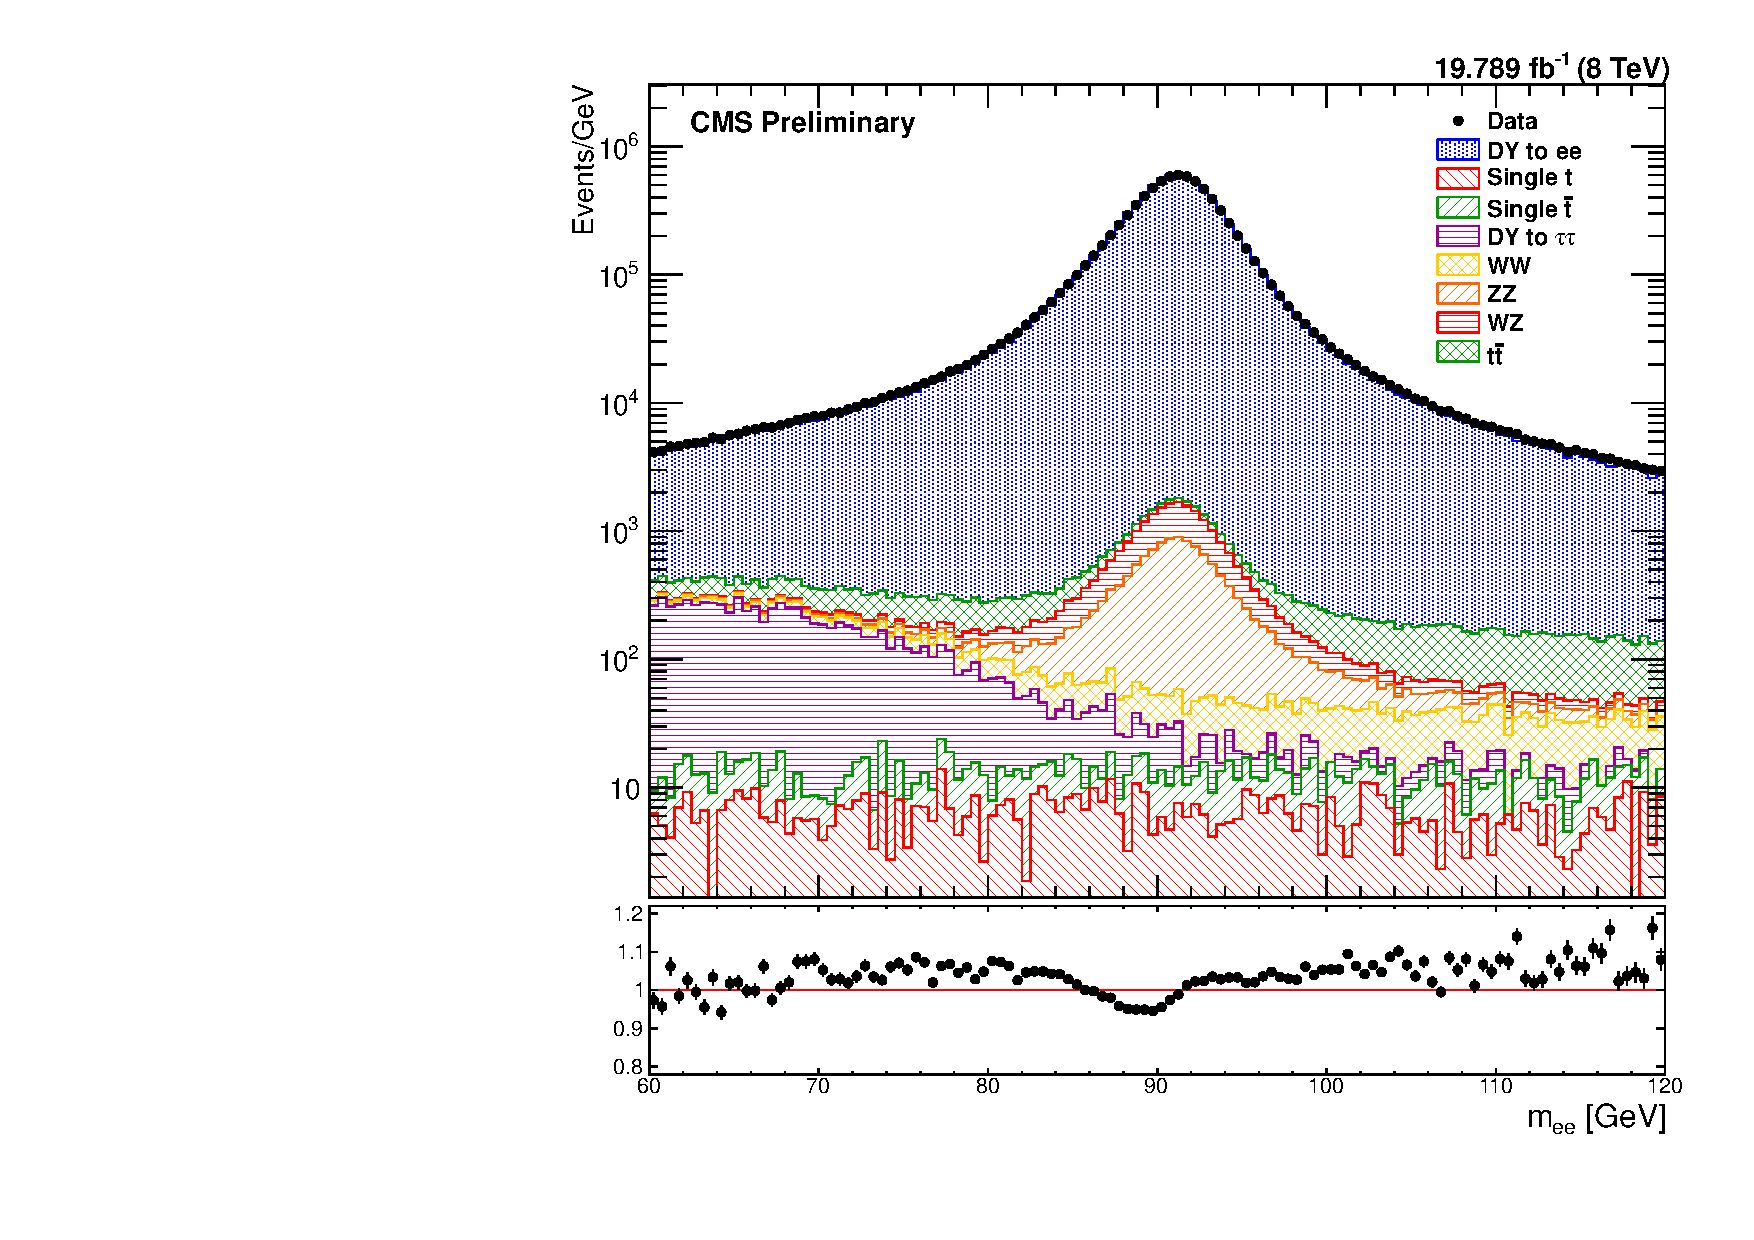
\includegraphics[width=\textwidth]{figures/z_mass_fine.pdf}
    \caption[
        The \mee distribution of events in data and MC with \MADGRAPH signal MC.
    ]{
        The \mee distribution of all events passing the final selection in data
        (points) and \MADGRAPH signal MC and the background MC samples
        (histograms).
    }
    \label{fig:z_mass}
\end{figure}

\begin{figure}[!htbp]
    \centering
    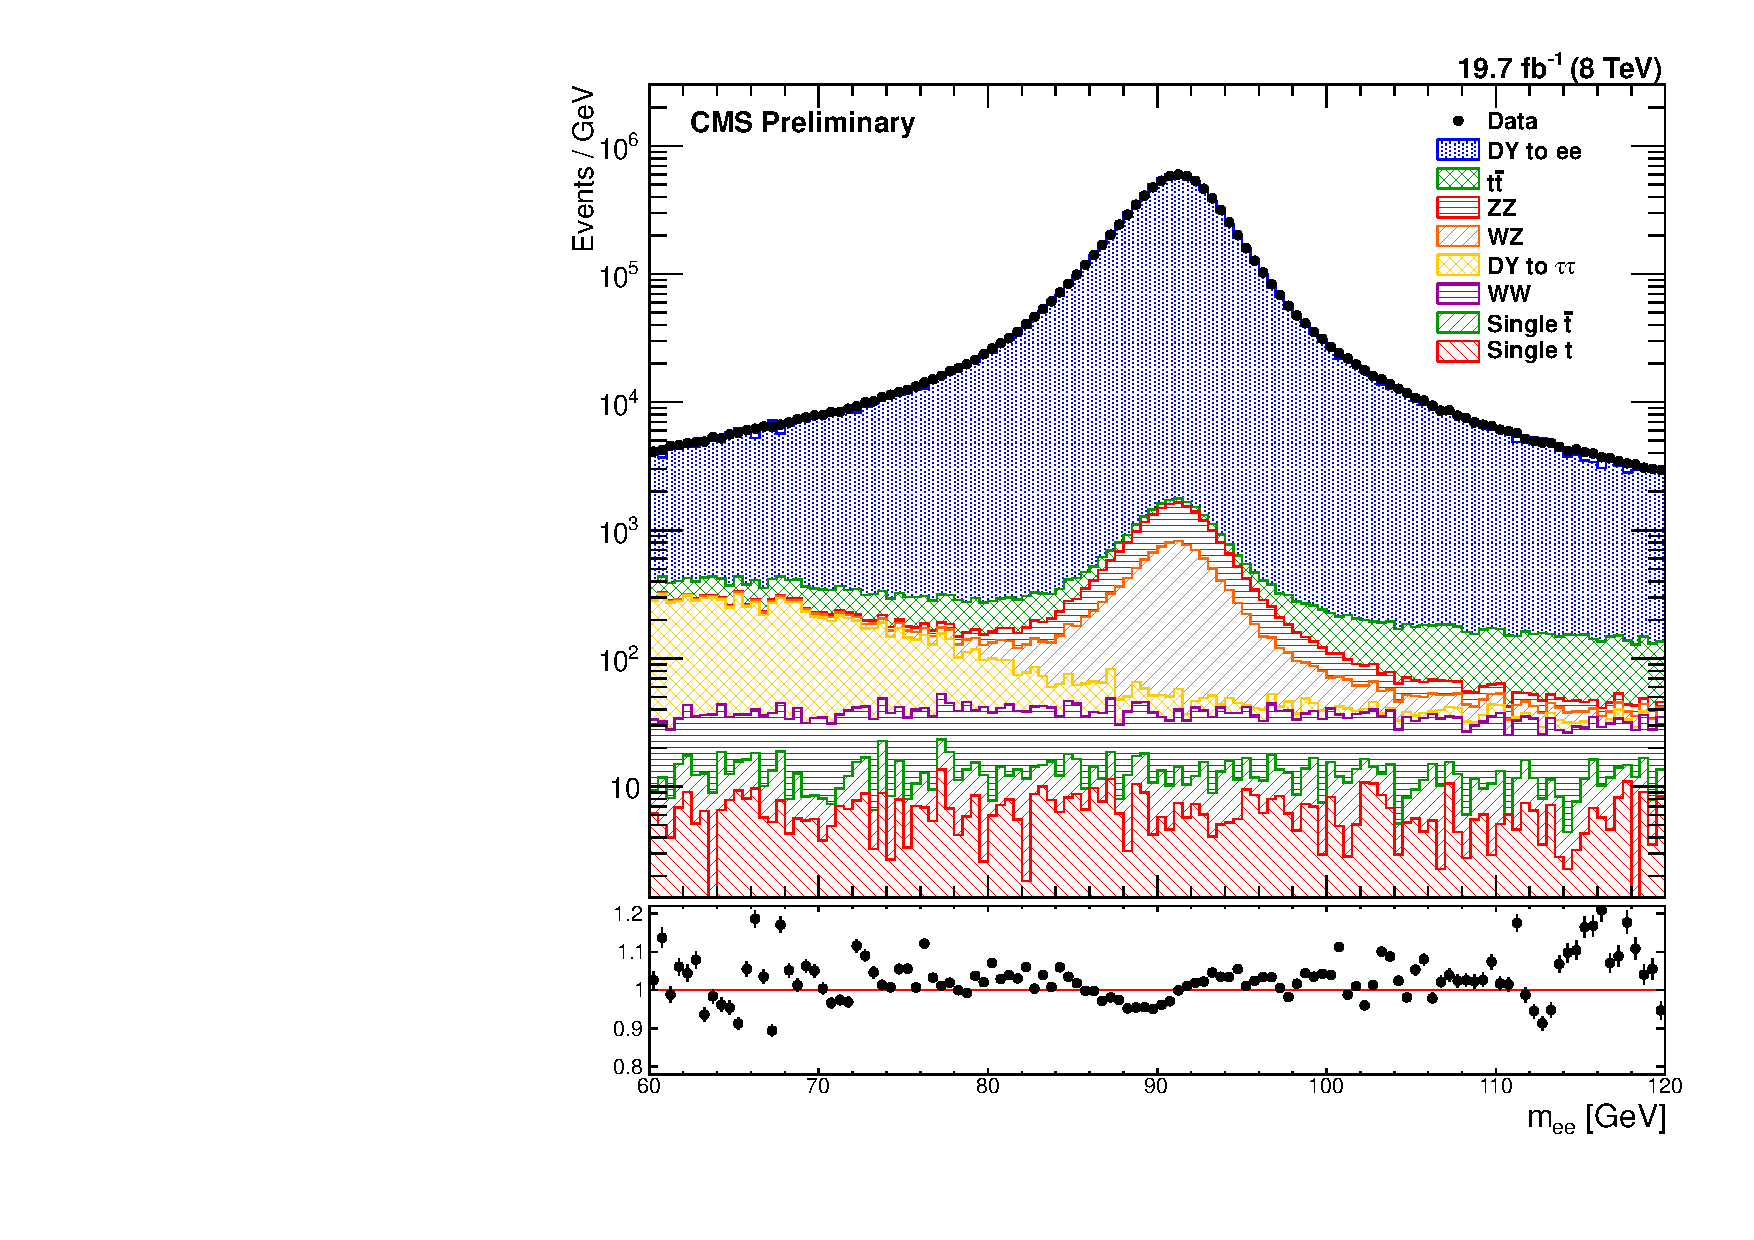
\includegraphics[width=\textwidth]{figures/z_mass_fine_powheg.pdf}
    \caption[
        The \mee distribution of events in data and MC with \POWHEG signal MC.
    ]{
        The \mee distribution of all events passing the final selection in data
        (points) and \POWHEG signal MC and the background MC samples
        (histograms).
    }
    \label{fig:z_mass_powheg}
\end{figure}

\begin{figure}[!htbp]
    \centering
    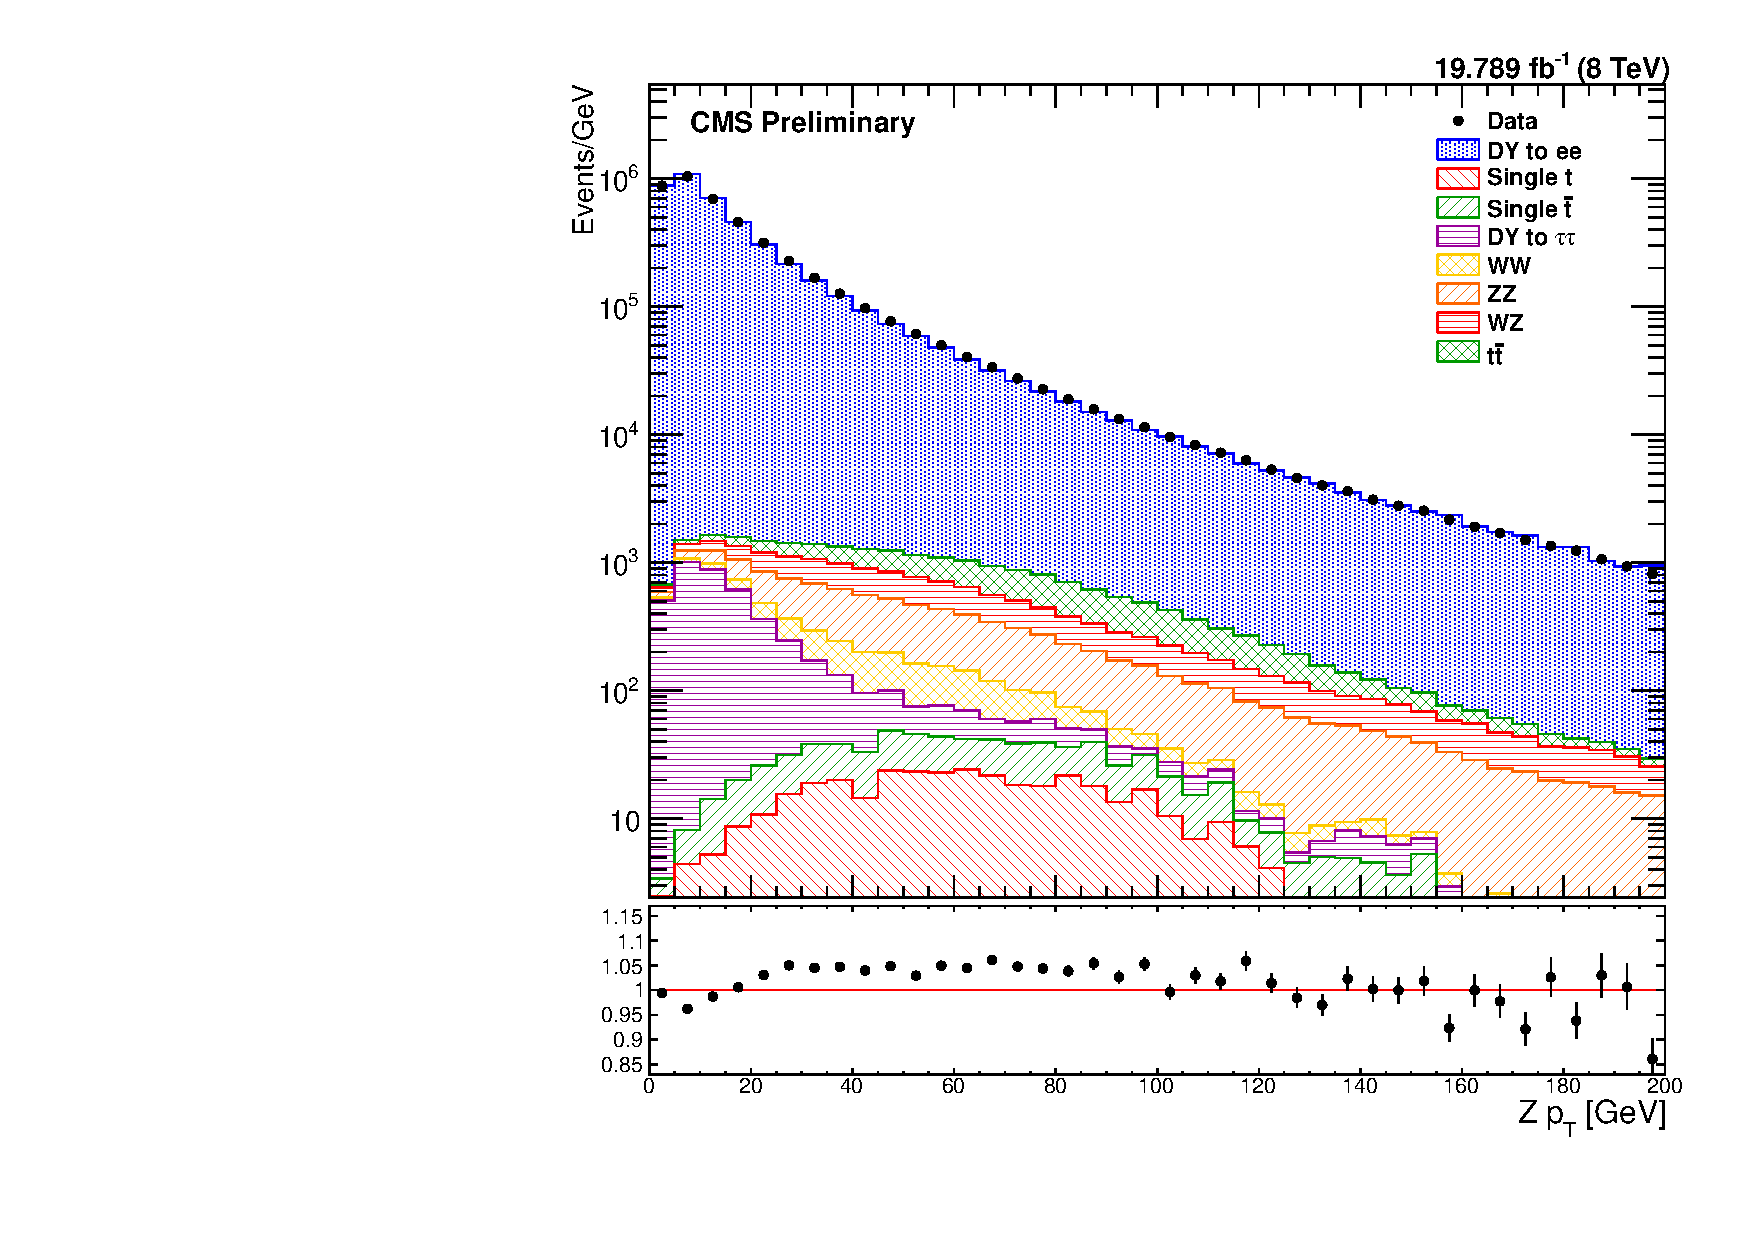
\includegraphics[width=\textwidth]{figures/z_pt.pdf}
    \caption[
        The $\pt$ distribution of \Z bosons in data and MC with \MADGRAPH
        signal MC.
    ]{
        The $\pt$ distribution of \Z bosons for all events passing the final
        selection in data (points) and \MADGRAPH signal MC and the background
        MC samples (histograms).
    }
    \label{fig:z_pt}
\end{figure}

\begin{figure}[!htbp]
    \centering
    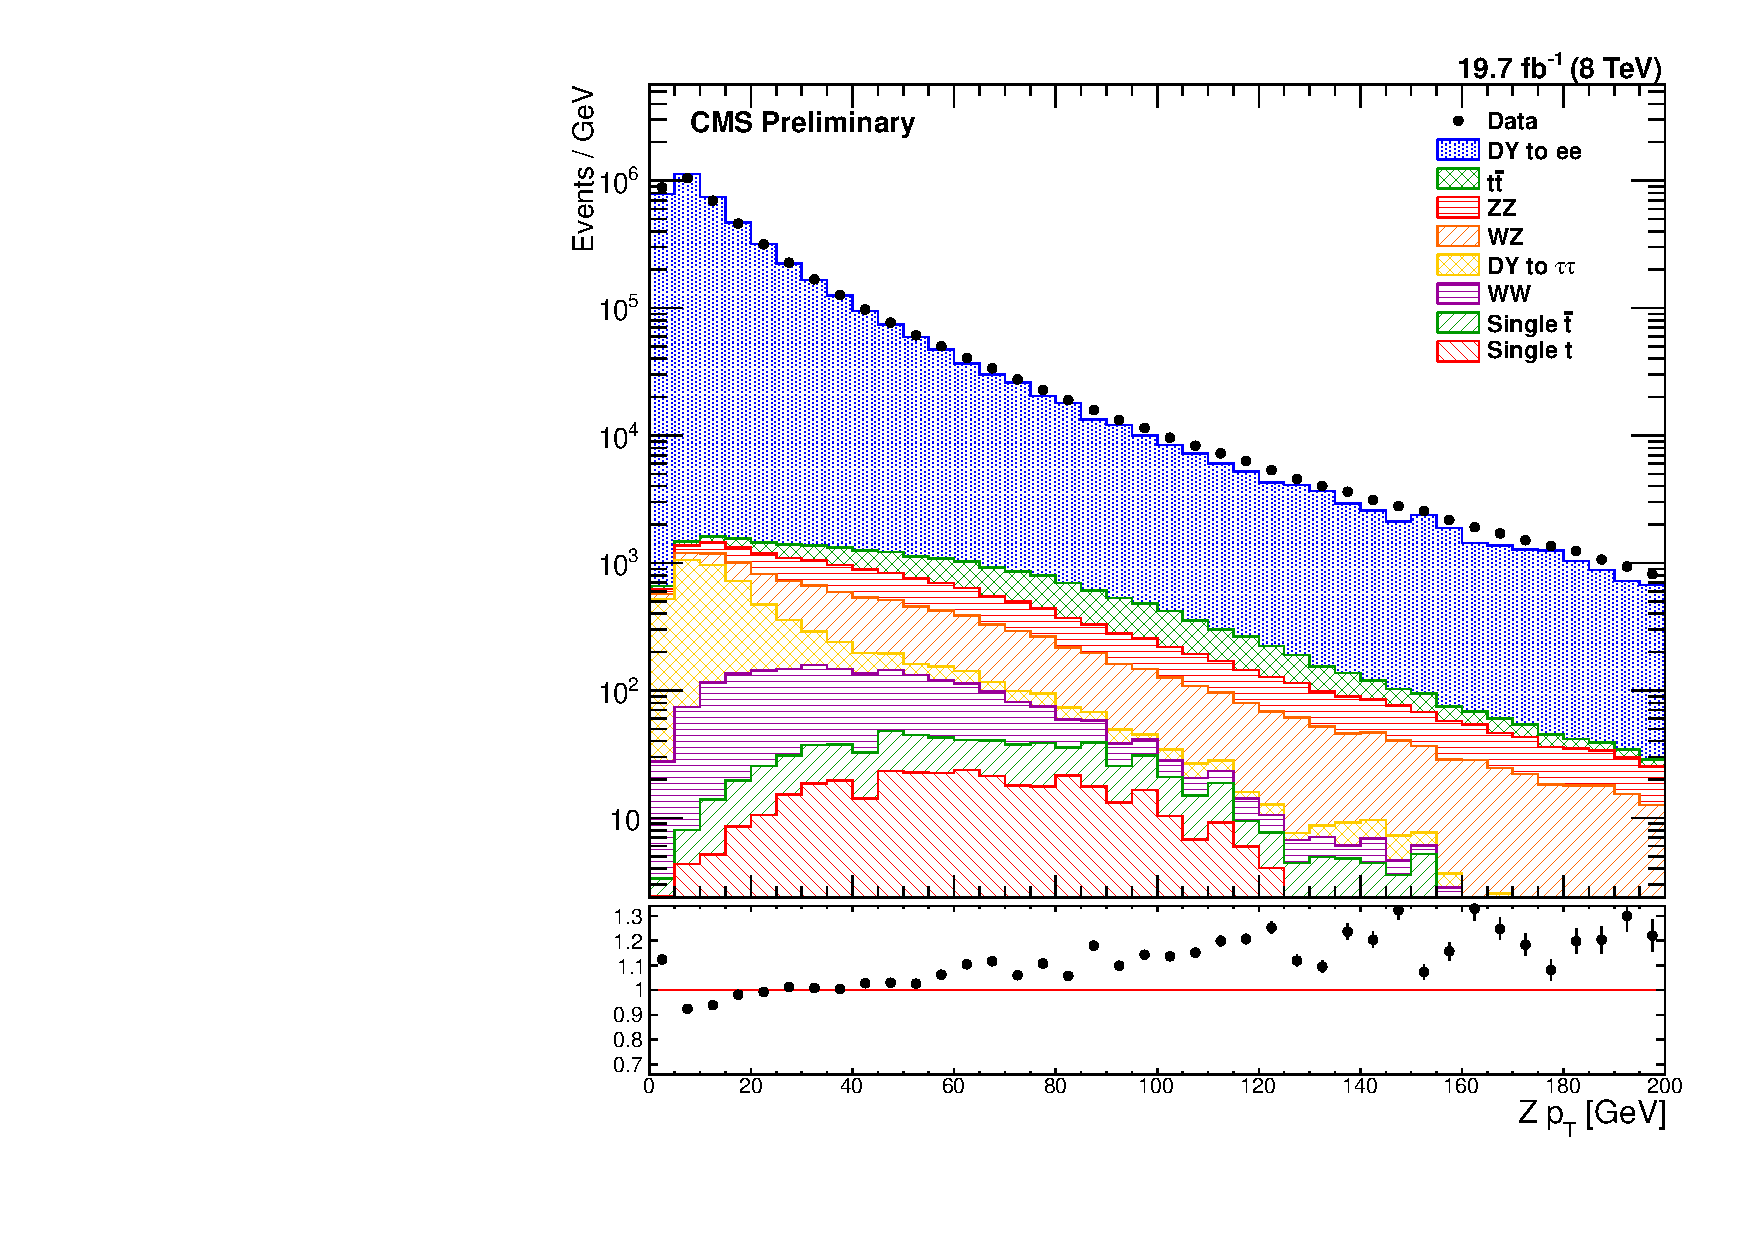
\includegraphics[width=\textwidth]{figures/z_pt_powheg.pdf}
    \caption[
        The $\pt$ distribution of \Z bosons in data and MC with \POWHEG signal
        MC.
    ]{
        The $\pt$ distribution of \Z bosons for all events passing the final
        selection in data (points) and \POWHEG signal MC and the background
        MC samples (histograms).
    }
    \label{fig:z_pt_powheg}
\end{figure}

\begin{figure}[!htbp]
    \centering
    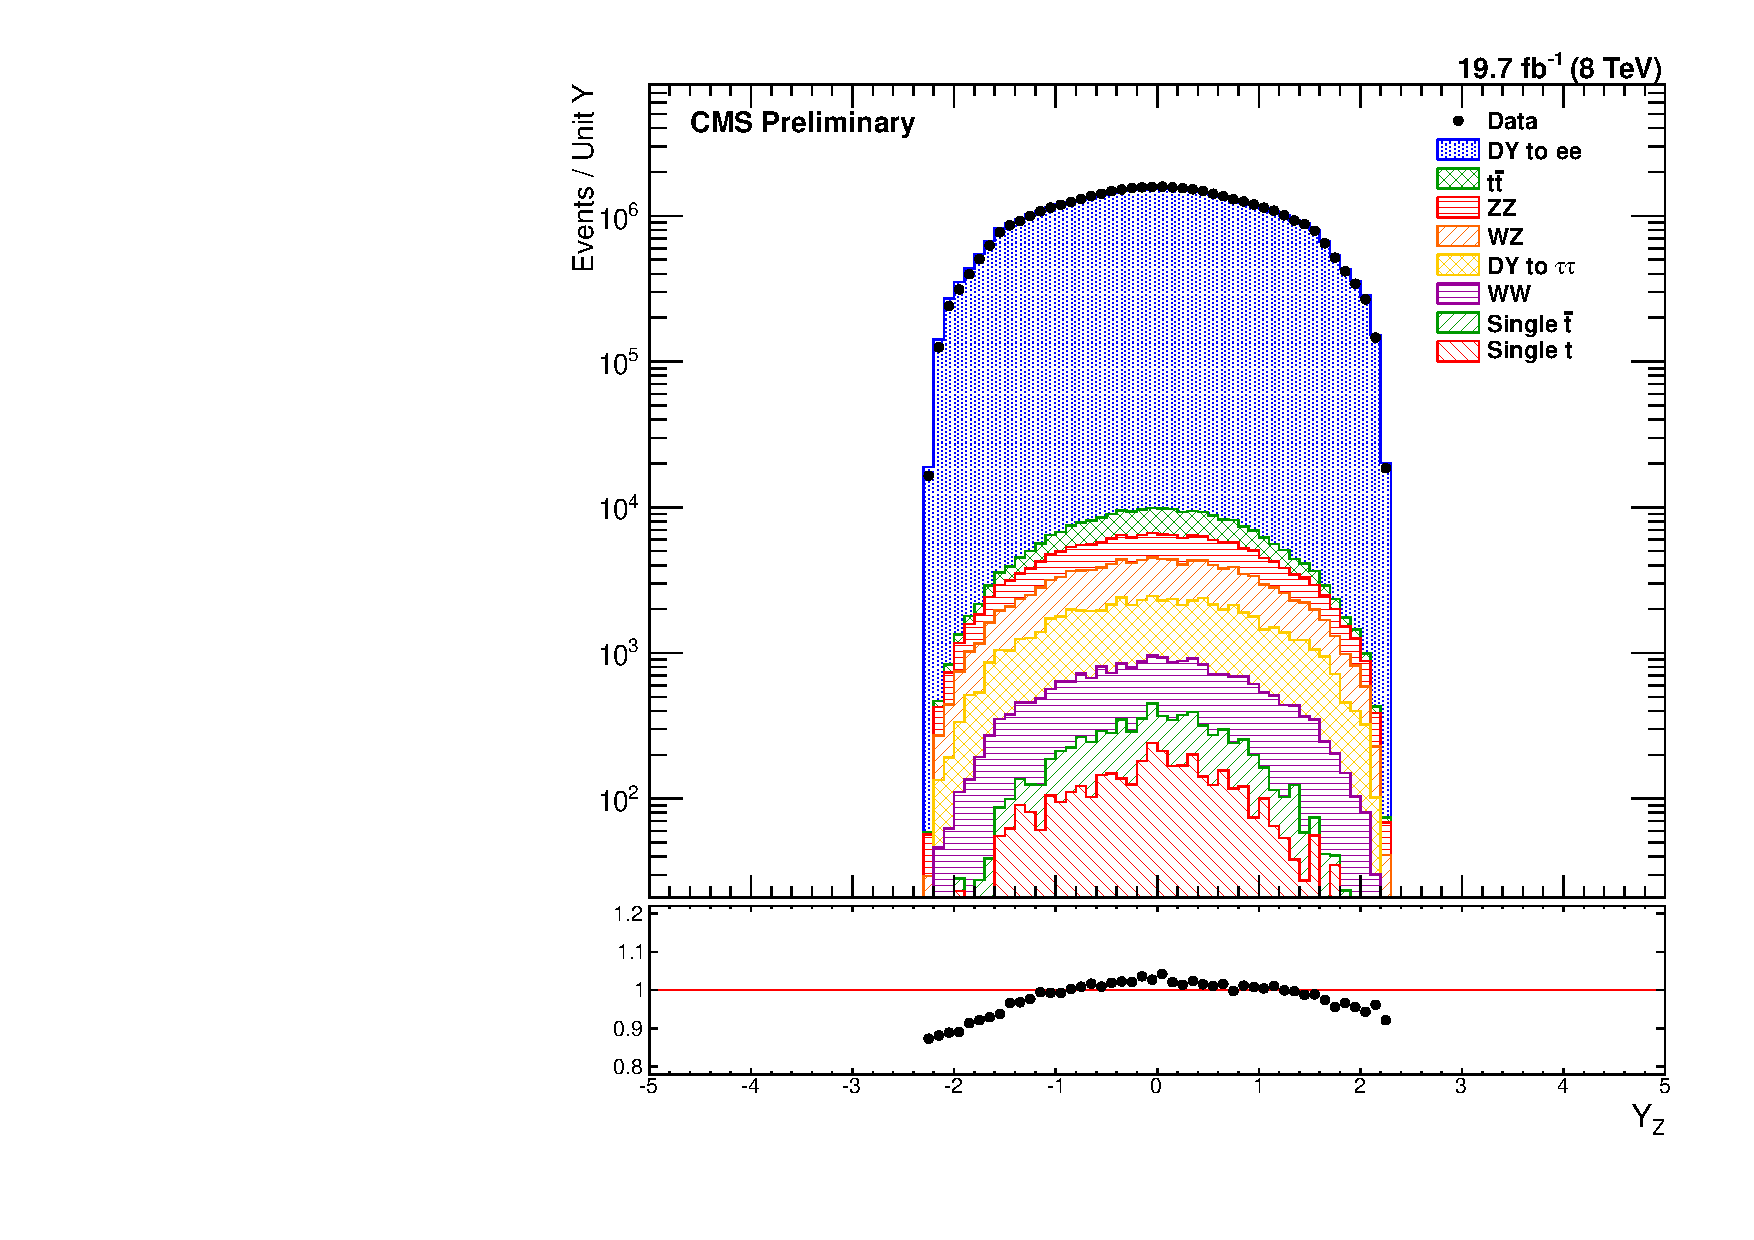
\includegraphics[width=\textwidth]{figures/z_rapidity.pdf}
    \caption[
        The $\rapidity$ distribution of \Z bosons in data and MC with \MADGRAPH
        signal MC.
    ]{
        The $\rapidity$ distribution of \Z bosons for all events passing the
        final selection in data (points) and \MADGRAPH signal MC and the
        background MC samples (histograms).
    }
    \label{fig:z_rapidity}
\end{figure}

\begin{figure}[!htbp]
    \centering
    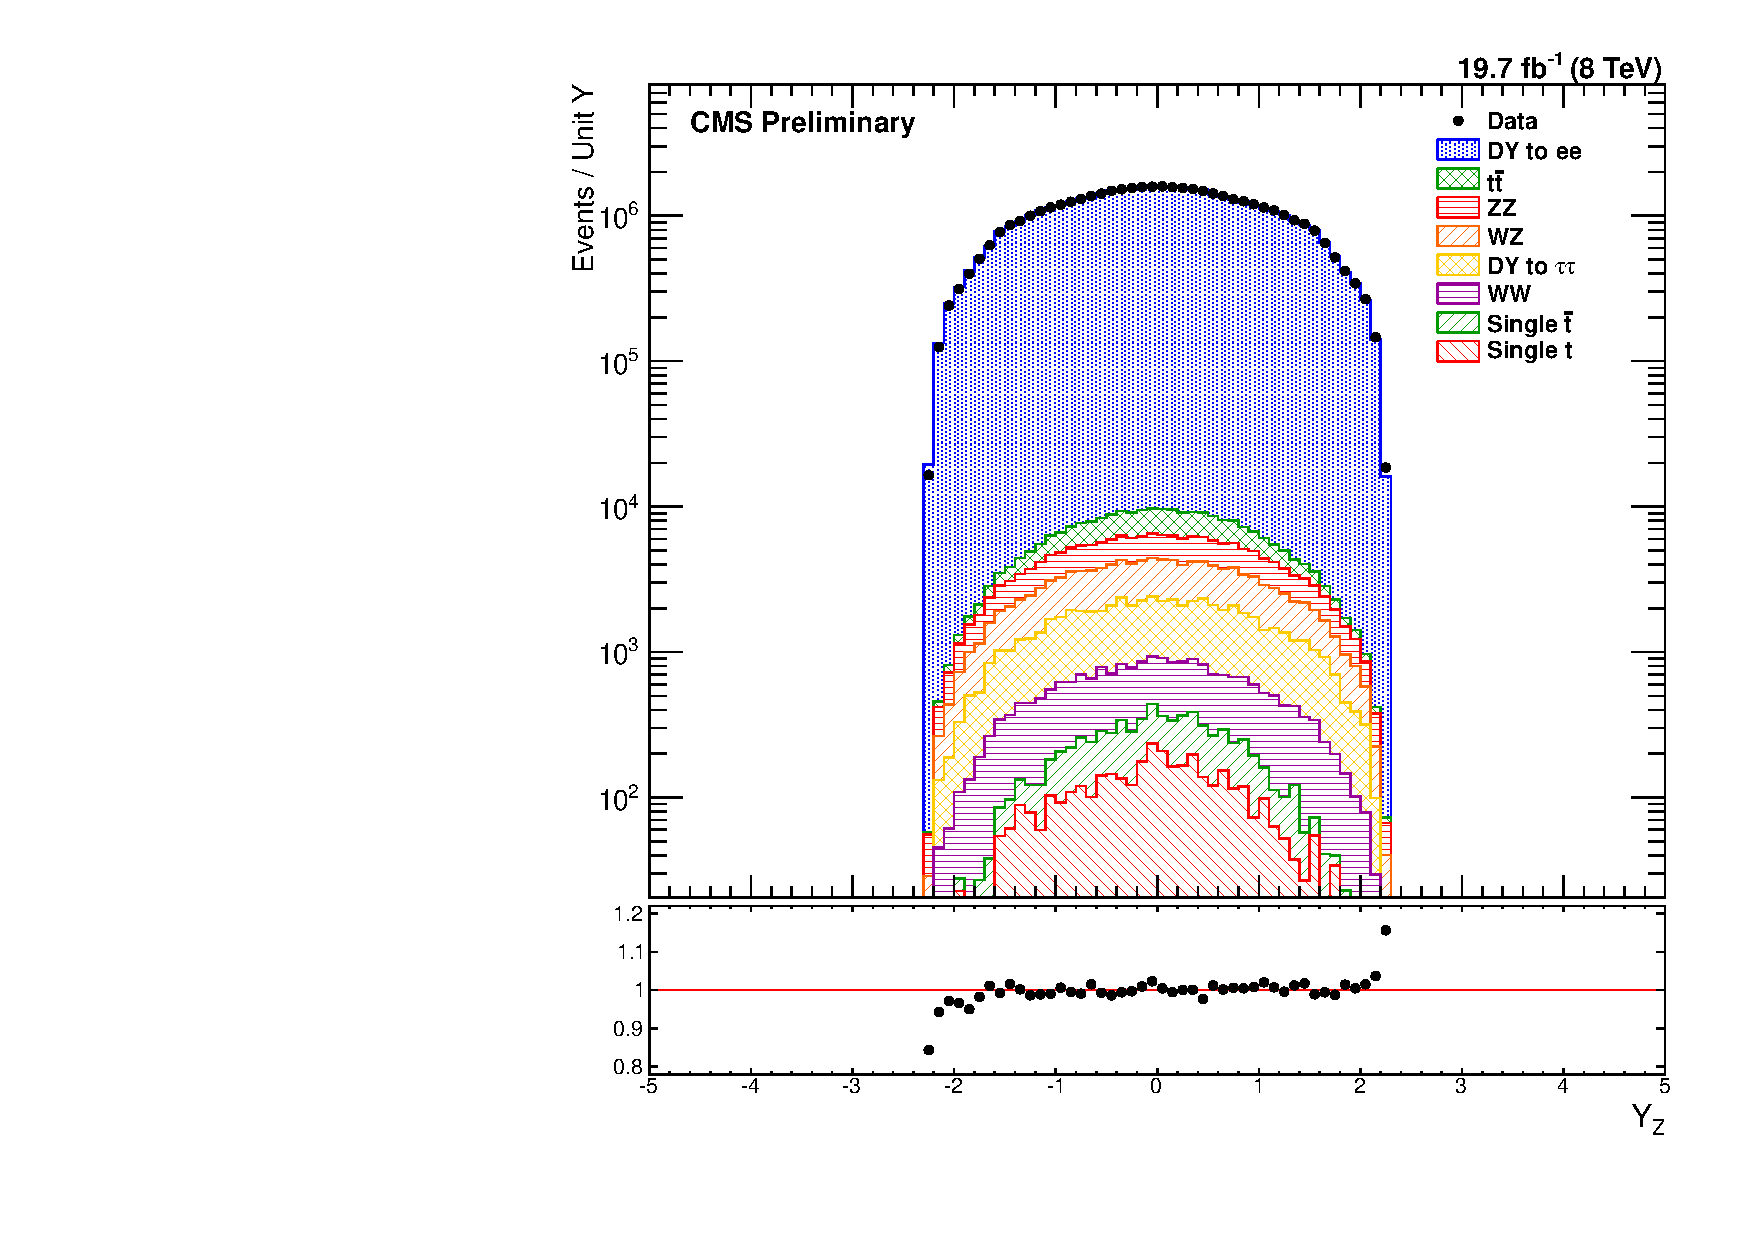
\includegraphics[width=\textwidth]{figures/z_rapidity_powheg.pdf}
    \caption[
        The $\rapidity$ distribution of \Z bosons in data and MC with \POWHEG
        signal MC.
    ]{
        The $\rapidity$ distribution of \Z bosons for all events passing the
        final selection in data (points) and \POWHEG signal MC and the
        background MC samples (histograms).
    }
    \label{fig:z_rapidity_powheg}
\end{figure}

\section{Background Estimation}
\label{sec:background}

The distribution of background events is estimated using the MC samples
discussed in \SEC~\ref{ssec:monte_carlo}, with the exception of the \QCDjets
and \wjets backgrounds, which are computed using data. The various MC samples
are reweighed so that they have equivalent luminosity to the data. The MC
datasets also have various corrections applied which are discussed in
\SEC~\ref{sec:scale_factors}. These scale factors are applied as weights to
each MC event in order to make them better match the data.

After the reweighting, the selection requirements are applied to to the MC. The
number of events that survive the selection are taken as the number in our
data, and are subtracted off from the data events.

Overall, the selection requirements discussed in the previous sections leave a
very pure sample of \Z boson events. 99.44\% of events are signal. The dominant
backgrounds are the diboson backgrounds and \ttbar. We define \Z bosons
produced in association another weak boson as a background because of their
different production mechanism as opposed to single \Z boson events. The
fraction of events from each of the considered backgrounds is listed in
\TAB~\ref{table:bg_percentages}.

\begin{table}[h]
\centering
\spacerows{1.2}
\begin{center}
    \begin{tabular}{@{}l r r@{}}
    \toprule
    Process                        & of total & of background \\
    \midrule
    Signal: $\DYtoee$              & 99.44\%  & N.A. \\
    \ttbar                         & 0.15\%   & 26.6\% \\
    $\Z\Z$                         & 0.12\%   & 21.6\% \\
    $\W\Z$                         & 0.12\%   & 21.4\% \\
    $\DYtotautau$                  & 0.09\%   & 16.2\% \\
    $\W\W$                         & 0.03\%   & 5.6\% \\
    $\QCDjets \text{ and } \wjets$ & 0.03\%   & 5.6\% \\
    $t\W \text{ and } \tbar\W$     & 0.02\%   & 2.9\% \\
    \bottomrule
    \end{tabular}
\end{center}
\caption[
    The compisition of the data sample.
]{
    Data sample composition as a percentage of the total, as well as the
    backgrounds as a percentage of all background events.
}
\label{table:bg_percentages}
\end{table}

%\begin{figure}[!htbp]
%    \centering
%    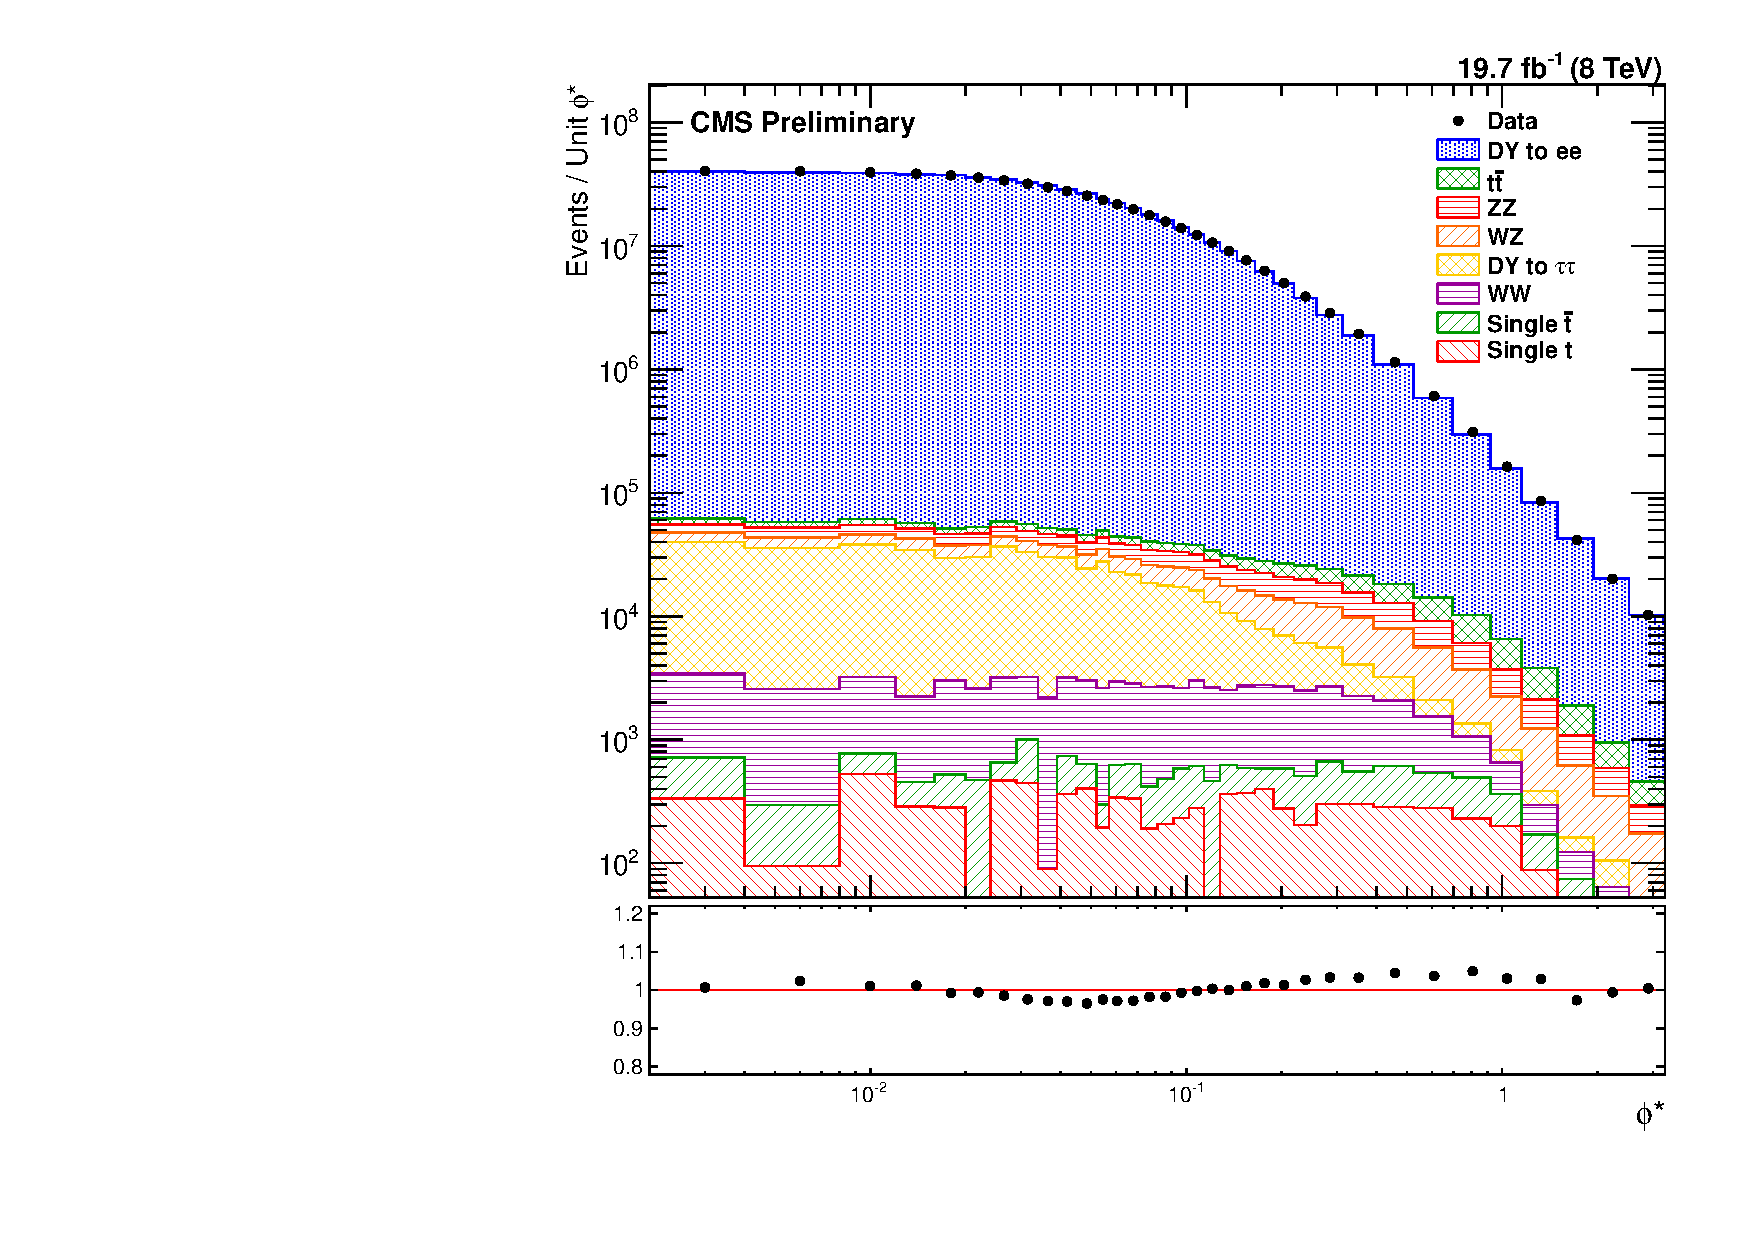
\includegraphics[width=\textwidth]{figures/phistar.pdf}
%    \caption[
%        The \phistar distribution of events in data and MC.
%    ]{
%        The \phistar distribution of events in data (points) and MC
%        (histograms) for events passing the full analysis selection.
%    }
%    \label{fig:phistar_background}
%\end{figure}

\subsection{\texorpdfstring{\emu}{Electron--Muon} Control Sample}
\label{ssec:emu_sample}

Many of the backgrounds---specifically $\ttbar$, $\W\W$, $\DYtotautau$, and
$\ttbar$---produce leptons via independent decay chains. Therefore, the flavor
of the two leptons is not constrained to be the same. An electron--muon
(\emu) background dominated control sample is used to test how well the MC
reproduce the various backgrounds.

Events for the \emu sample are selected from data taken with the
\SingleMuonTrigger. This trigger required a single muon with $\pt > 24 \GeV$
and $|\eta| < 2.1$. Events selected from the dataset provided by this trigger
are required to have one muon with $\pt > 25 \GeV$ and $|\eta| < 2.1$ and one
electron with $\pt > 20 \GeV$ and $|\eta| < 2.4$. In order to further suppress
\Z decays, events are rejected if there is a third lepton of either flavor with
$\pt > 20 \GeV$ and $|\eta| < 2.4$. \FIG~\ref{fig:emu_background_check} shows a
comparison of the MC and data in the control region. Although no deviations
from \num{1} are seen, this ratio is taken as a scale factor to correct the
previously listed backgrounds in each bin. A compairison of the \Ztomumu MC
samples before and after this scale factor is applied is shown in
\FIG~\ref{fig:emu_after_correction}.

\begin{figure}[!htbp]
    \centering
    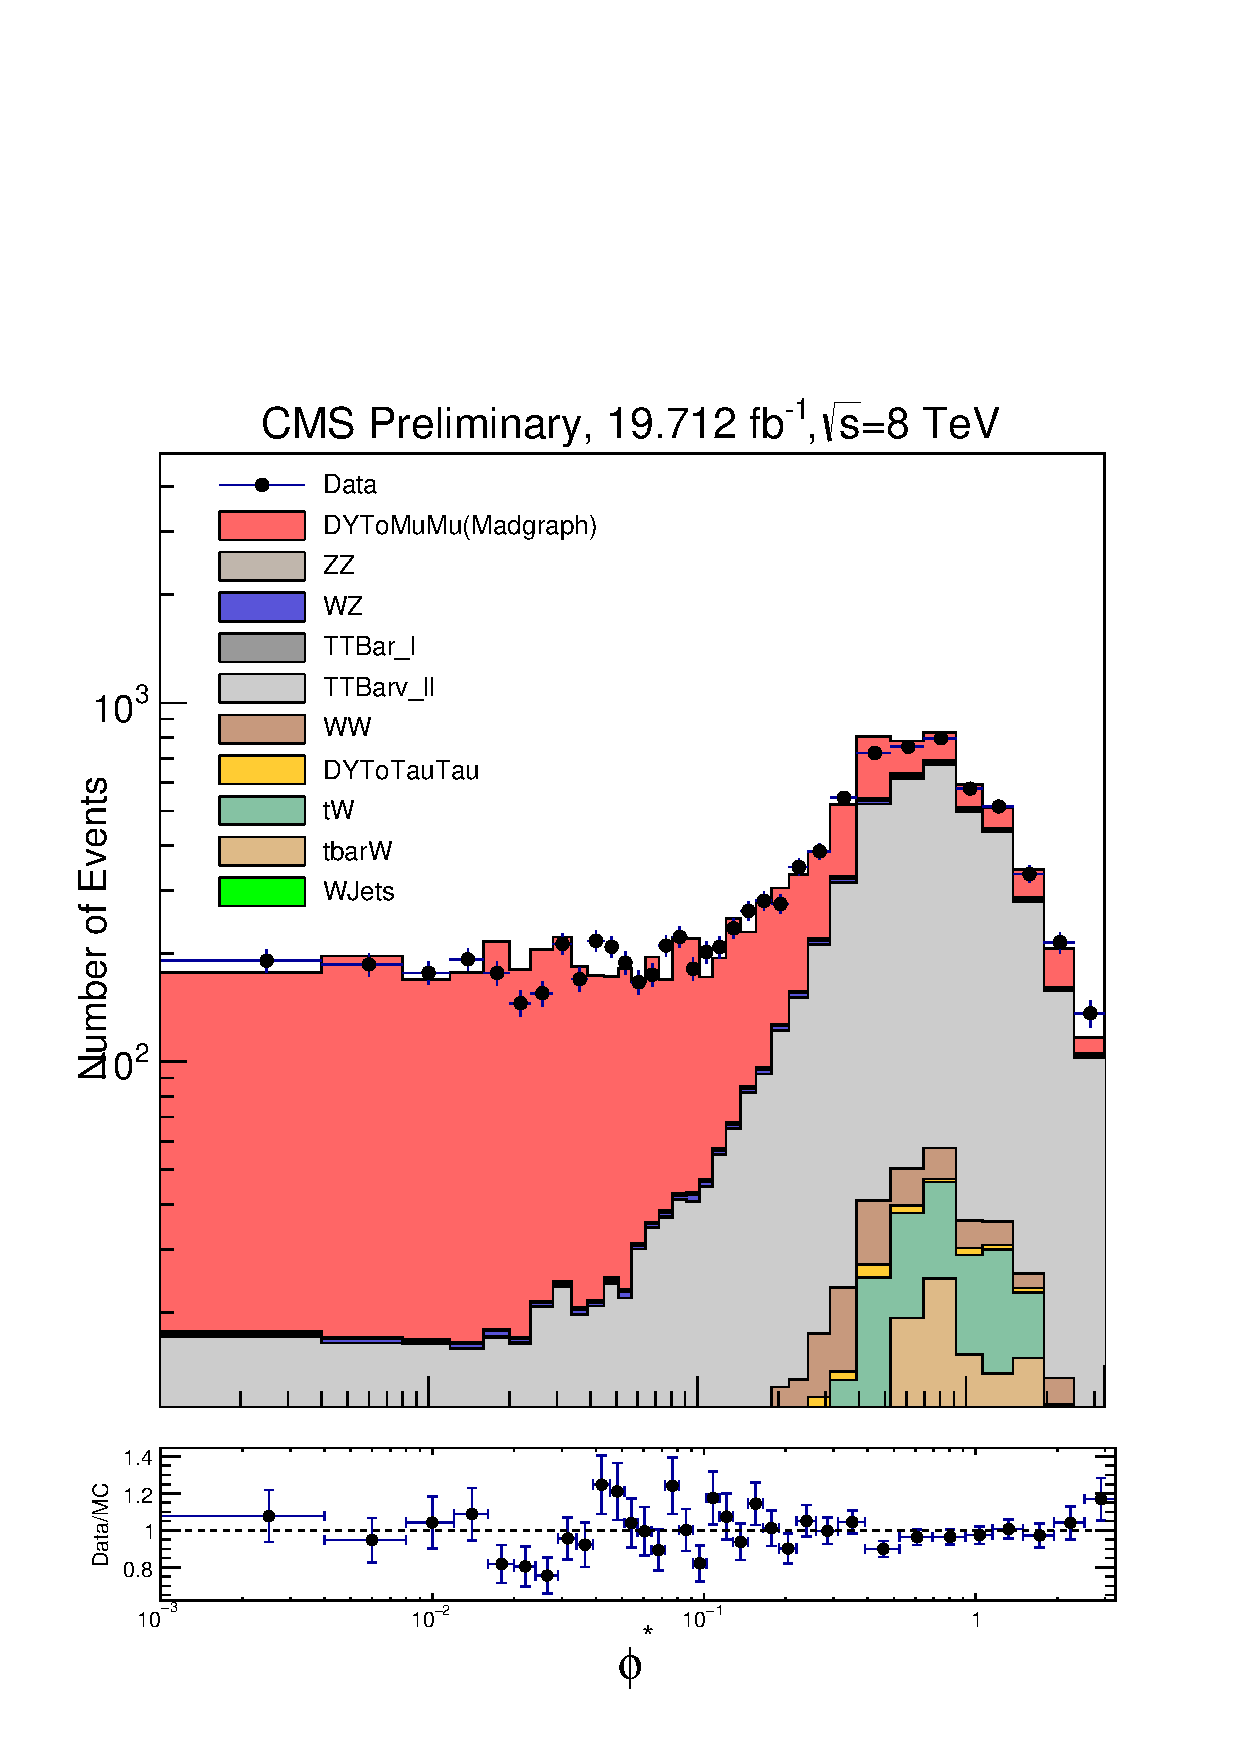
\includegraphics[width=\textwidth]{figures/phistar_emu.pdf}
    \caption[
        The \phistar distribution of events from the \emu control sample.
    ]{
        The \phistar distribution of events from the \emu control sample. The
        data (points) match the MC (histograms) expectation well. The ratio,
        shown in the bottom plot, is taken as a scale factors and used to
        correct the backgrounds in each bin.
    }
    \label{fig:emu_background_check}
\end{figure}

\begin{figure}[!htbp]
    \centering
    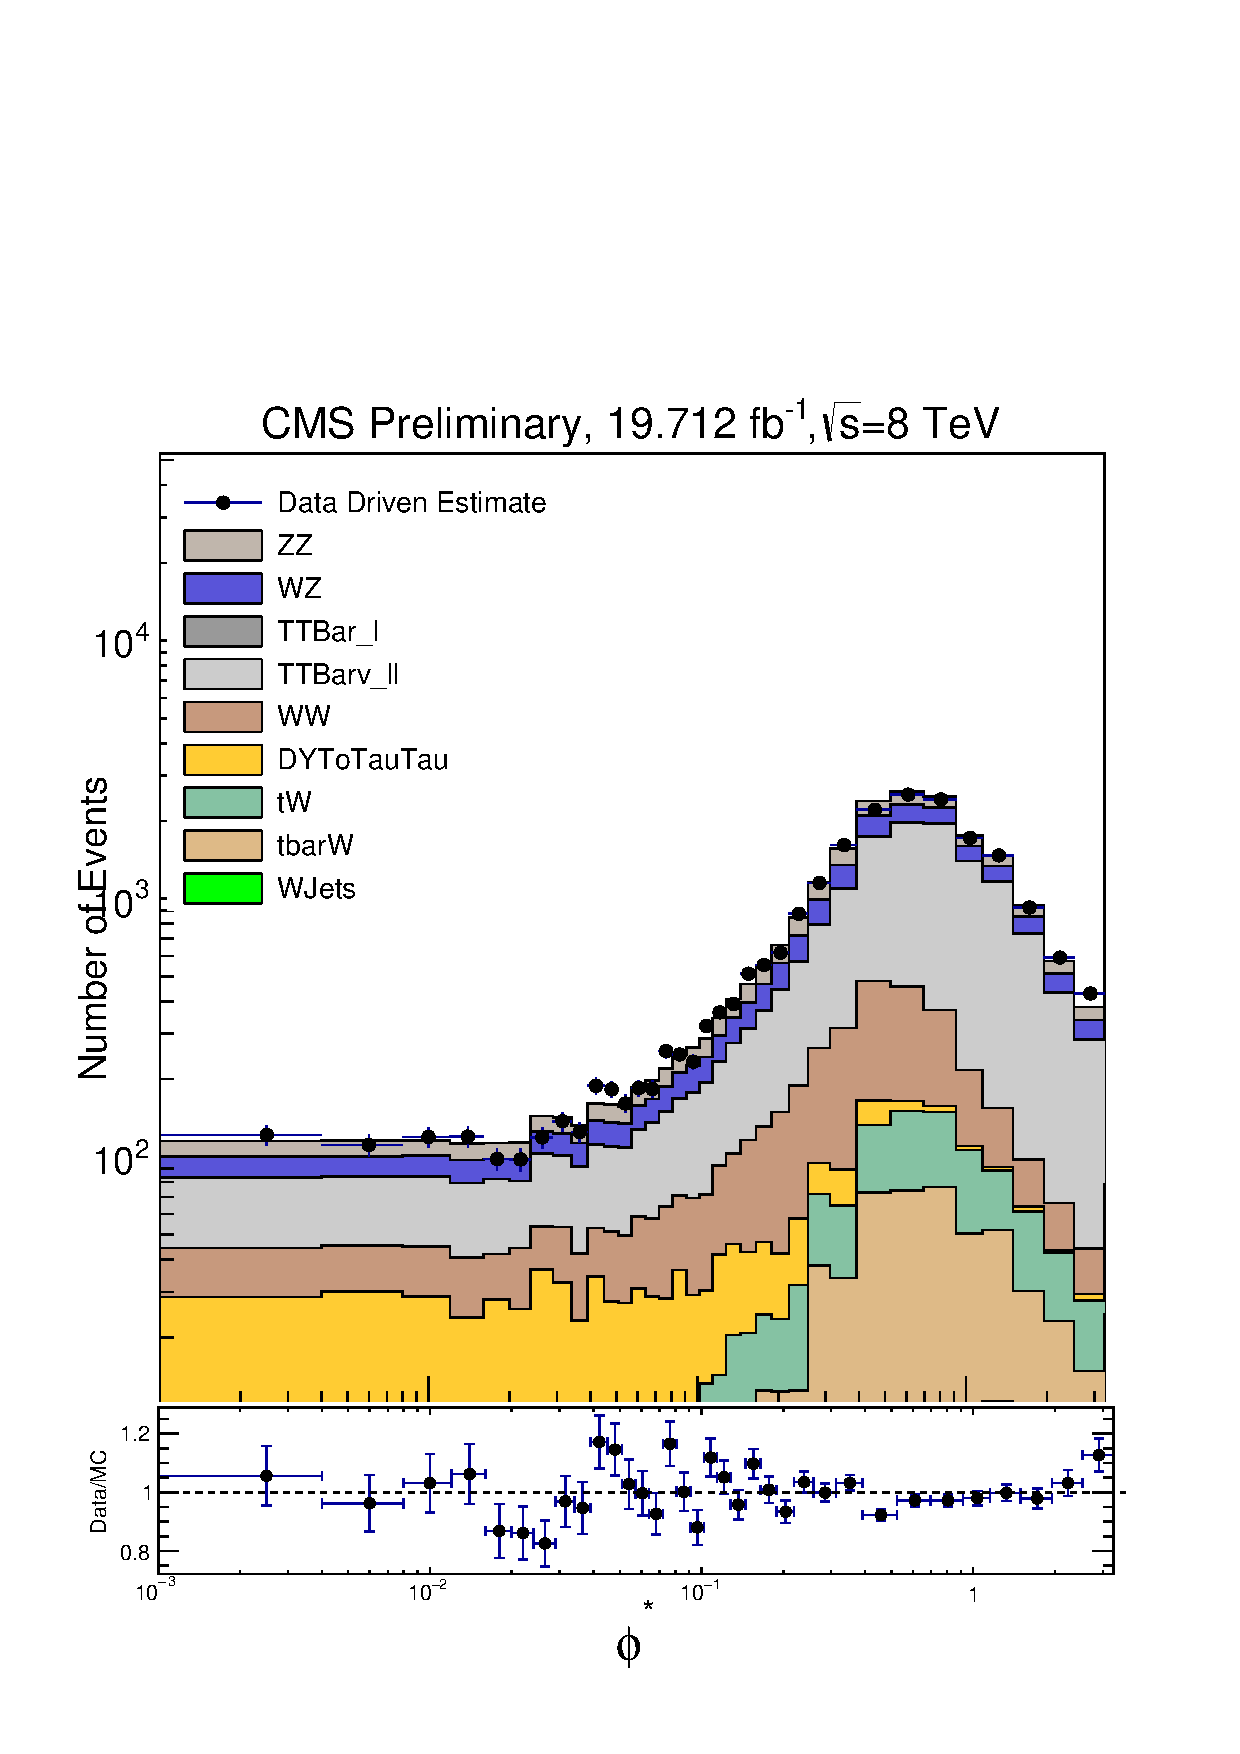
\includegraphics[width=\textwidth]{figures/emu_check.pdf}
    \caption[
        The \phistar distribution of \Ztomumu events in MC before and after the
        \emu correction.
    ]{
        The \phistar distribution of \Ztomumu events in MC before and after the
        \emu correction. The samples without the \emu derived scale factors
        applied are shown in the histograms, while the points show the sum of
        all the MC samples after the scale factors are applied.
    }
    \label{fig:emu_after_correction}
\end{figure}

This method could not be used to calibrate the $\Z\Z$ and $\Z\W$ background MC
samples as they contain actual \Z bosons. Instead a 20\% uncertainty is taken
on their theoretical cross-section.

\subsection{QCD Background Estimation}
\label{ssec:qcd_background}

The centrally produced \QCDjets and \wjets MC samples do not have enough events
to make accurate estimations of their respective background in this analysis so
instead a data driven method is employed. The same requirements as discussed in
\SEC~\ref{ssec:electron_selection} are applied to both the data and the MC
samples with the additional requirement that both electrons must have the same
charge. This additional selection requirement removes most of the signal while
removing only half of the expected \QCDjets and \wjets backgrounds because
these processes are independent and hence there is no correlation between the
charge of the two leptons.

The data and MC are divided into subsamples with each subsample corresponding
to a bin in the \phistar distribution. The \mee distribution of the events in
each data subsample is fit with a combination of an MC template and an analytic
background function.

The MC templates used in the fit are created by reweighting each MC sample to
have the same luminosity as the data. All of these MC samples---both the
\MADGRAPH signal sample and the various background samples---in each \phistar
bin are added together, and their shape is used as the template in the fit with
its amplitude as a free parameter.

The analytic background function, $\BGFunc$, is the same function used by
Haupt to model the \QCDjets and \wjets backgrounds in his \Ztoee shape
measurement \cite{haupt_2011}. It is composed of a falling exponential---which
fits the general shape of the \QCDjets and \wjets background
distribution---multiplied by a complementary error function---which cuts off
the exponential at low mass. The exact form of this function is given by
\EQ~\ref{eq:haupt_function}. The sum of the template and the background
function is given by \EQ~\ref{eq:qcd_fit_function}.

\begin{equation}\label{eq:haupt_function}
    \BGFuncArgs = e^{- \gamma x} \erfc \left( \frac{\varepsilon - x}{\delta} \right)
\end{equation}

\begin{equation}\label{eq:qcd_fit_function}
    \alpha \, \MCTemplate + \beta \, \BGFuncArgs
\end{equation}

The background due to \QCDjets and \wjets in each \phistar bin is taken to be
the integral of the analytic background component from \MassRange multiplied by
two. The factor of two comes from the fact that the estimate was performed
using only events containing same-charge electrons while the full analysis
accepts both same- and opposite-charge events which are equally likely in the
background. The estimated \QCDjets and \wjets backgrounds in each \phistar bin
are showing in \FIG~\ref{fig:qcd_phistar}. Two example fits are shown in
\FIG~\ref{fig:qcd_example_fits}. All of the fits are shown in
\APP~\ref{app:qcd_fits}.

\begin{figure}[!htbp]
    \centering
    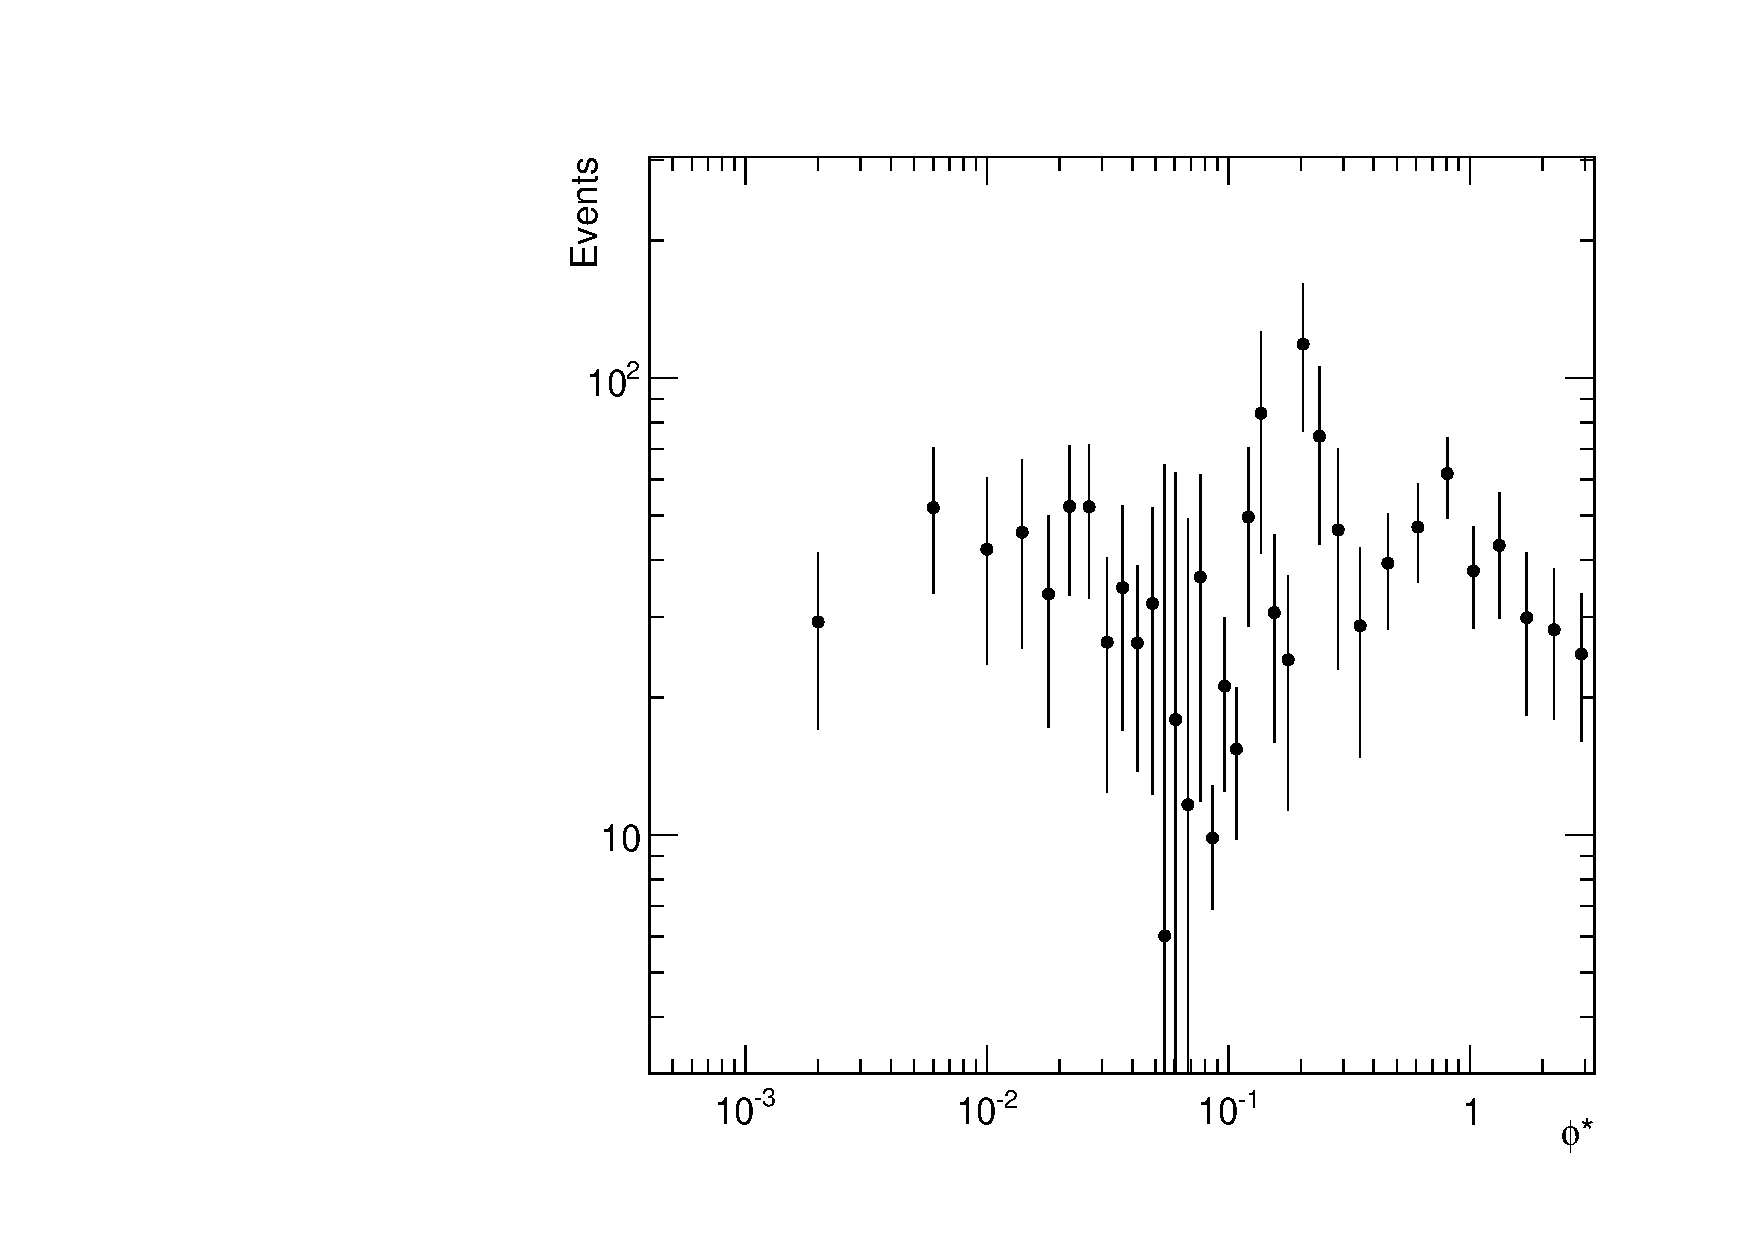
\includegraphics[width=\textwidth]{figures/qcd_phistar.pdf}
    \caption[
        The integral of the analytic background function in each \phistar bin.
    ]{
        The integral of the analytic background function, \BGFunc, in each
        \phistar bin. The number has been multiplied by two to account for the
        fact that we accept both same- and opposite-charge events.
    }
    \label{fig:qcd_phistar}
\end{figure}

\begin{figure}[!htbp]
    \centering
    \begin{subfigure}[b]{\SideBySidePlotWidth}
        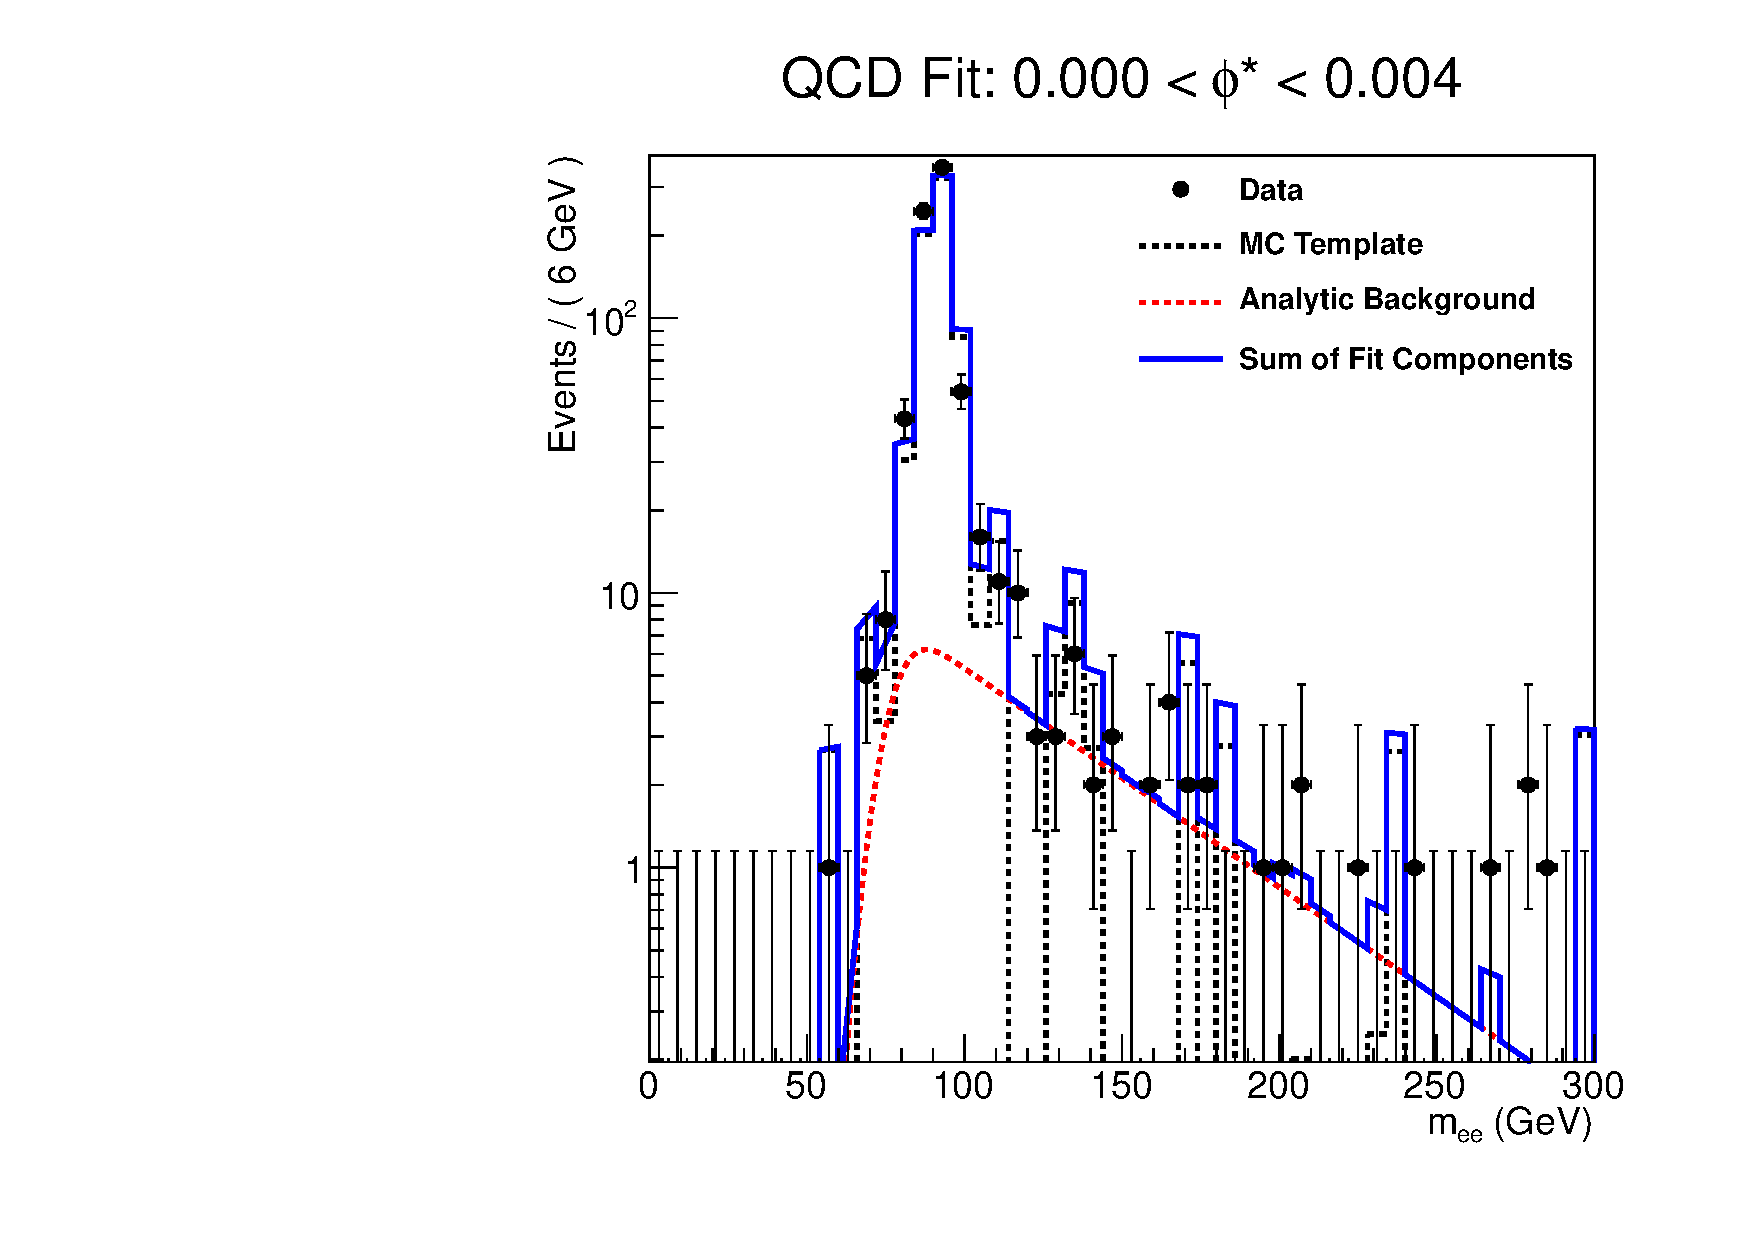
\includegraphics[width=\linewidth]{figures/qcd_fits/qcd_fit_plot_for_01.pdf}
        \caption{}
        \label{fig:qcd_fit_example_01}
    \end{subfigure}%
    % The comment right after suppresses white space that would push the images
    % to new lines
    \begin{subfigure}[b]{\SideBySidePlotWidth}
        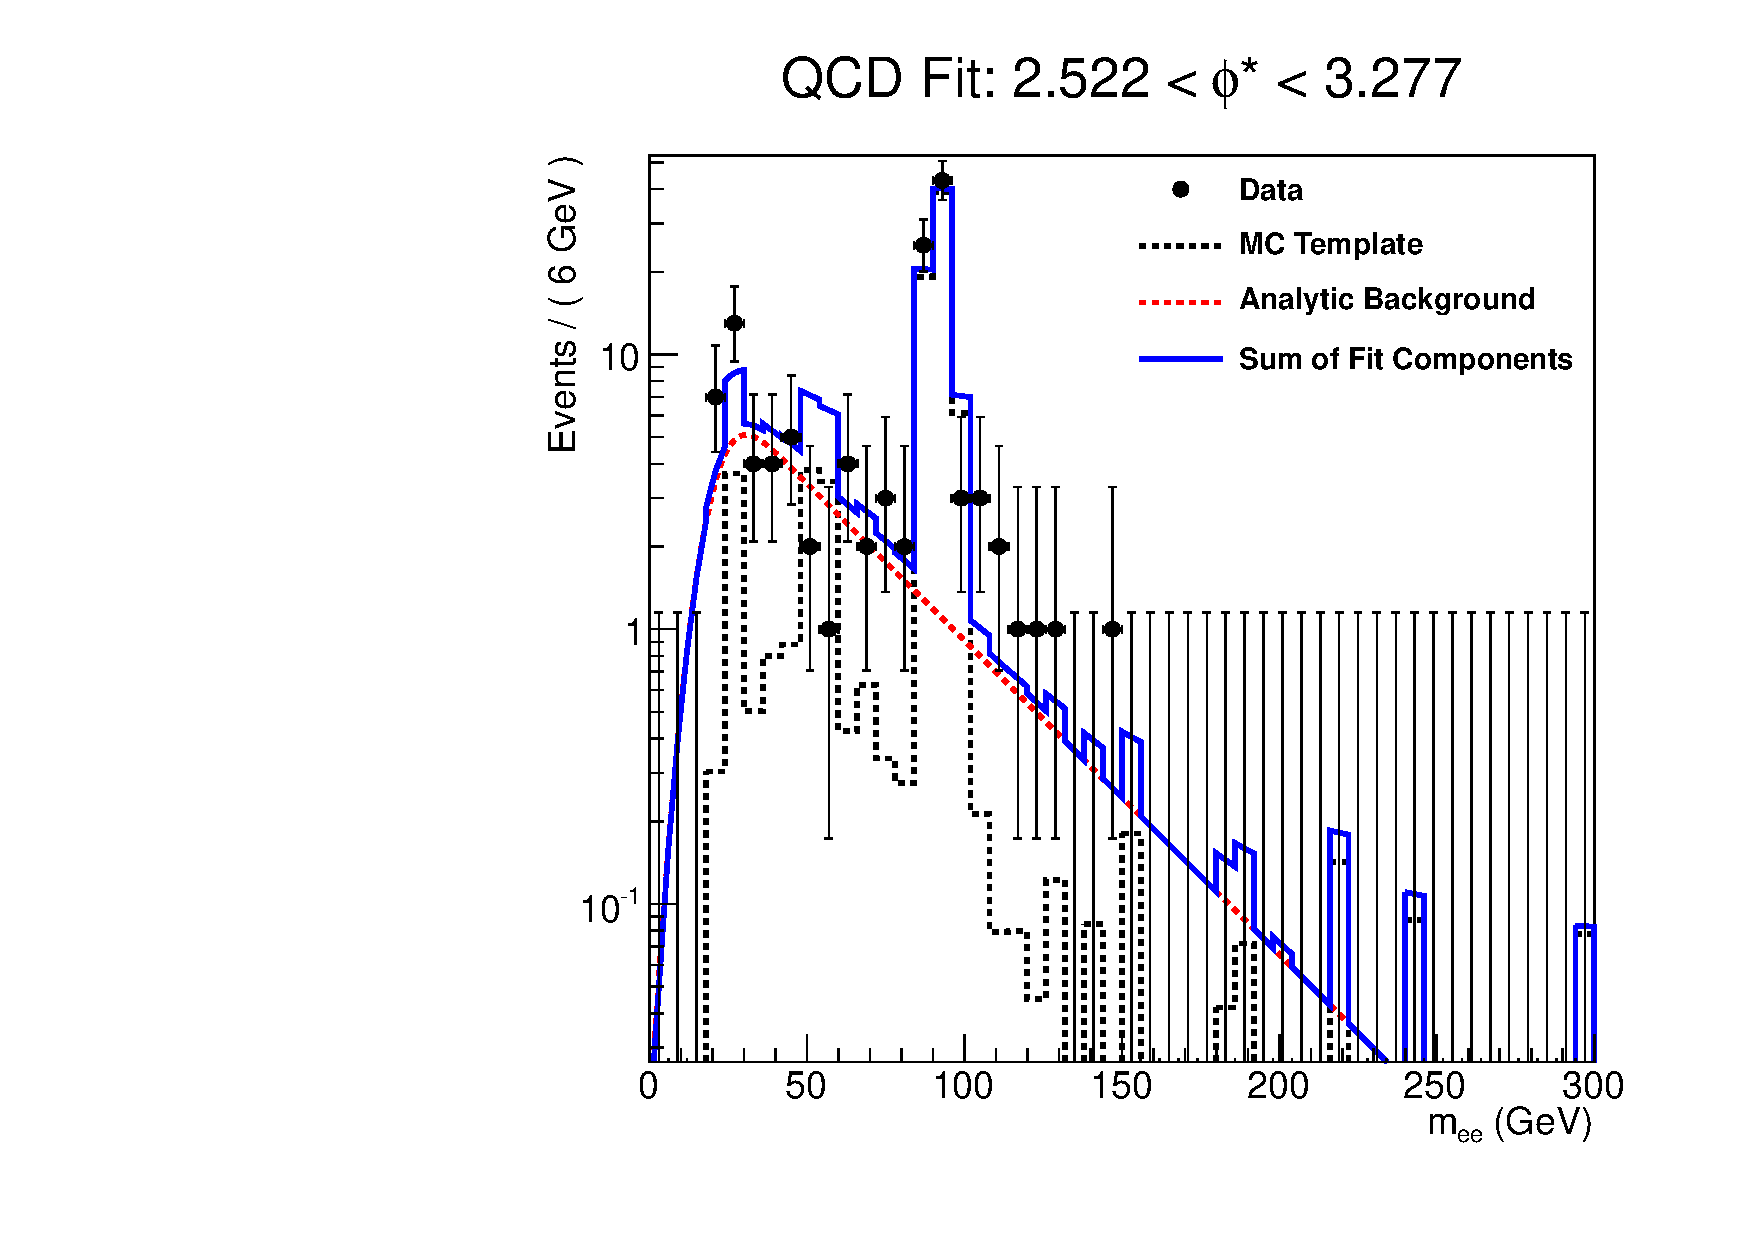
\includegraphics[width=\linewidth]{figures/qcd_fits/qcd_fit_plot_for_34.pdf}
        \caption{}
        \label{fig:qcd_fit_example_34}
    \end{subfigure}
    \caption[
       Examples of the \QCDjets and \wjets data-driven background fits.
    ]{
       Examples of the \QCDjets and \wjets data-driven background fits for the
       first and last \phistar bins. The data are shown as points with error
       bars, MC template as a dashed histogram, the analytic background
       function as the dashed line, and the sum of the template and function as
       a solid histogram. The full set of plots are shown in
       \APP~\ref{app:qcd_fits}.
    }
    \label{fig:qcd_example_fits}
\end{figure}

\section{Unfolding}
\label{sec:unfolding}

Particle detectors are incredibly sophisticated machines designed to make
precise measurements of the various decay products created during the
collisions. However, there are physical limitations that prevent a perfect
measurement from being made. The finite energy, momentum, and position
resolution of the various subdetectors impose limitations on the final
measurements. In order to allow our measurement to be compared to theoretical
predictions, we correct for these detector effects with a process known as
unfolding.

We unfold in two steps: first the data are unfolded to correct for bin
migration, second we correct for the imperfect efficiency of the trigger and
reconstruction. The data are unfolded against the three definitions of
generator level electrons: born, dressed, and bare as described in
\SEC~\ref{sec:electron_dressing}. Results in this chapter are shown with
dressed electrons, born and bare electrons are given in \APP\TODO{Born, Bare
Appendix}.

\subsection{Bin Migration}
\label{ssec:bin_migration}

The finite resolution of CMS's angular position measurements leads to a finite
resolution of the reconstructed \phistar distribution. Events which at the
generator level would have ended up in a certain \phistar bin may instead
migrate to one of the neighboring bins. The \phistar reconstruction resolution,
defined as $\left( \phistarGen - \phistarReco \right) / \phistarGen$, is shown
in \FIG~\ref{fig:phistar_resolution}.

MC events are used to create a response matrix that describes how generator
level events are reconstructed in CMS. This matrix is shown in
\FIG~\ref{fig:bin_migration_matrix}. The amount of bin migration, as measured
by the off-diagonal elements, is 5.5\%. Through unfolding this matrix is
inverted, allowing us to transform the data to remove the undesired bin
migration.

\begin{figure}[!htbp]
    \centering
    \begin{subfigure}[b]{\SideBySidePlotWidth}
        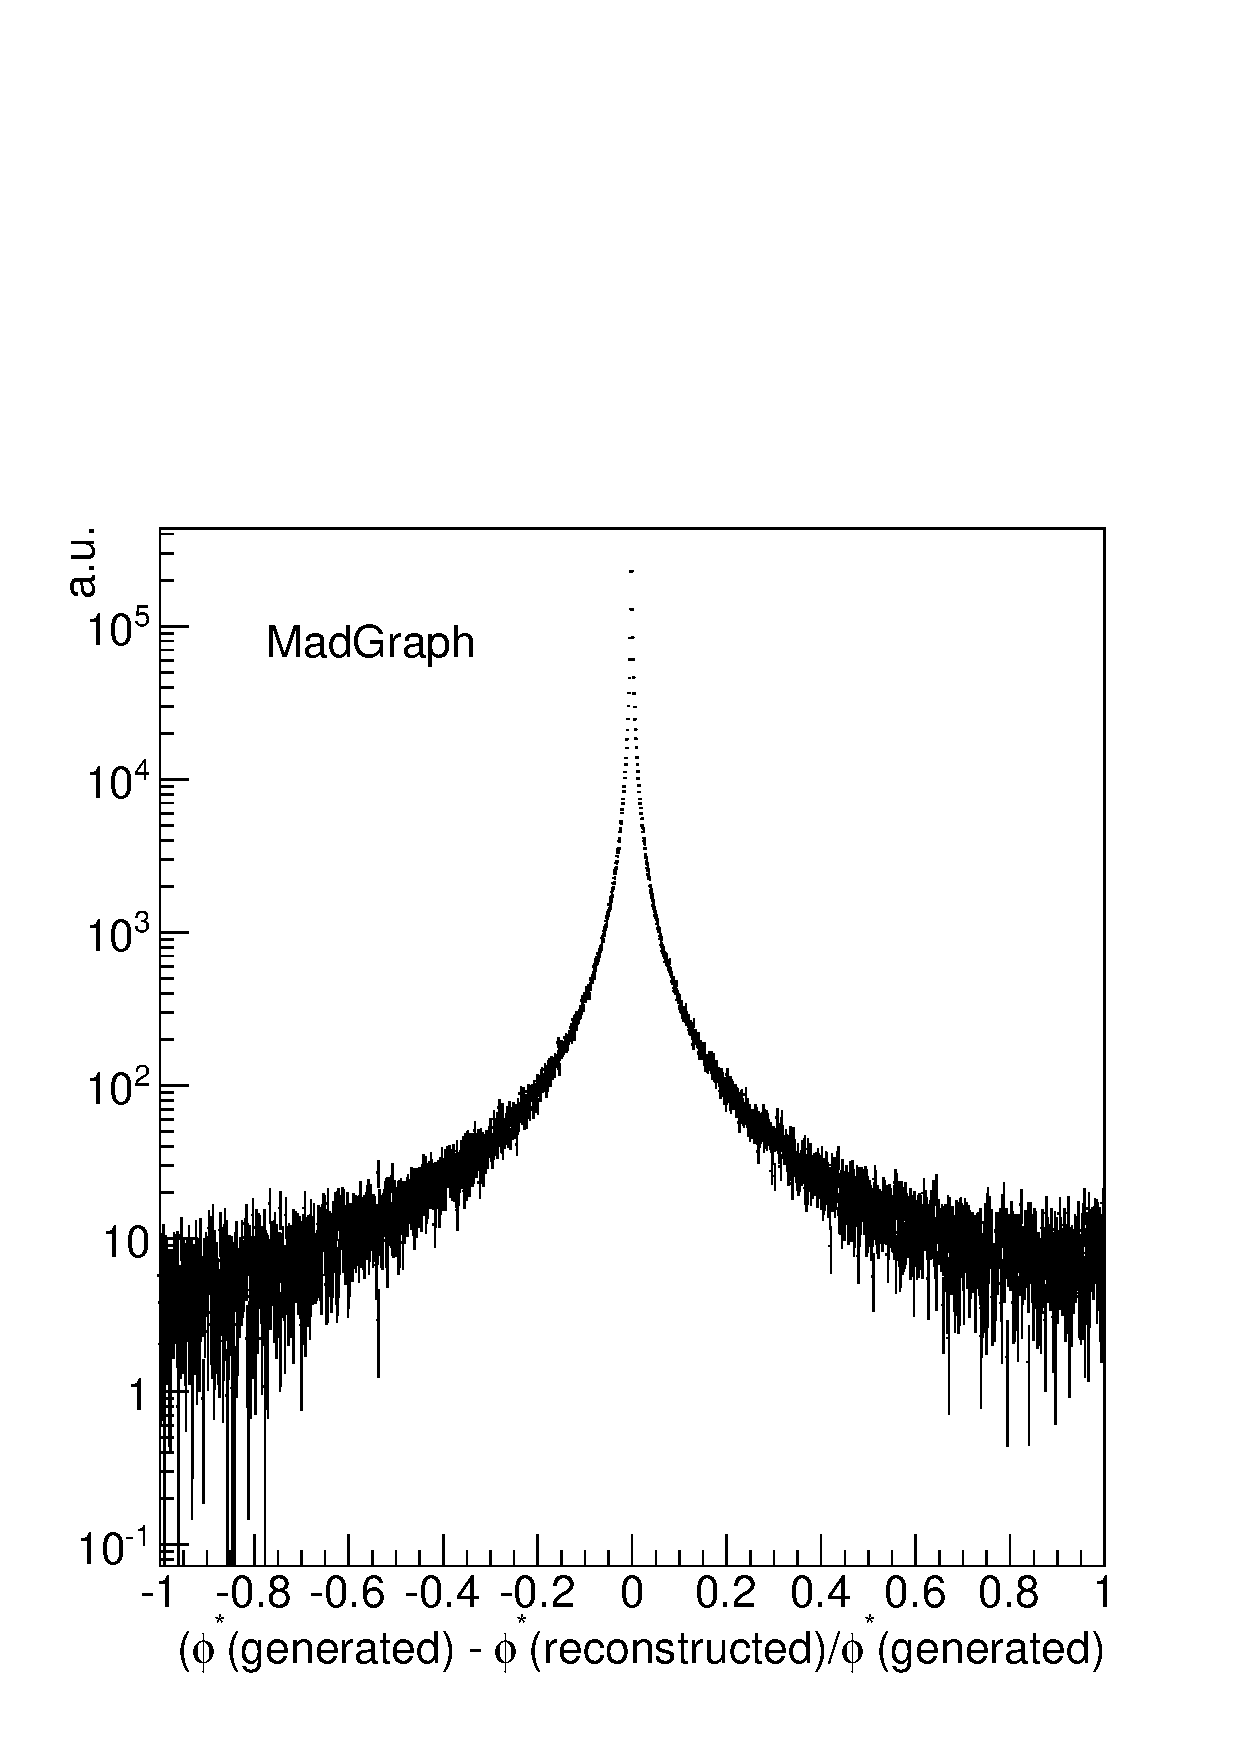
\includegraphics[width=\textwidth]{figures/DPhistar_M.pdf}
        \caption{}
        \label{fig:phistar_resolution}
    \end{subfigure}% Make side by side
    \begin{subfigure}[b]{\SideBySidePlotWidth}
        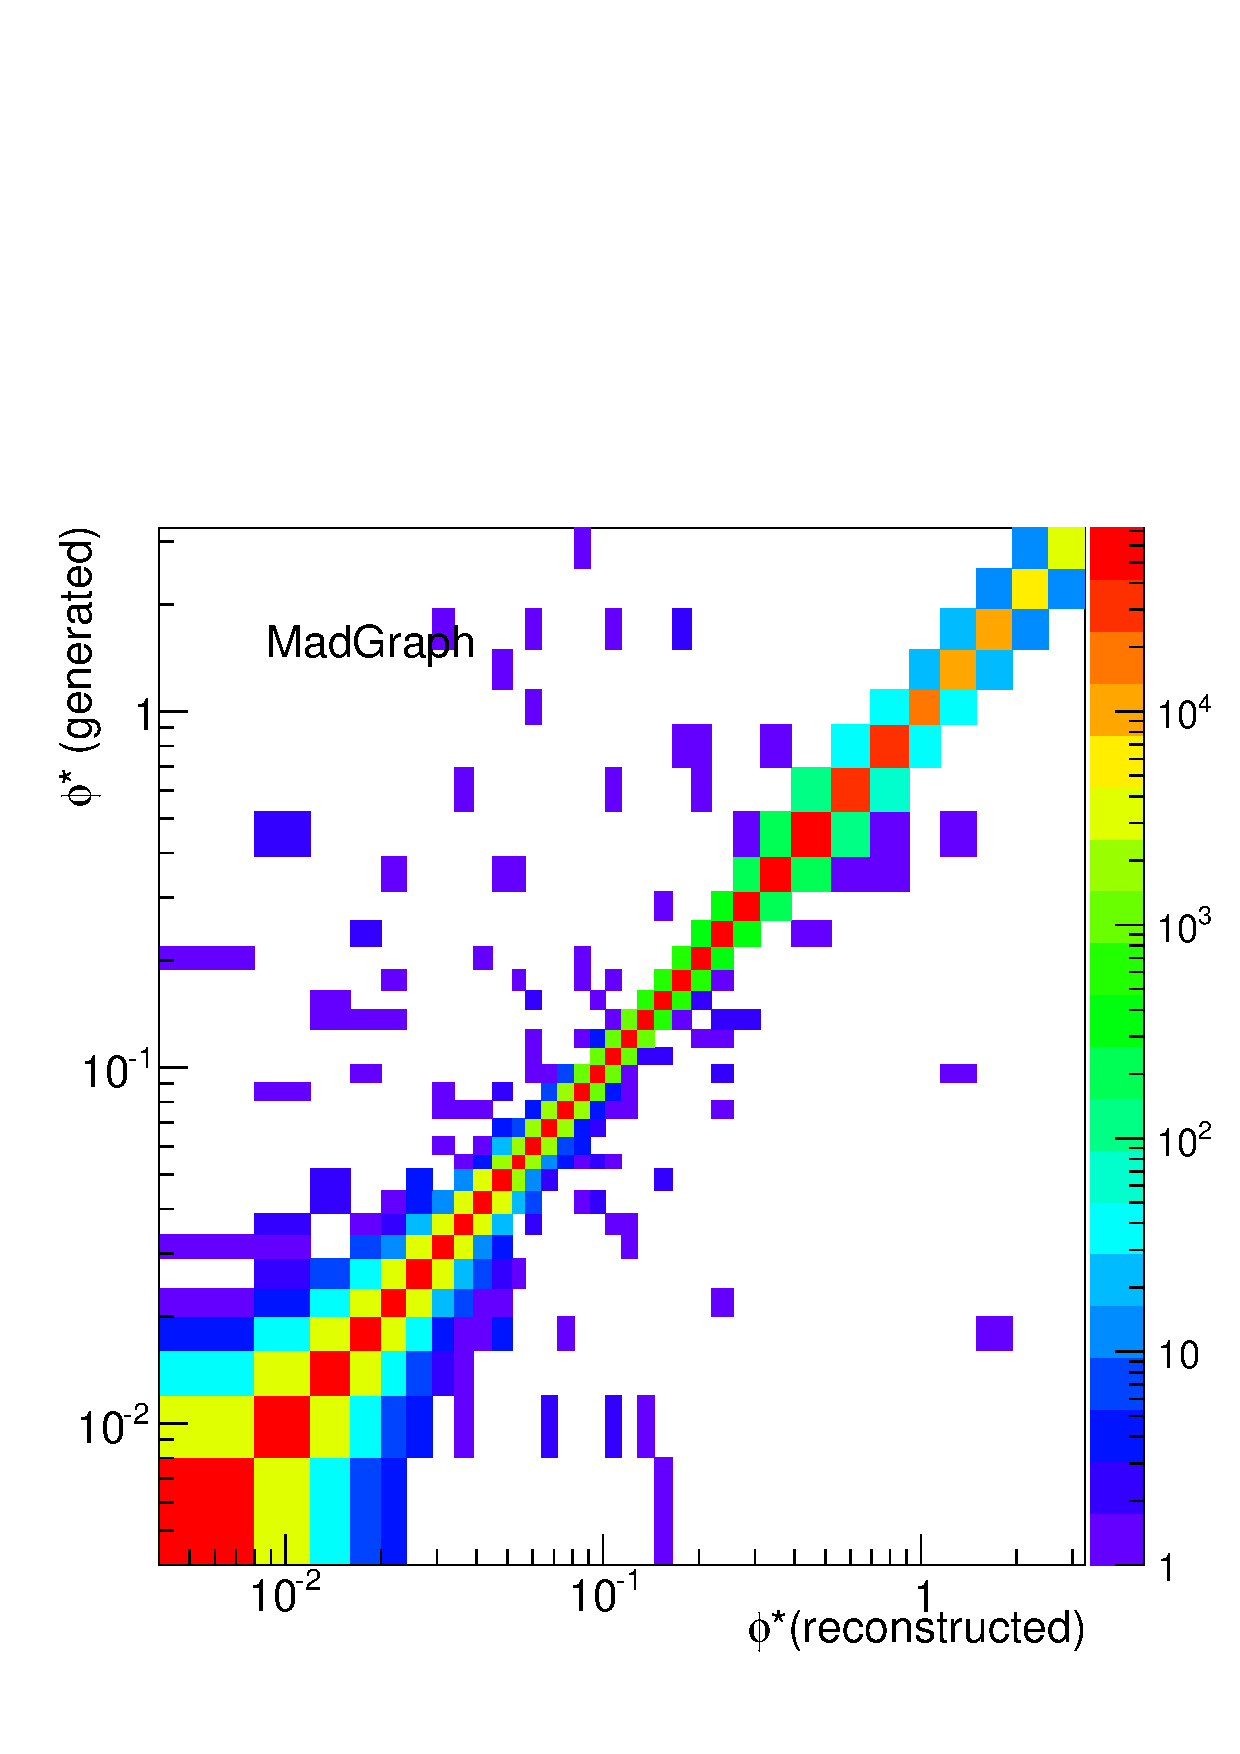
\includegraphics[width=\textwidth]{figures/BinM_M.pdf}
        \caption{}
        \label{fig:bin_migration_matrix}
    \end{subfigure}
    \caption{
        The \phistar reconstruction resolution (left) and bin migration (right)
        in \Ztoee events generated with \MADGRAPH passing our event selection.
    }
    \label{fig:phistar_resolution_and_bin_migration}
\end{figure}

\RooUnfold is used to perform the unfolding \cite{adye_2011}. It implements
Bayes' theorem as described in \cite{dagostini_1995}, and iteratively applies
it to invert the response matrix. \RooUnfold uses a limited number of
iterations in order to terminate the algorithm before finding the true (but
highly unstable) inverse. Four iterations are used in this analysis.

\subsubsection{Closure Tests}

This unfolding procedure was tested in several ways using the two signal MC
samples discussed in \SEC~\ref{ssec:monte_carlo}. First, the reconstructed
\phistar distributions from the \MADGRAPH and \POWHEG sample were unfolded
using their own generator level quantities and compared to their generator
level \phistar distributions.
The result of this test for \MADGRAPH is shown
in \FIG~\ref{fig:unfolding_madgraph_with_madgraph}, while the result for
\POWHEG is shown in \FIG~\ref{fig:unfolding_powheg_with_powheg}.

\begin{figure}[!htbp]
    \centering
    \begin{subfigure}[b]{\SideBySidePlotWidth}
        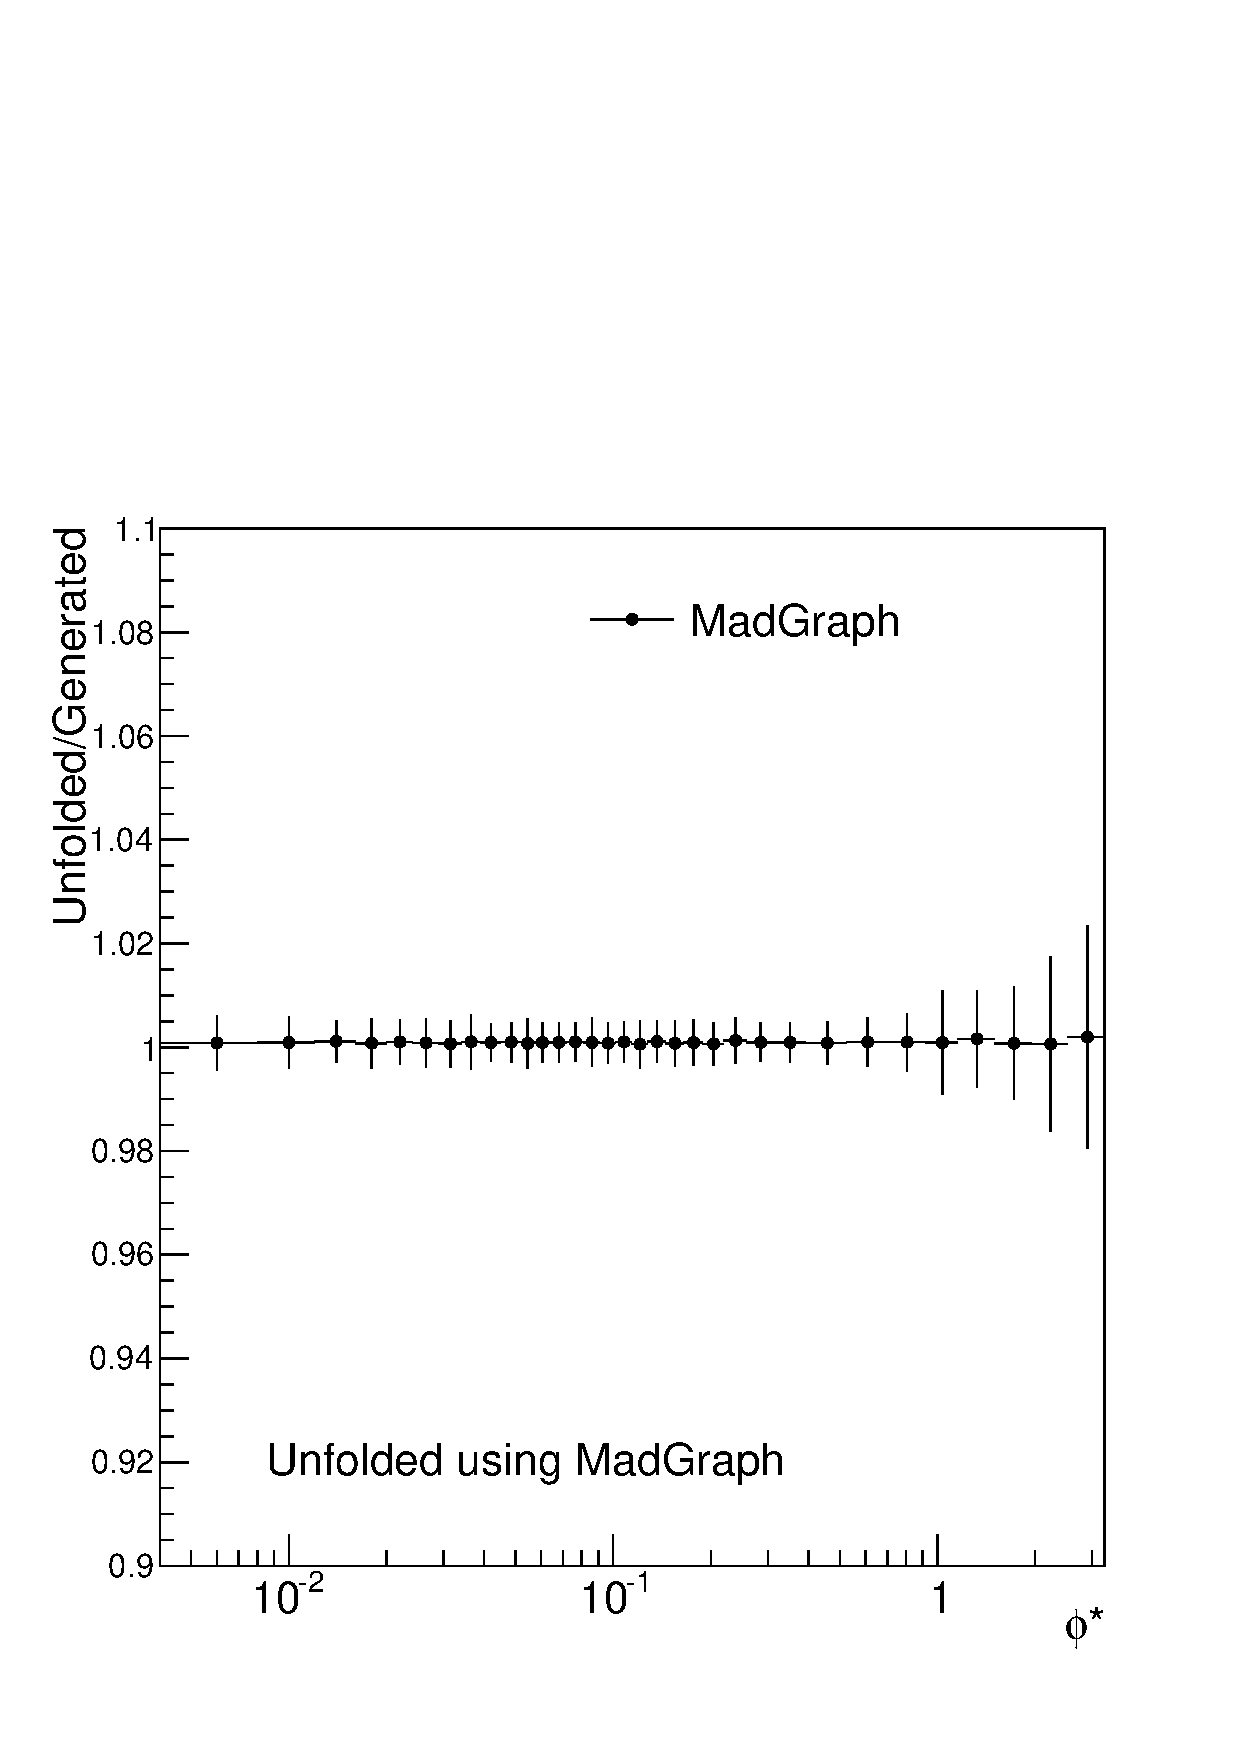
\includegraphics[width=\textwidth]{figures/BinM_MM.pdf}
        \caption{}
        \label{fig:unfolding_madgraph_with_madgraph}
    \end{subfigure}% Make side by side
    \begin{subfigure}[b]{\SideBySidePlotWidth}
        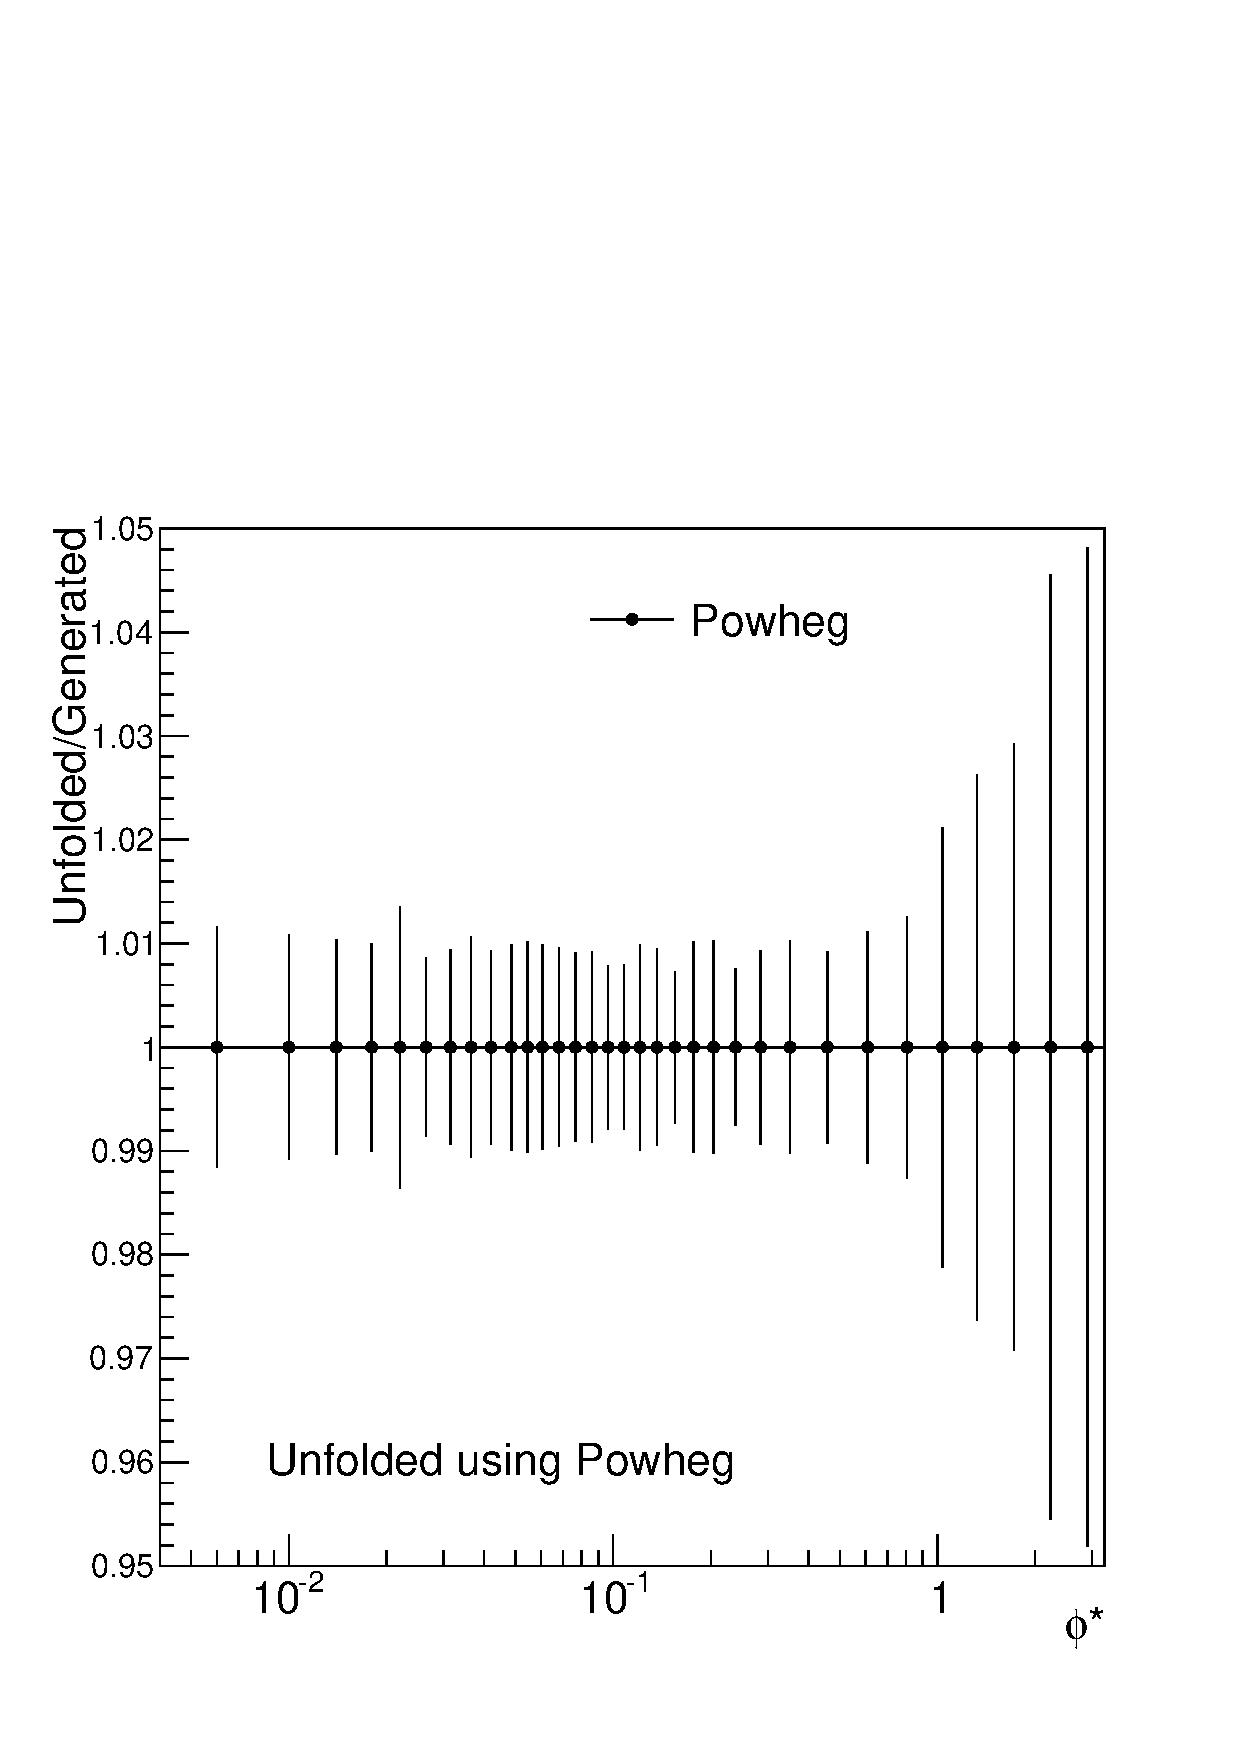
\includegraphics[width=\textwidth]{figures/BinM_PP.pdf}
        \caption{}
        \label{fig:unfolding_powheg_with_powheg}
    \end{subfigure}
    \caption{
        The ratio between the unfolded reconstructed \phistar distribution
        and the true generated \phistar distribution in \Ztoee
        events generated with \MADGRAPH (left) and \POWHEG (right) for events
        passing our event selection. The unfolding was done with the same
        \MADGRAPH (left) and \POWHEG (right) sample.
    }
    \label{fig:unfolded_vs_true_in_mc}
\end{figure}

Second, each MC signal sample was also divided into two independent halves. The
reconstructed \phistar distribution in each half was unfolded using the
generator level quantities from the other half. The two halves were then
compared to each other. The result of this test for \MADGRAPH is shown in
\FIG~\ref{fig:unfolding_madgraph_with_madgraph_halves}, while the result for
\POWHEG is shown in \FIG~\ref{fig:unfolding_powheg_with_powheg_halves}.

\begin{figure}[!htbp]
    \centering
    \begin{subfigure}[b]{\SideBySidePlotWidth}
        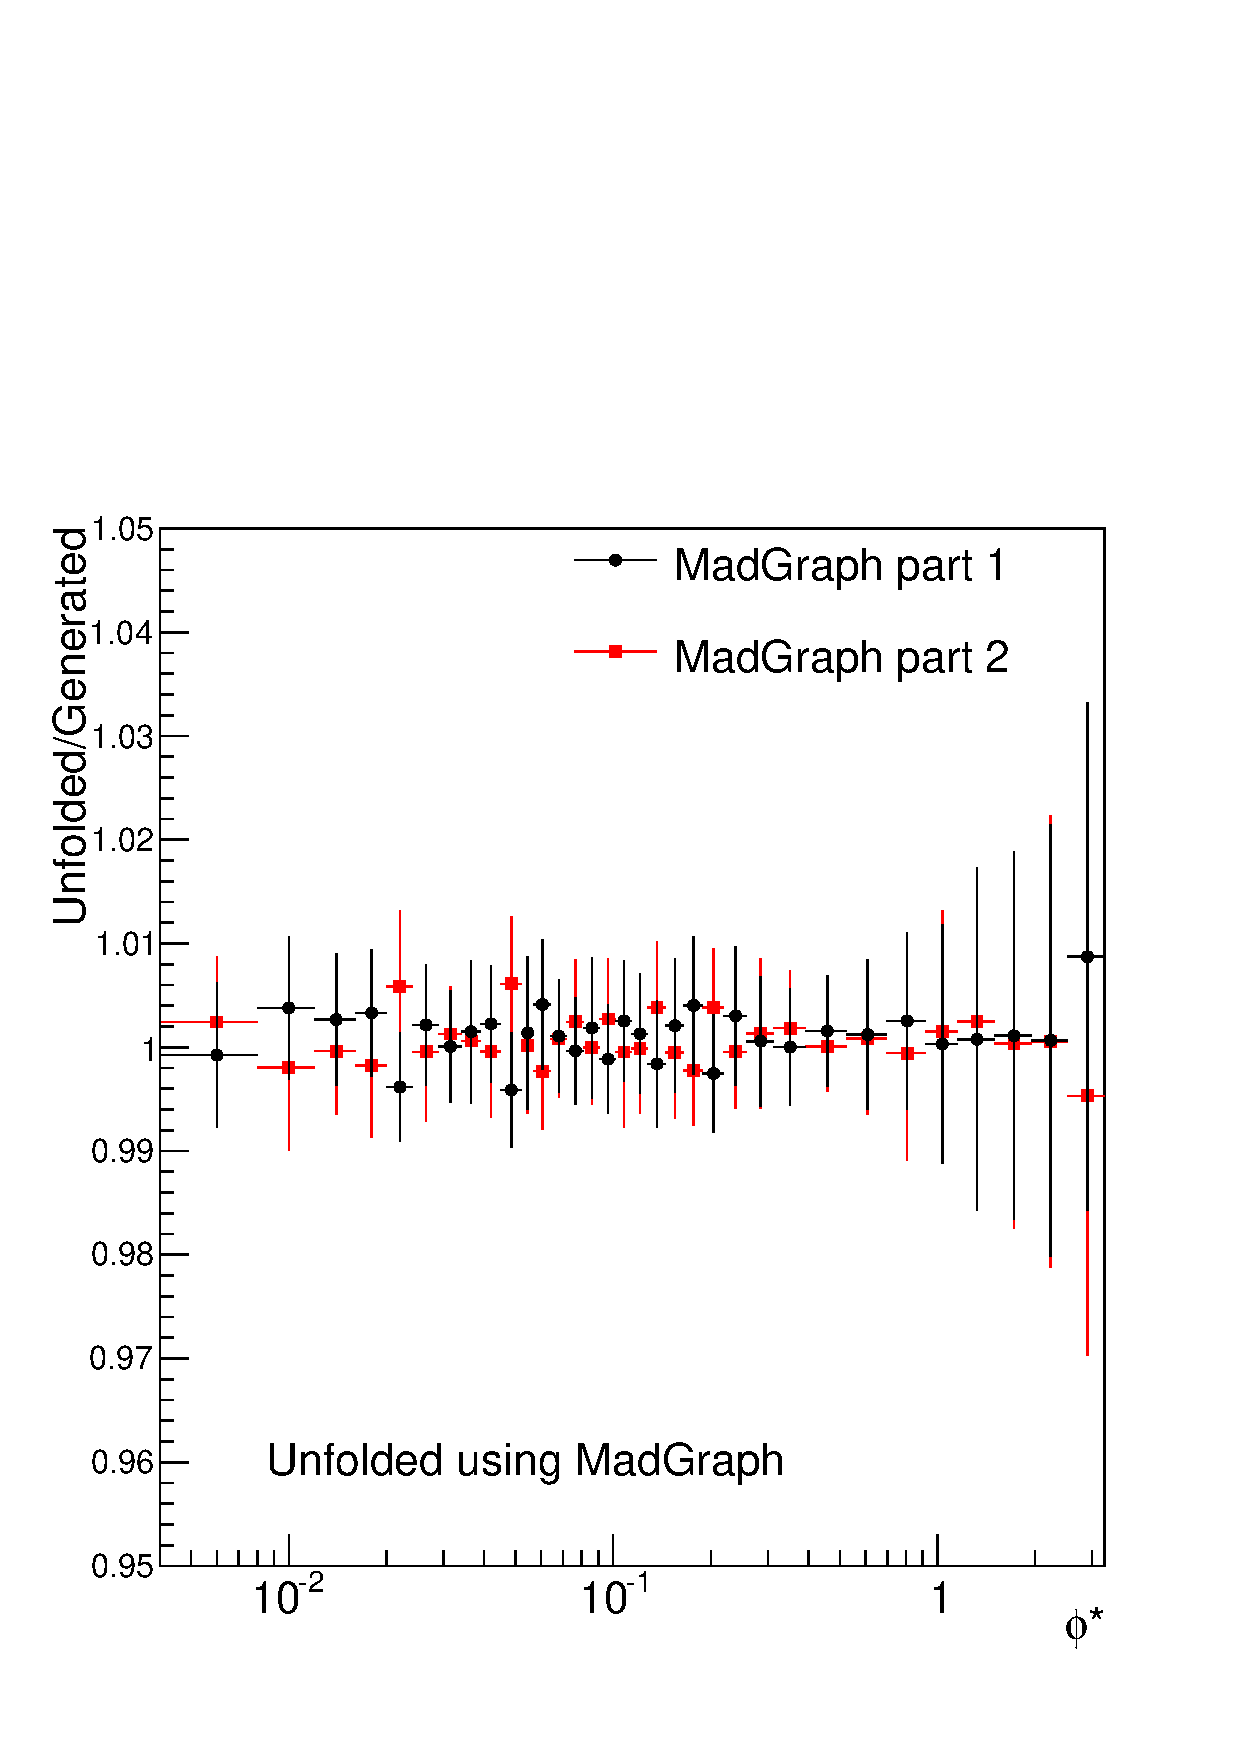
\includegraphics[width=\textwidth]{figures/BinM_M1M2.pdf}
        \caption{}
        \label{fig:unfolding_madgraph_with_madgraph_halves}
    \end{subfigure}% Make side by side
    \begin{subfigure}[b]{\SideBySidePlotWidth}
        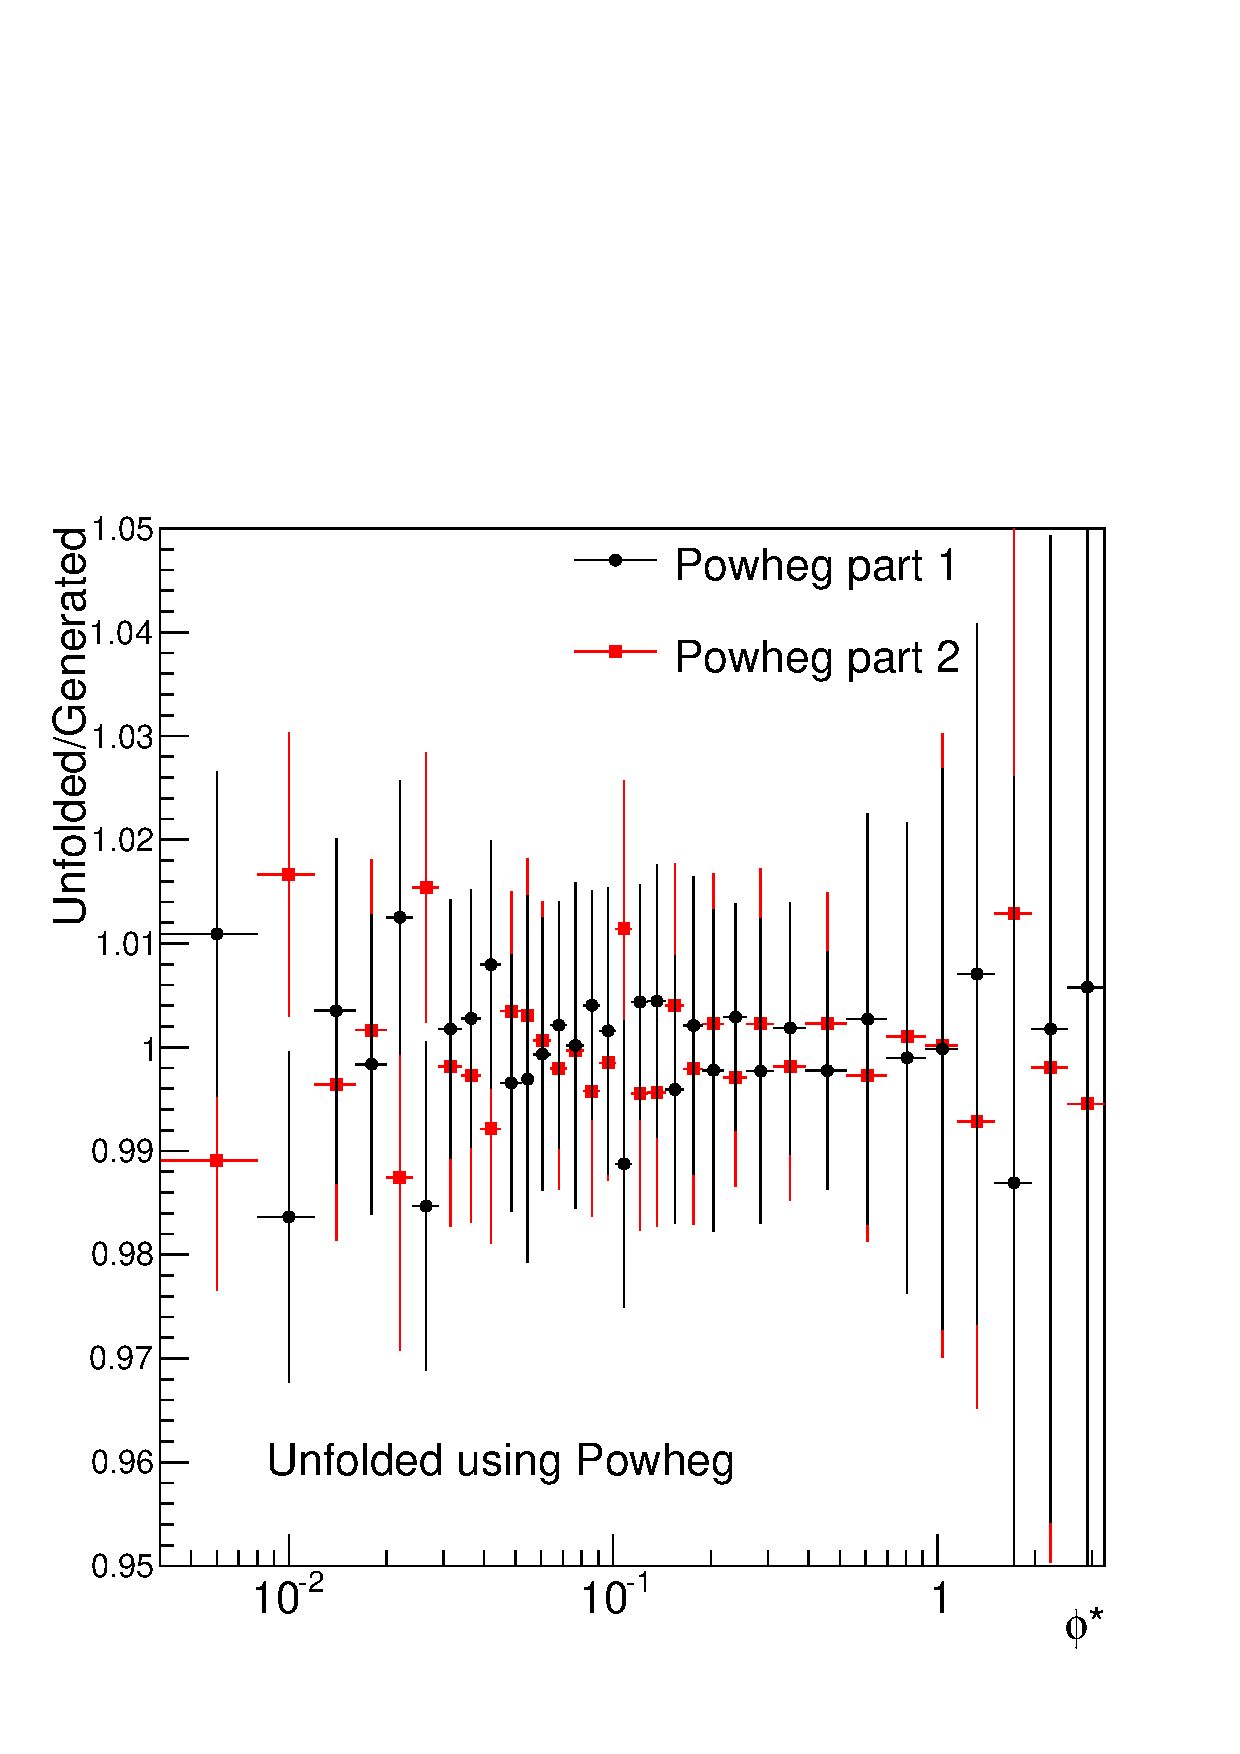
\includegraphics[width=\textwidth]{figures/BinM_P1P2.pdf}
        \caption{}
        \label{fig:unfolding_powheg_with_powheg_halves}
    \end{subfigure}
    \caption{
        The ratio between the unfolded reconstructed \phistar distribution and
        the true generated \phistar distribution in two (circular and square
        points) statistically independent samples of \Ztoee events generated
        with \MADGRAPH (left) and \POWHEG (right) for events passing our event
        selection. Each reconstructed \phistar distribution was unfolded using
        the statistically independent sample produced by the same generator.
    }
    \label{fig:half_vs_half_unfolding}
\end{figure}

Third and finally, the reconstructed \phistar distribution from the \MADGRAPH
sample was unfolded with the generator level quantities from the \POWHEG sample
and vice versa. The result of unfolding \POWHEG with \MADGRAPH is shown in
\FIG~\ref{fig:unfolding_powheg_with_madgraph}, while the result of unfolding
\MADGRAPH with \POWHEG is shown in
\FIG~\ref{fig:unfolding_madgraph_with_powheg}.

\begin{figure}[!htbp]
    \centering
    \begin{subfigure}[b]{\SideBySidePlotWidth}
        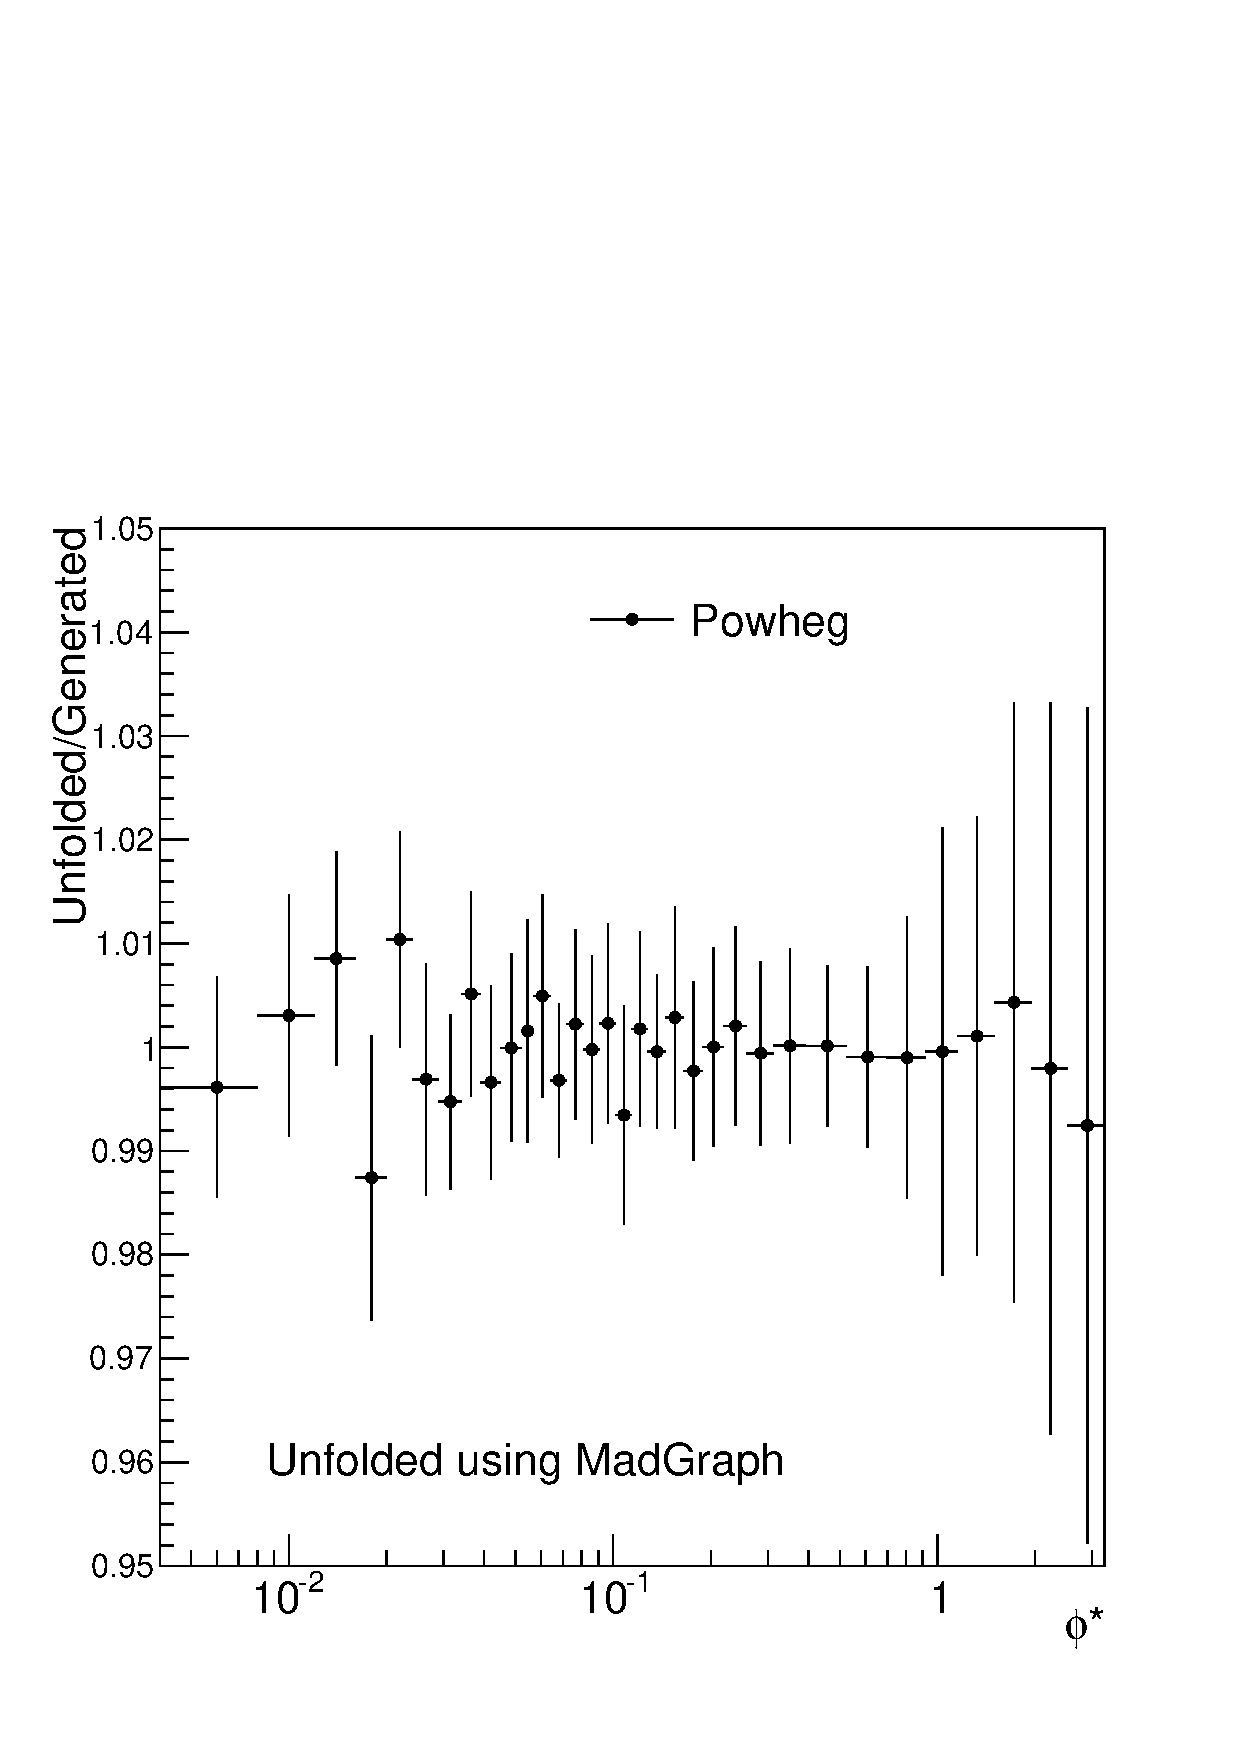
\includegraphics[width=\textwidth]{figures/BinM_MP.pdf}
        \caption{}
        \label{fig:unfolding_powheg_with_madgraph}
    \end{subfigure}% Make side by side
    \begin{subfigure}[b]{\SideBySidePlotWidth}
        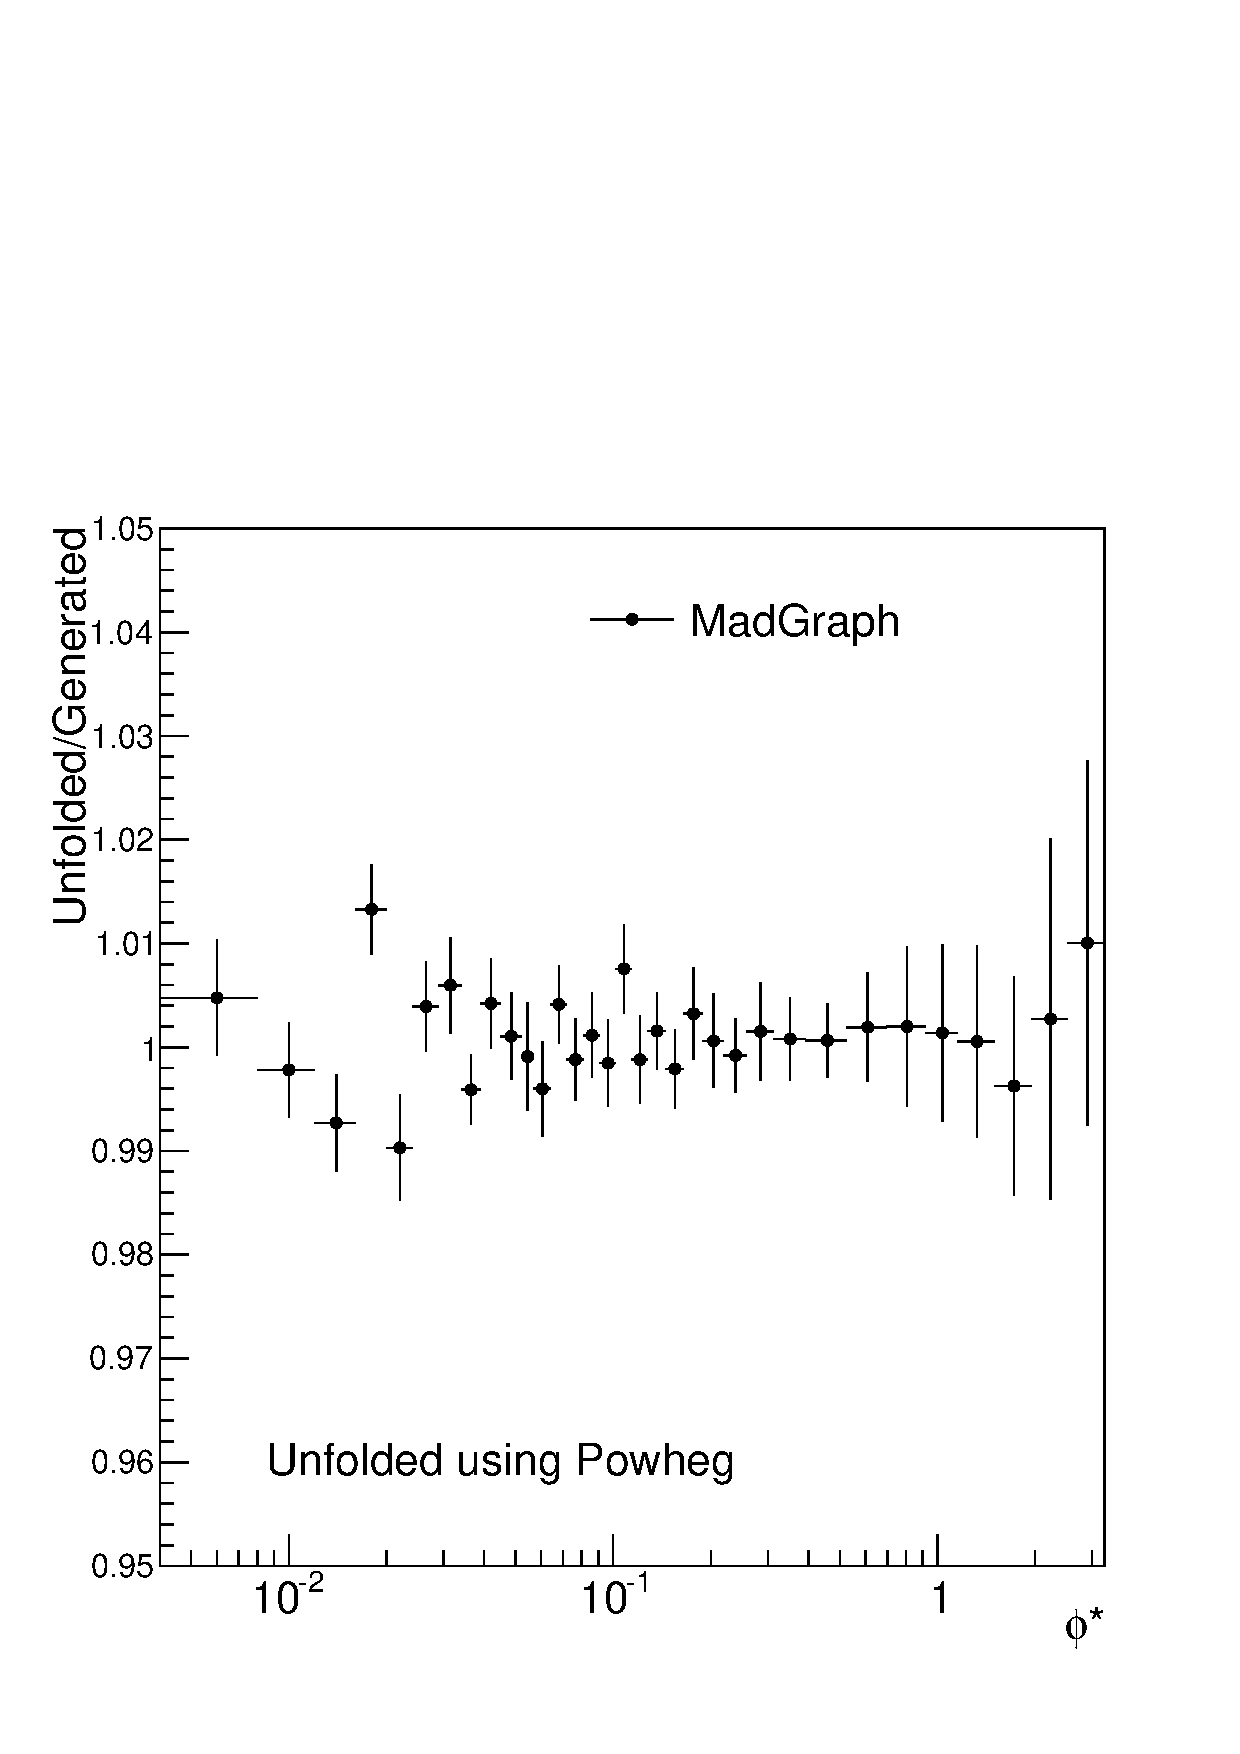
\includegraphics[width=\textwidth]{figures/BinM_PM.pdf}
        \caption{}
        \label{fig:unfolding_madgraph_with_powheg}
    \end{subfigure}
    \caption{
        The ratio between the unfolded reconstructed \phistar distribution and
        the true generated \phistar distribution in \Ztoee events generated
        with \POWHEG (left) and \MADGRAPH (right) for events passing our event
        selection. The unfolding was done with the \MADGRAPH (left) and \POWHEG
        (right) sample.
    }
    \label{fig:cross_mc_unfolding}
\end{figure}

In most cases the results are consistent within the assigned statistical error
bars. However, in the case of the \MADGRAPH sample unfolded with \POWHEG, there
is disagreement between in the low \phistar bins. This is due \RooUnfold under
estimating the uncertainties, as discussed in
\SEC~\ref{ssec:unfolding_statistical_uncertainties}.

\subsubsection{Statistical Uncertainties}
\label{ssec:unfolding_statistical_uncertainties}

The uncertainties shown in \FIGS~\ref{fig:unfolded_vs_true_in_mc},
\ref{fig:half_vs_half_unfolding}, and \ref{fig:cross_mc_unfolding} are the
statistical uncertainties returned by \RooUnfold. These uncertainties only take
the number of events in the reconstructed distribution into account. The
uncertainties are correlated by the off-diagonal elements. While \RooUnfold can
return the full covariance matrix, we instead use a simpler approximation
provided by \RooUnfold where the uncertainties are based only on the diagonal
elements. We tested the effects of this simplification on the uncertainties
using two tests discussed below.

In the first test, each bin in the \POWHEG \phistar distribution was
regenerated from a Gaussian with the value of the original bin as the mean and
the value of the statistical uncertainty on the bin from the original
distribution as the standard deviation. Using this process, \num{500} \phistar
distributions were generated, giving us \num{501} total distributions as the
original distribution was also used. These distributions were then unfolded
using the full \MADGRAPH sample. The results are shown in
\FIG~\ref{fig:toy_unfolding_results} where the square points are the median
value of the 501 distributions, and the error bars show the extent of the value
in the central 68.2\% of the distributions. These are compared to the errors
provided by \RooUnfold. Both methods lead to identical results.

\begin{figure}[!htbp]
    \centering
    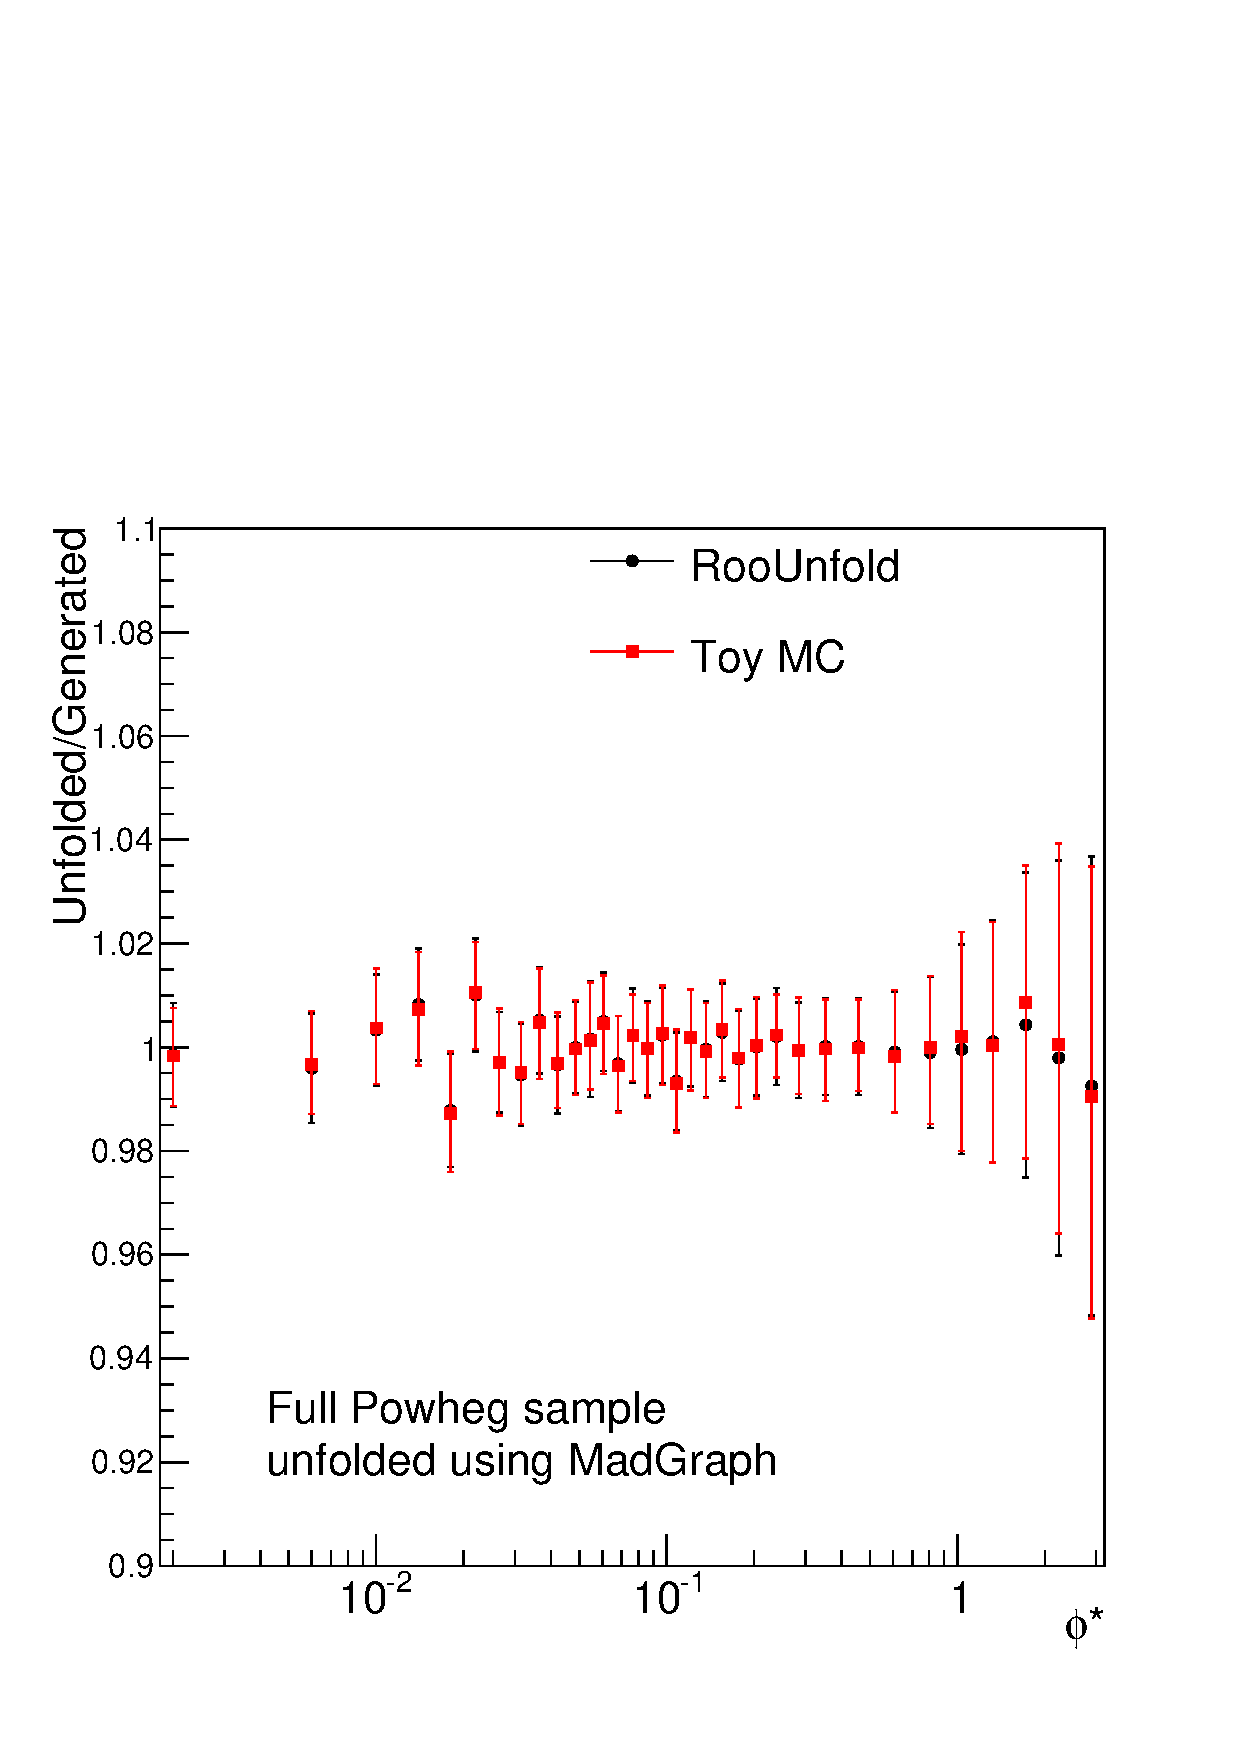
\includegraphics[width=\SideBySidePlotWidth]{figures/BinM_MP_ALL.pdf}
    \caption{
        The ratio between the unfolded reconstructed \phistar distribution and
        the true generated \phistar distribution for \Ztoee events generated
        with \POWHEG. The unfolding was done with the \MADGRAPH sample. The
        distribution shown with circular points shows the results using the
        uncertainty propagation included in the \RooUnfold package. The
        distribution shown with square points is obtained by unfolding 500 toy
        MC variations of the reconstructed \phistar distribution.
    }
    \label{fig:toy_unfolding_results}
\end{figure}

In the second test, \num{5000} and \num{50000} randomly selected events from
the \POWHEG sample were used instead of the data, and 501 distributions were
constructed in the same manner as above. The results of the test with
\num{5000} events is shown in \FIG~\ref{fig:unfolding_5000}, while the result
of the test with \num{50000} events is shown in \FIG~\ref{fig:unfolding_50000}.
As expected, when fewer reconstructed events are used in the unfolding, the
uncertainties reported by \RooUnfold are larger. In both tests, the simplified
error handling produces the same results and so is used.

\begin{figure}[!htbp]
    \centering
    \begin{subfigure}[b]{\SideBySidePlotWidth}
        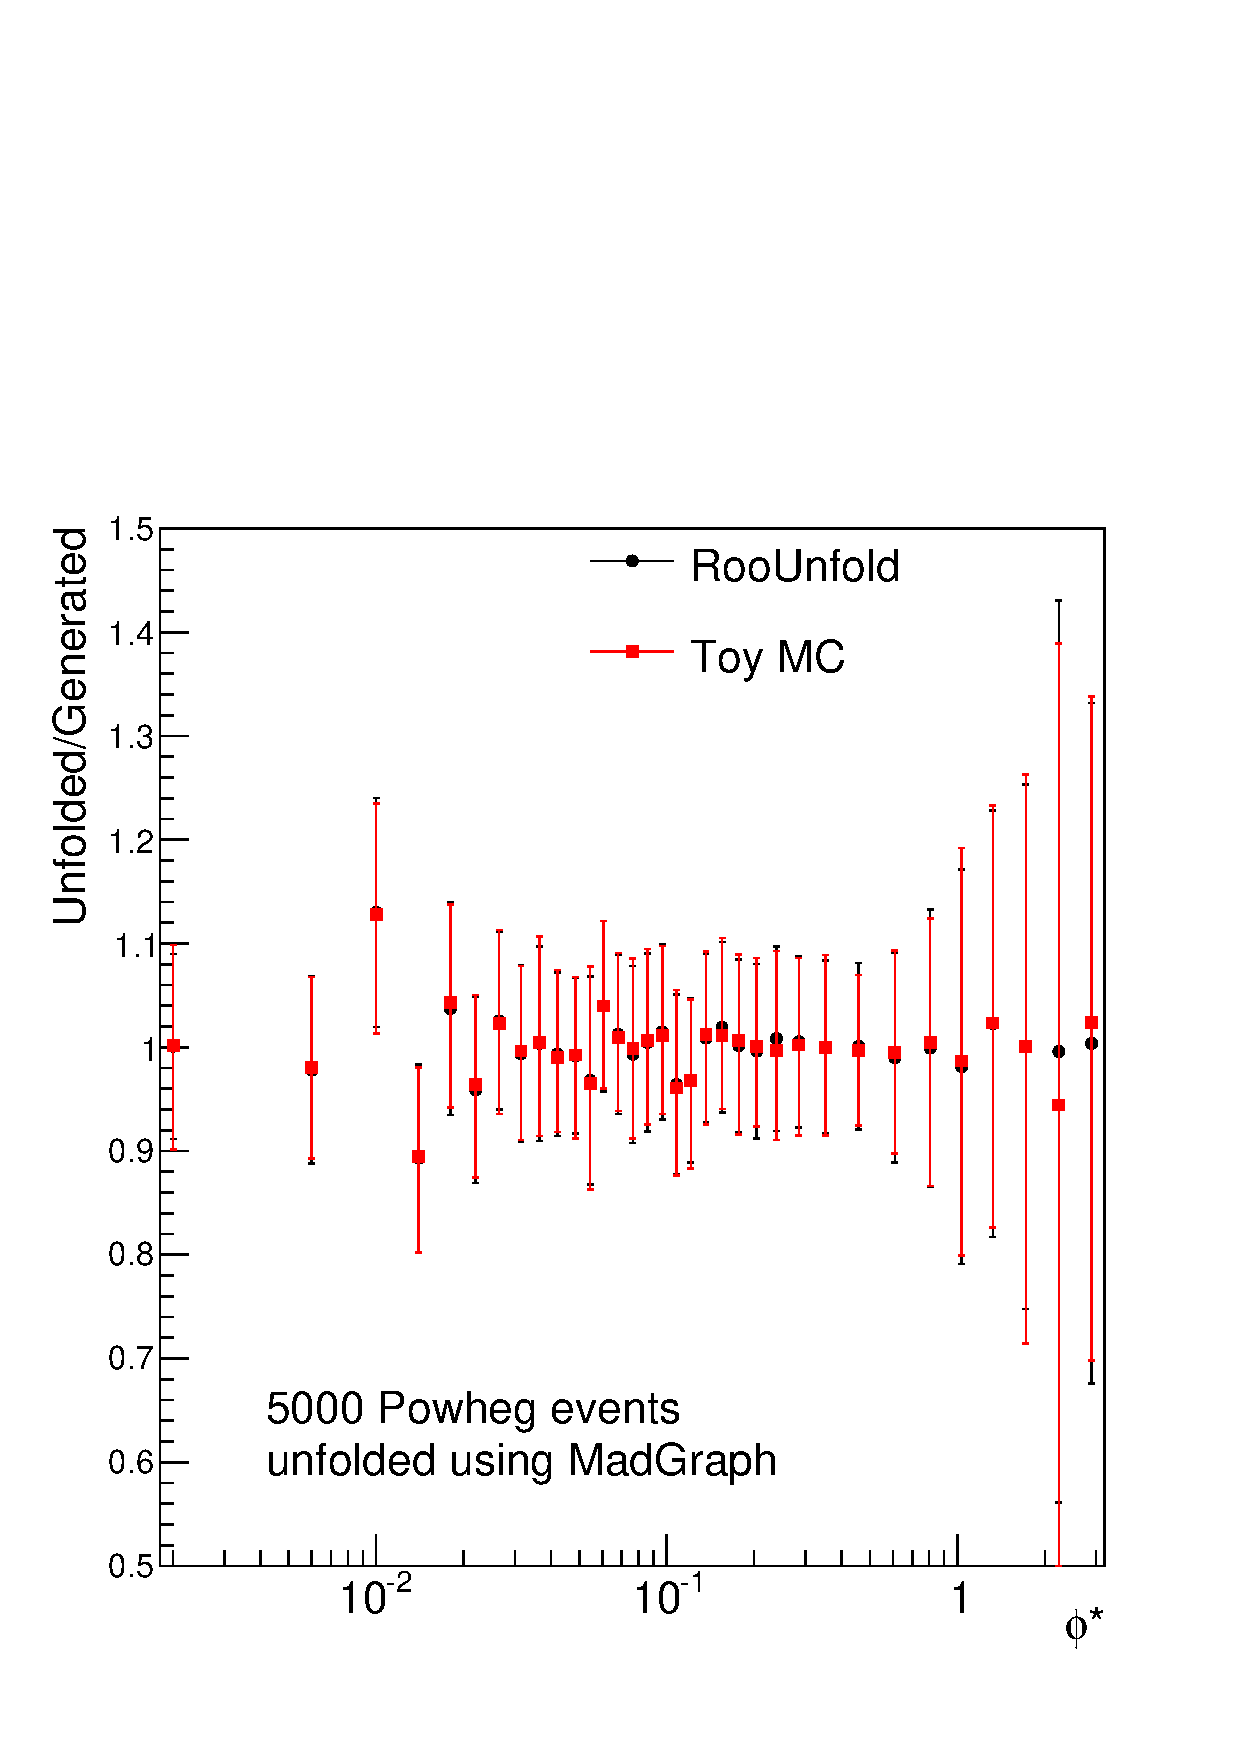
\includegraphics[width=\textwidth]{figures/BinM_MP_5000.pdf}
        \caption{}
        \label{fig:unfolding_5000}
    \end{subfigure}% Make side by side
    \begin{subfigure}[b]{\SideBySidePlotWidth}
        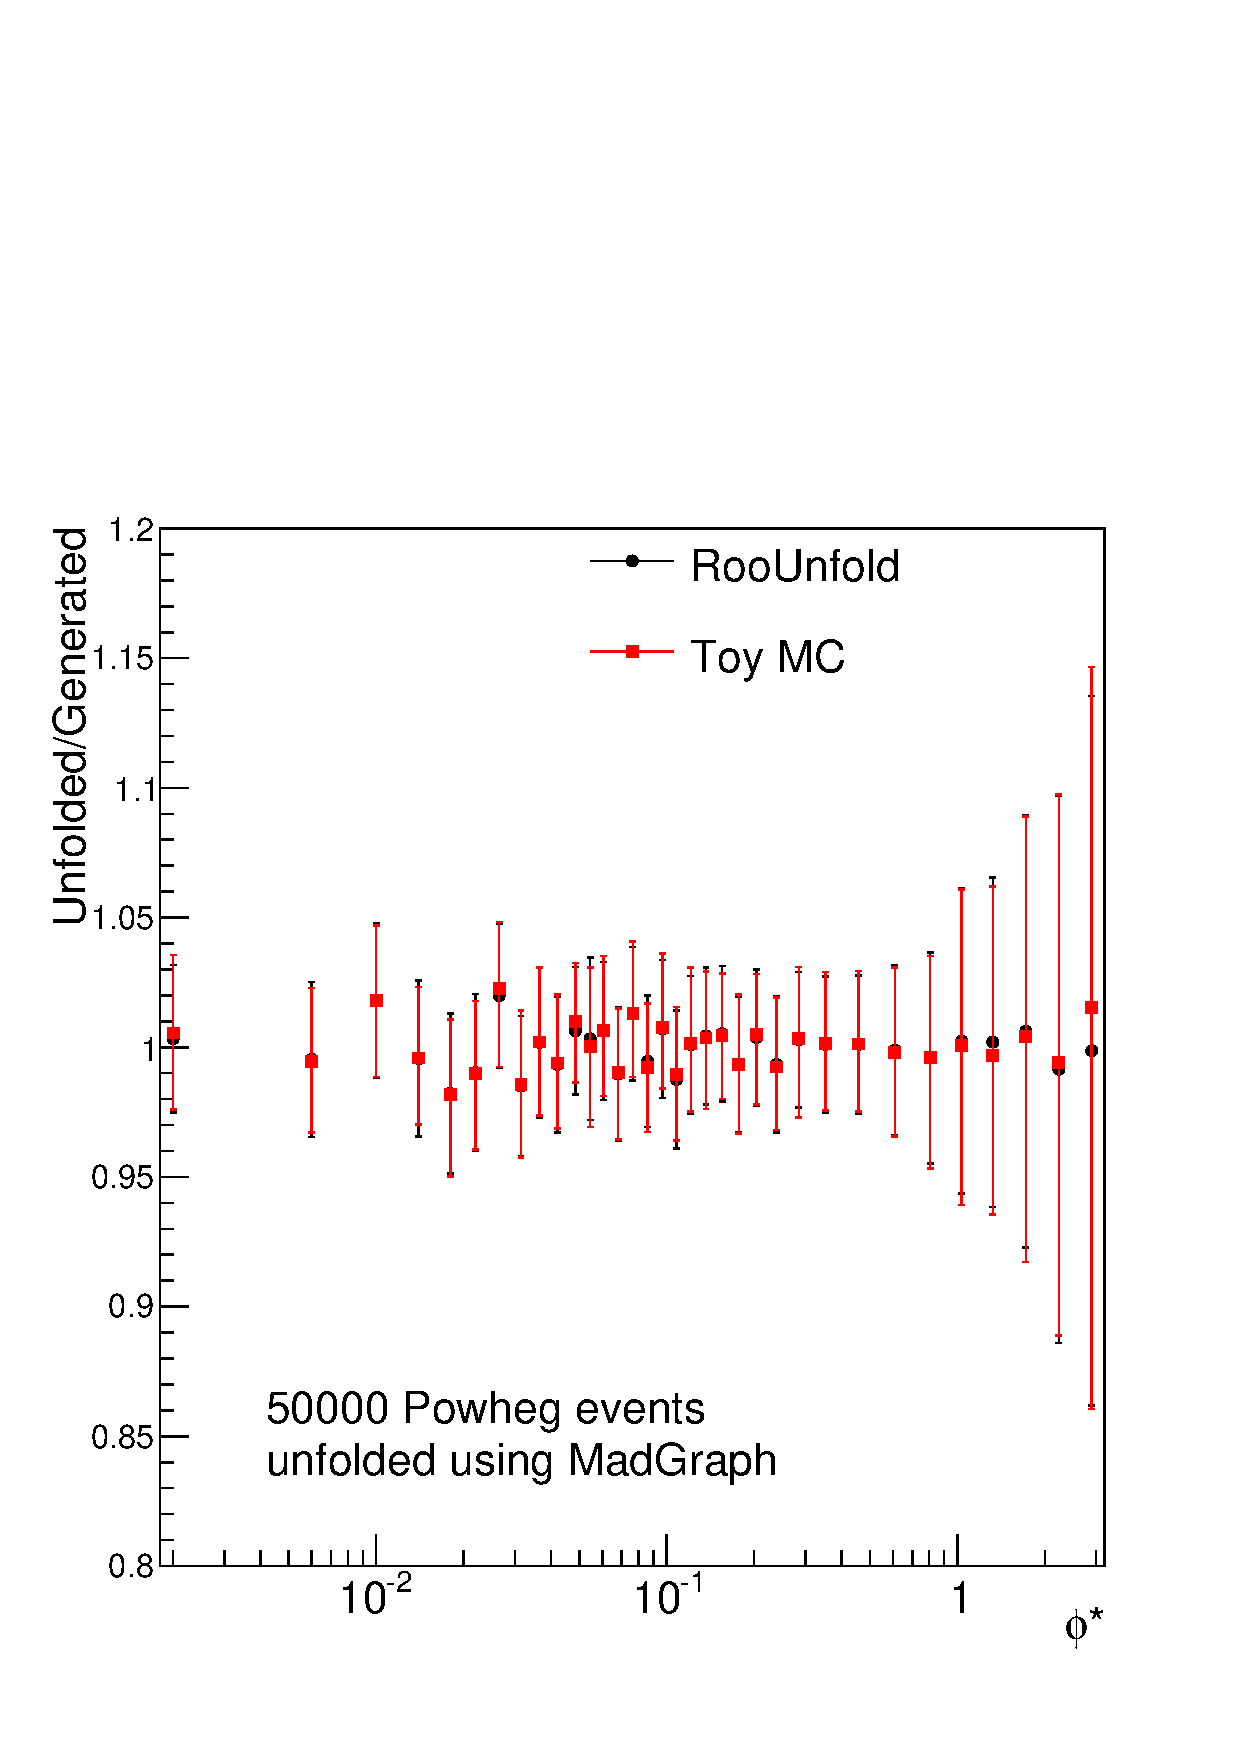
\includegraphics[width=\textwidth]{figures/BinM_MP_50000.pdf}
        \caption{}
        \label{fig:unfolding_50000}
    \end{subfigure}
    \caption{
        The ratio between the unfolded reconstructed \phistar distribution and
        the true generated \phistar distribution for \num{5000} (left) and
        \num{50000} (right) \Ztoee events generated with \POWHEG. The unfolding
        was done with the \MADGRAPH sample. The distribution shown with
        circular points shows the results using the uncertainty propagation
        included in the \RooUnfold package. The distribution shown with square
        points is obtained by unfolding 500 toy MC variations of the
        reconstructed \phistar distribution.
    }
    \label{fig:toy_powheg_unfolding_results}
\end{figure}

While \RooUnfold properly handles the statistical uncertainty due to the number
of events in the data being unfolded, it does not account for statistical
uncertainty due to the number of generator level events used to create the
bin migration matrix. This leads to an underestimation of the total uncertainty
which is especially pronounced in cases where the number of events in the
MC sample is smaller than the number of data events, as is the case in this
analysis.

A toy MC method is used to propagate the uncertainty from the bin migration
matrix to the unfolded distribution. In this method, \num{500} new bin
migration matrices are generated by randomly fluctuating each bin of the
original matrix generated using \num{5000} events from the \POWHEG sample. Bins
with \num{0} events are left at \num{0}. Bins with a small number of
events---where the number of events in the bin divided by the statistical
uncertainty is less than \num{5}---are fluctuated using a Poisson distribution
with the number of events in the original bin as the most probable value. All
other bins are fluctuated using a Gaussian with mean equal to the number of
events in the original bin and standard deviation equal to the statistical
uncertainty on the original bin. The reconstructed \phistar distribution from
the full \MADGRAPH sample is then unfolded with each of the \num{501} bin
migration matrices. The results are shown in
\FIG~\ref{fig:5000_propegation_unfolding}.
Figure~\ref{fig:unfolding_madgraph_with_5000} shows the uncertainties from
\RooUnfold as compared to the uncertainties derived using the toy MC method.
Figure~\ref{fig:toy_mc_5000} shows the extent of the \phistar bin values
generated by the ensemble of toy MC bin migration matrices.
Figure~\ref{fig:pull_5000} shows the pull of the bins in
\FIG~\ref{fig:unfolding_madgraph_with_5000}.
Figure~\ref{fig:bin_migration_5000} shows the original bin migration matrix.

\begin{figure}[!htbp]
    \centering
    \begin{subfigure}[b]{\SideBySidePlotWidth}
        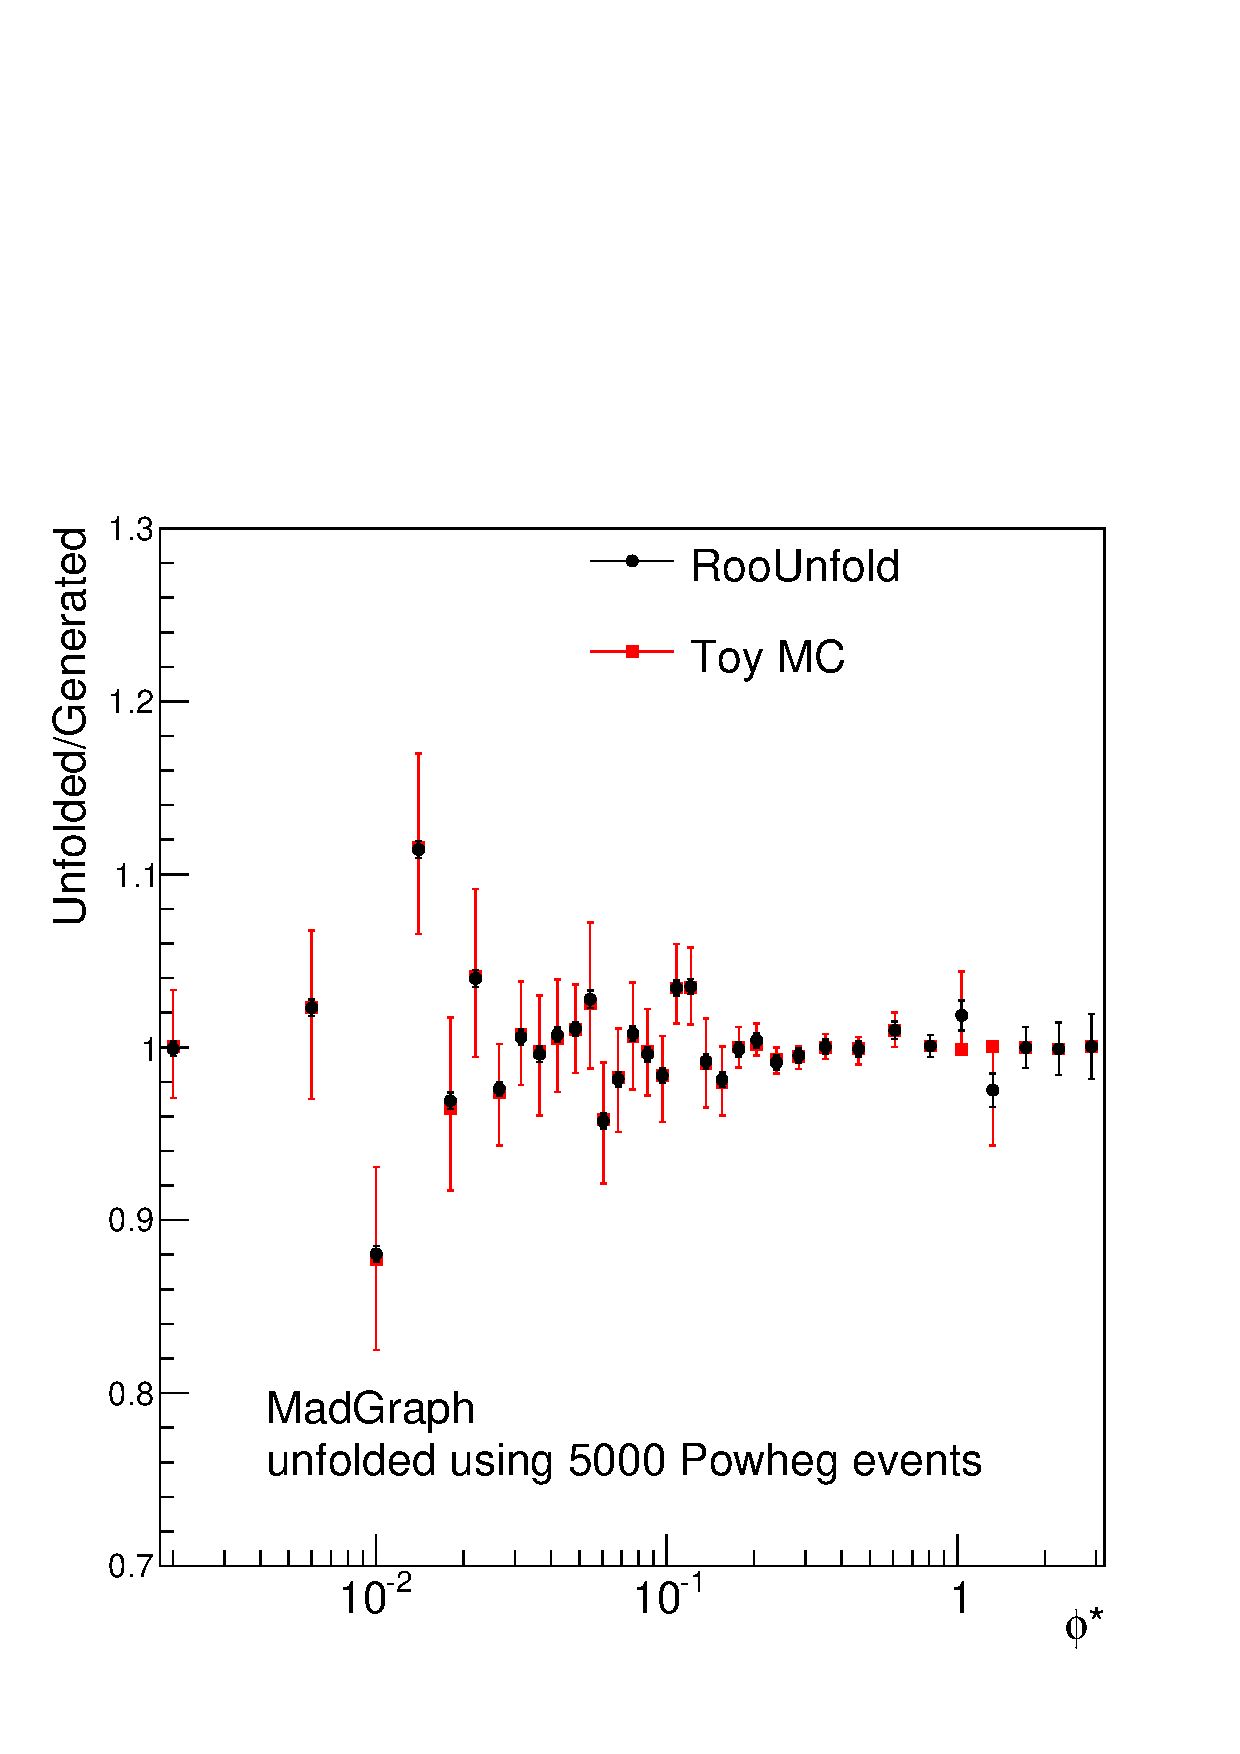
\includegraphics[width=\textwidth]{figures/BinM_PM_5000.pdf}
        \caption{}
        \label{fig:unfolding_madgraph_with_5000}
    \end{subfigure}% Make side by side
    \begin{subfigure}[b]{\SideBySidePlotWidth}
        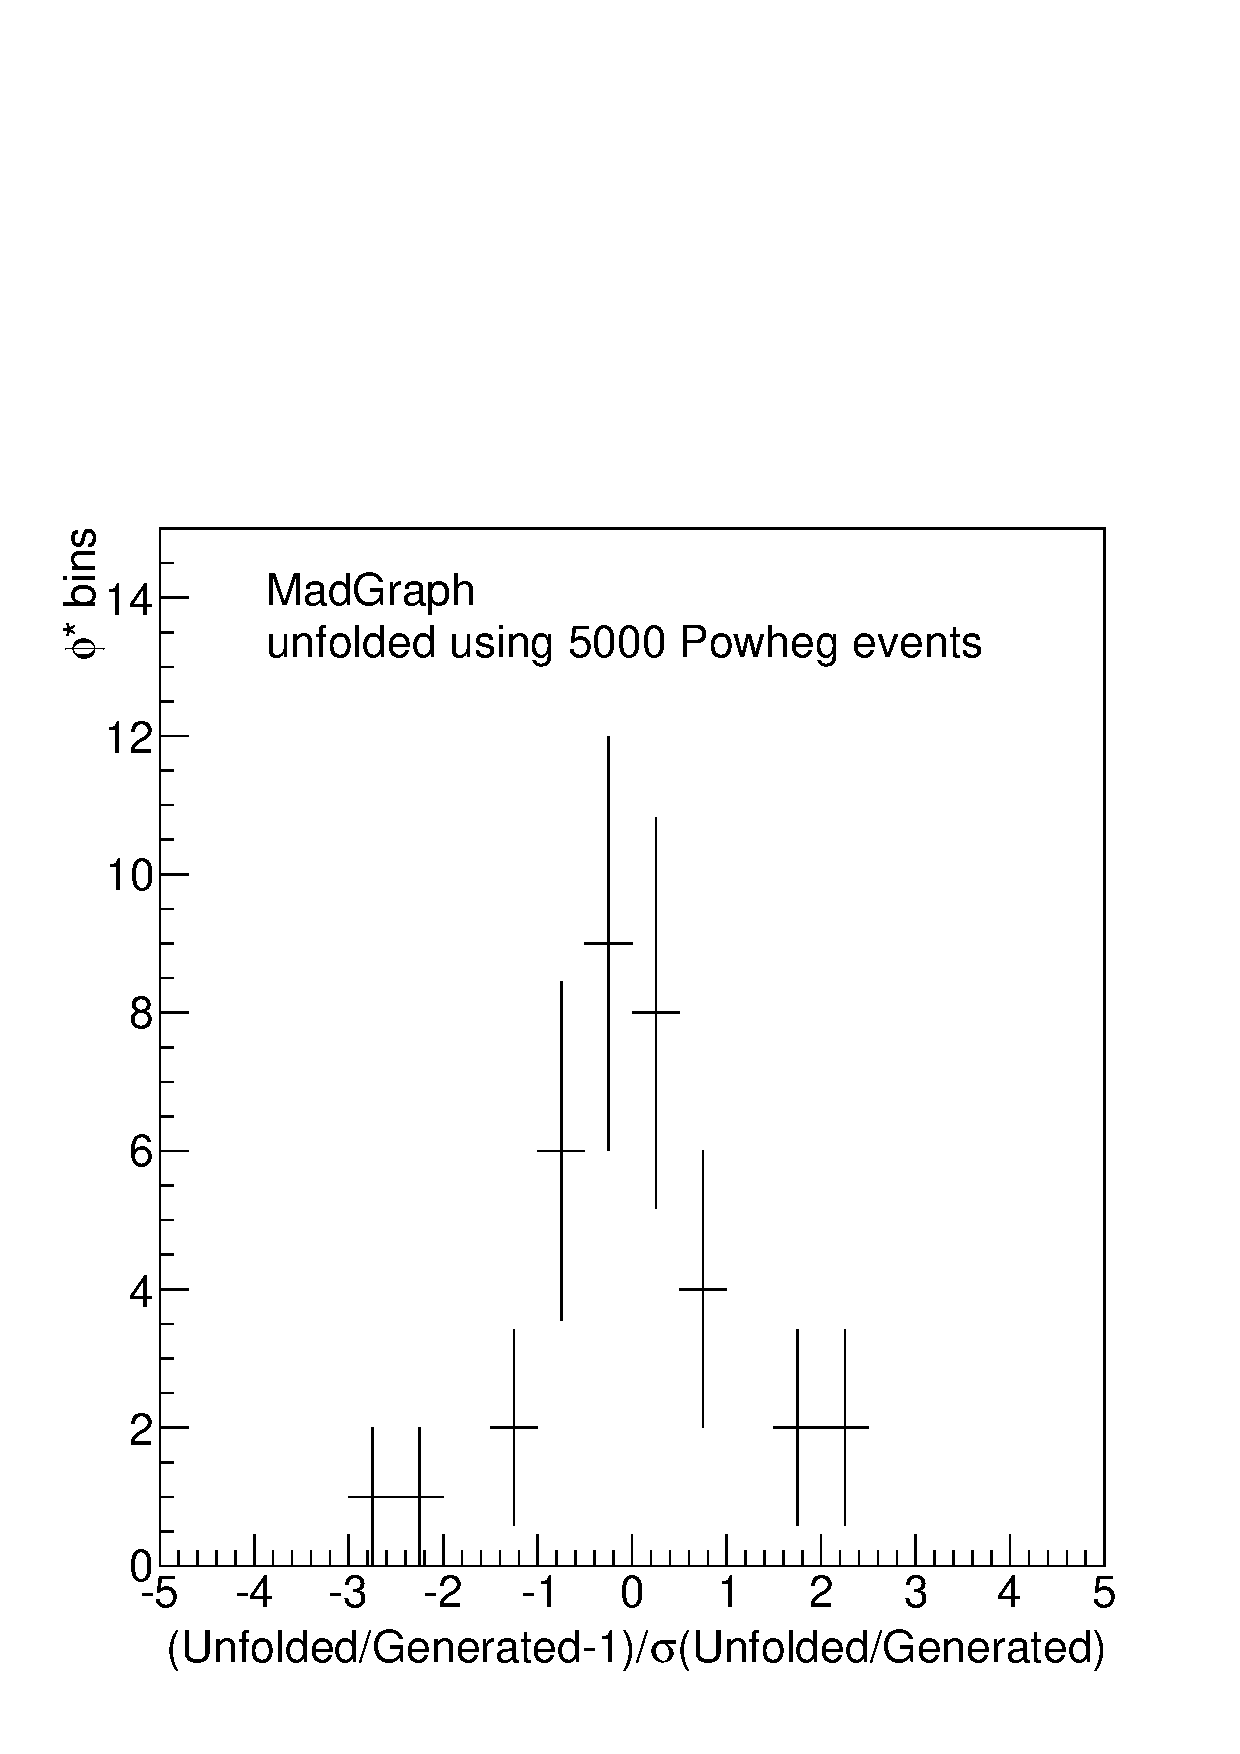
\includegraphics[width=\textwidth]{figures/Pull_5000.pdf}
        \caption{}
        \label{fig:pull_5000}
    \end{subfigure}
    \begin{subfigure}[b]{\SideBySidePlotWidth}
        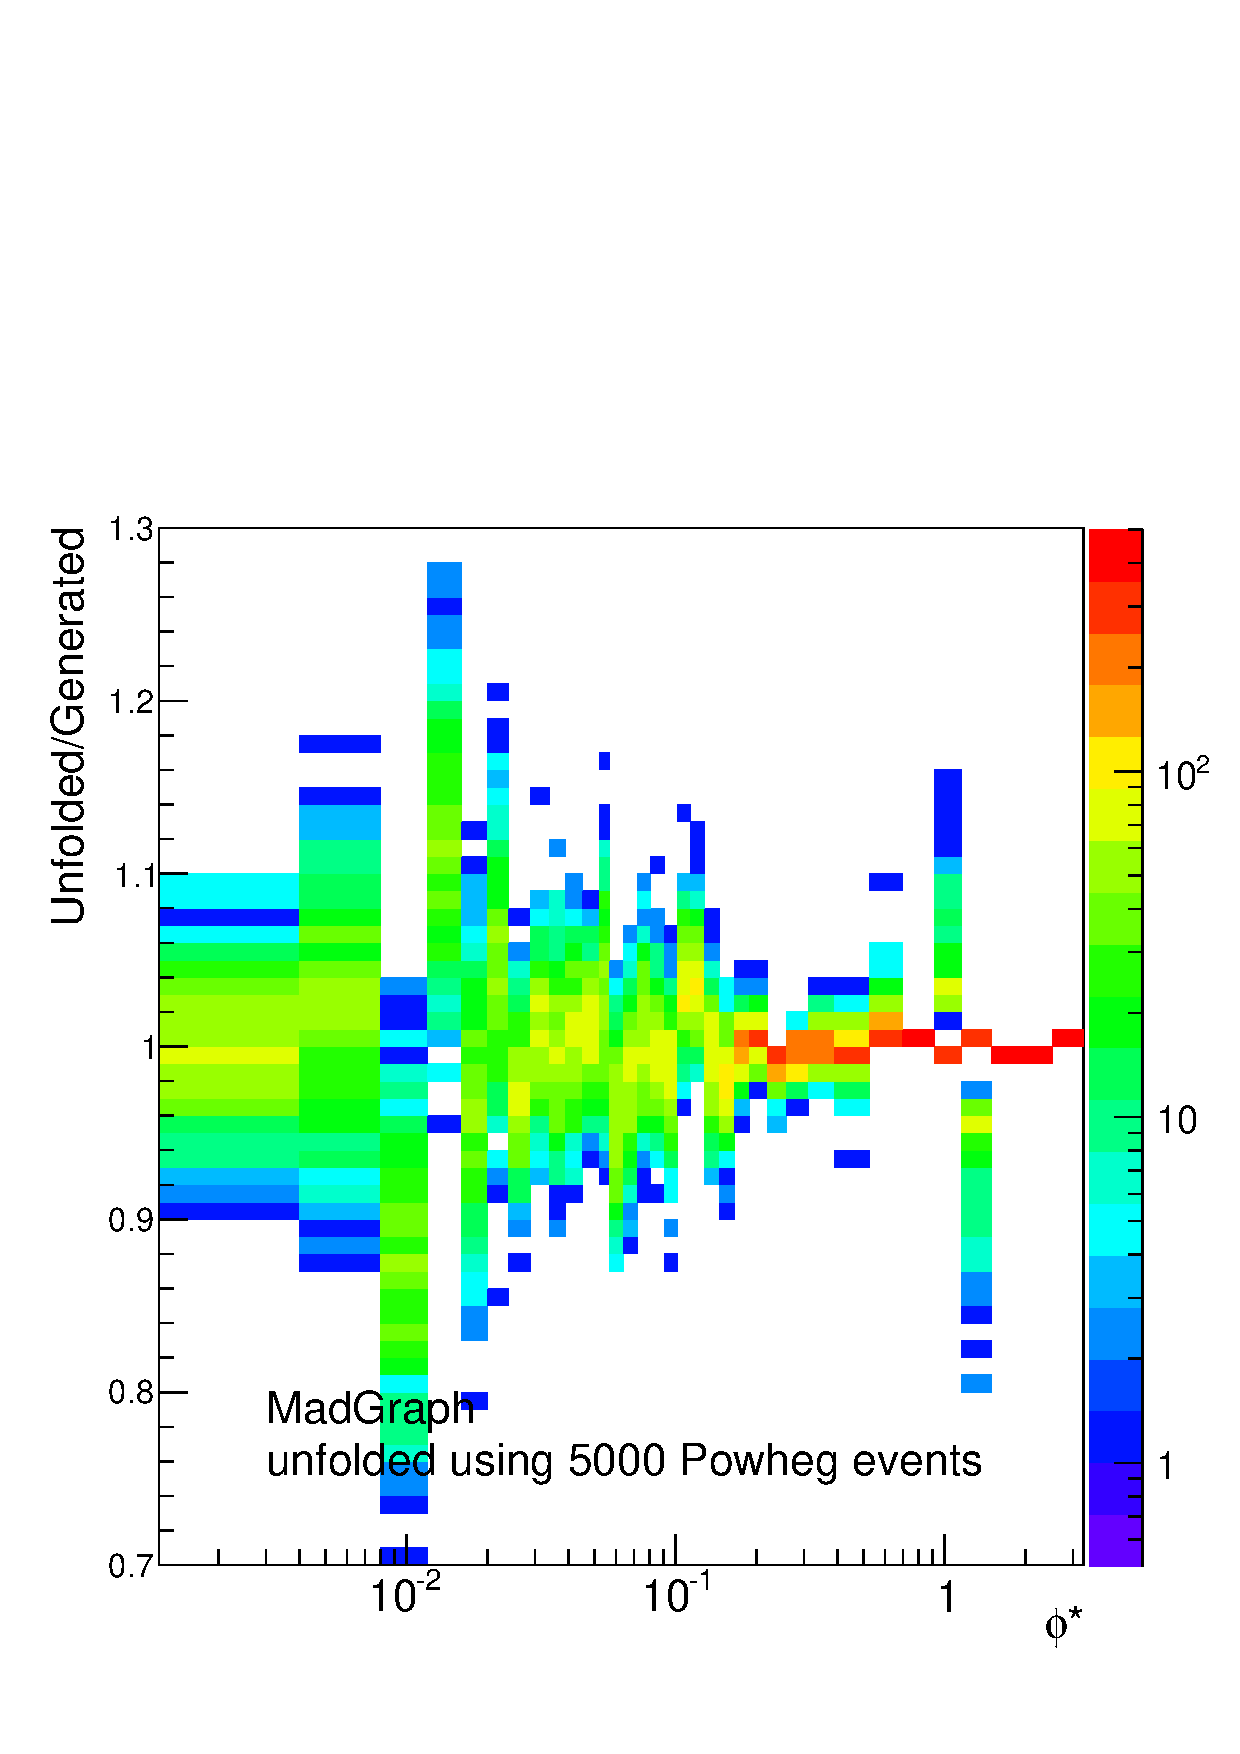
\includegraphics[width=\textwidth]{figures/ToyMC_PM_5000.pdf}
        \caption{}
        \label{fig:toy_mc_5000}
    \end{subfigure}% Make side by side
    \begin{subfigure}[b]{\SideBySidePlotWidth}
        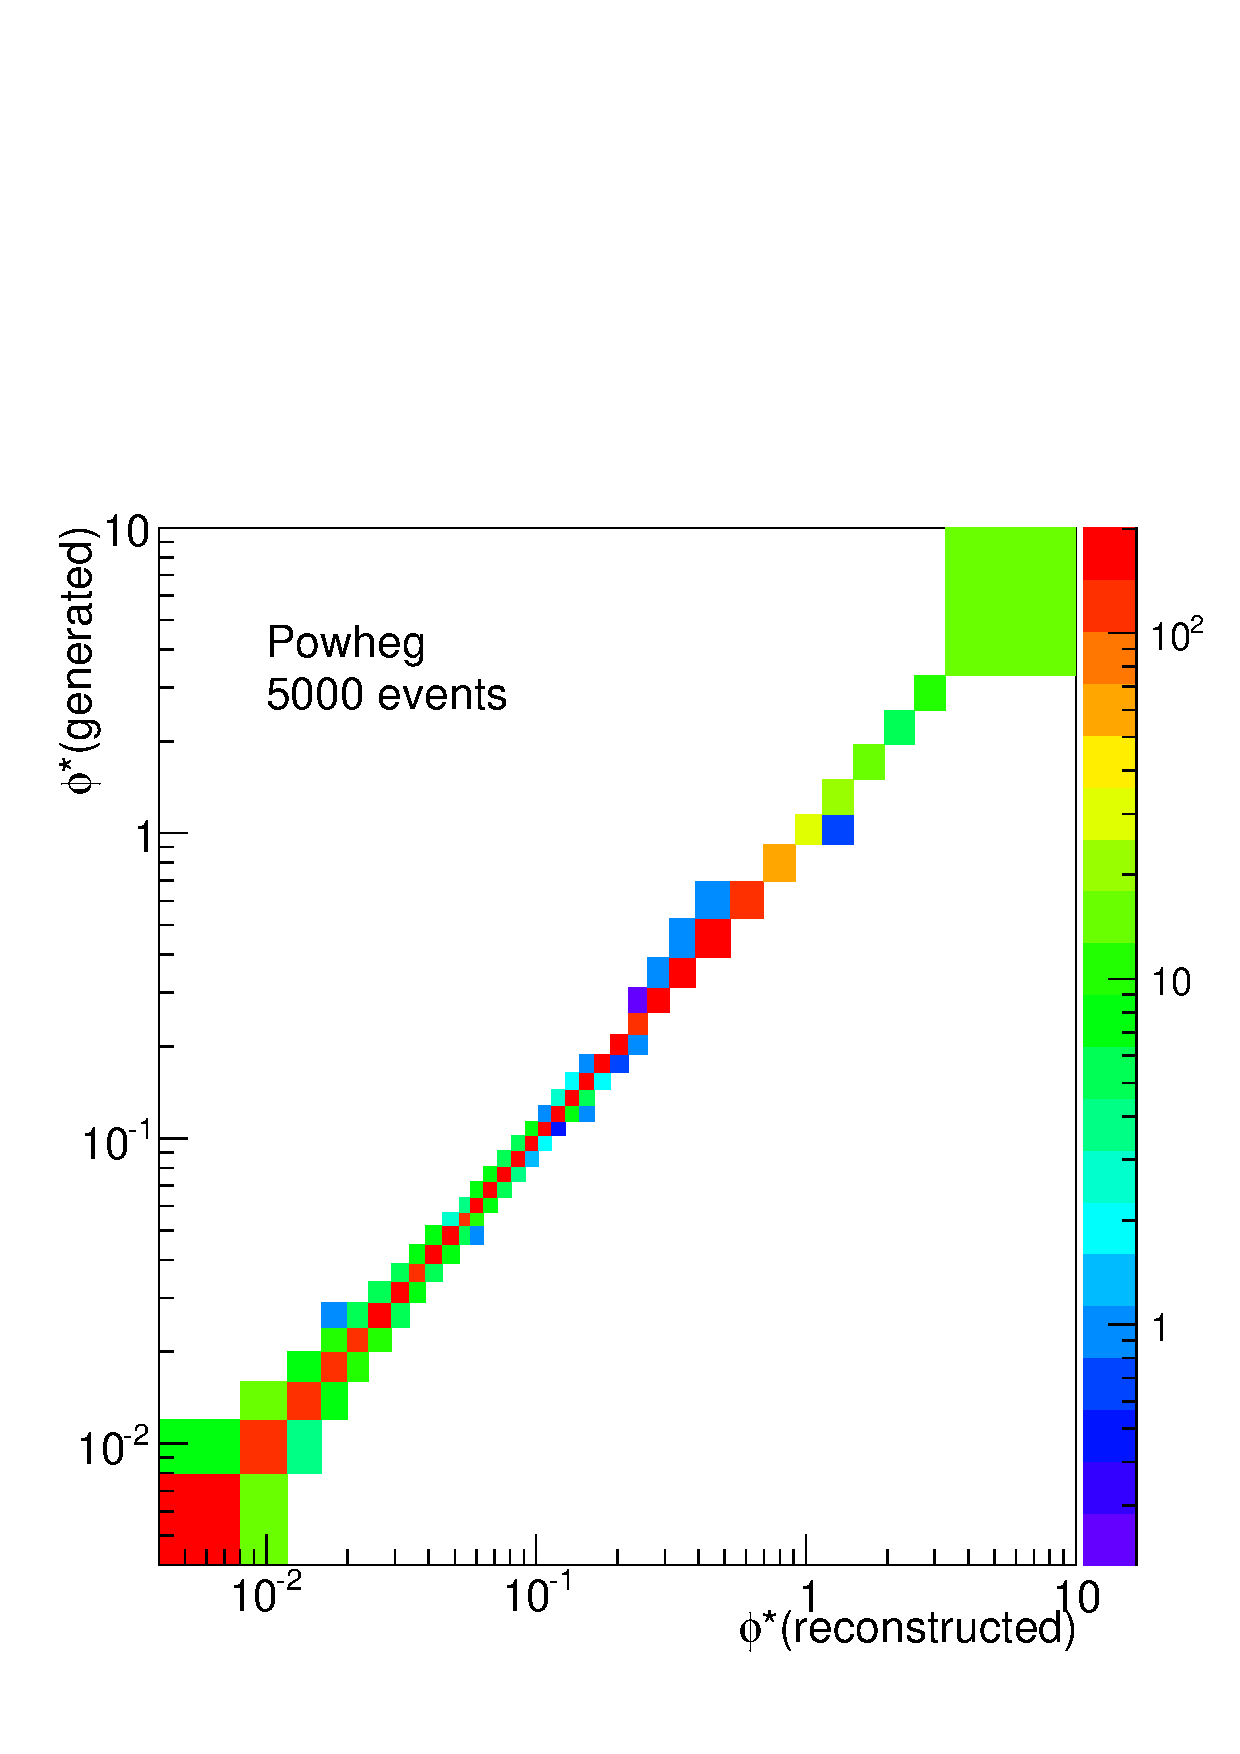
\includegraphics[width=\textwidth]{figures/BinM_P_5000.pdf}
        \caption{}
        \label{fig:bin_migration_5000}
    \end{subfigure}
    \caption{
        The ratio between the unfolded reconstructed \phistar distribution and
        the true generated \phistar distribution for \Ztoee events generated
        with \MADGRAPH is shown in (a). The unfolding was done with \num{5000}
        events from the \POWHEG sample. The distribution shown with circular
        points shows the results using the uncertainty propagation included in
        the \RooUnfold package. The distribution shown with square points is
        obtained by unfolding separately using 500 toy MC variations of the bin
        migration matrix. The pull of the bins in (a) are shown in (b). All
        \num{500} unfolded toy MC variations and the initial nominal
        distribution used to produce (a) are shown in (c). The bin migration
        matrix based on \num{5000} events from the \POWHEG sample, used to
        produce (a) is shown in (d).
    }
\label{fig:5000_propegation_unfolding}
\end{figure}

At large \phistar values the uncertainty calculated with the toy MC method goes
to \num{0}. This is because there are no off-diagonal bins in this region of
the original bin migration matrix and so no off-diagonal bins are allowed to
appear due to our fluctuations. This problem is greatly reduced as we use more
generator level events to construct the matrix, as can be seen in
\FIGS~\ref{fig:50000_propegation_unfolding} and
\ref{fig:full_propegation_unfolding}.

\begin{figure}[!htbp]
    \centering
    \begin{subfigure}[b]{\SideBySidePlotWidth}
        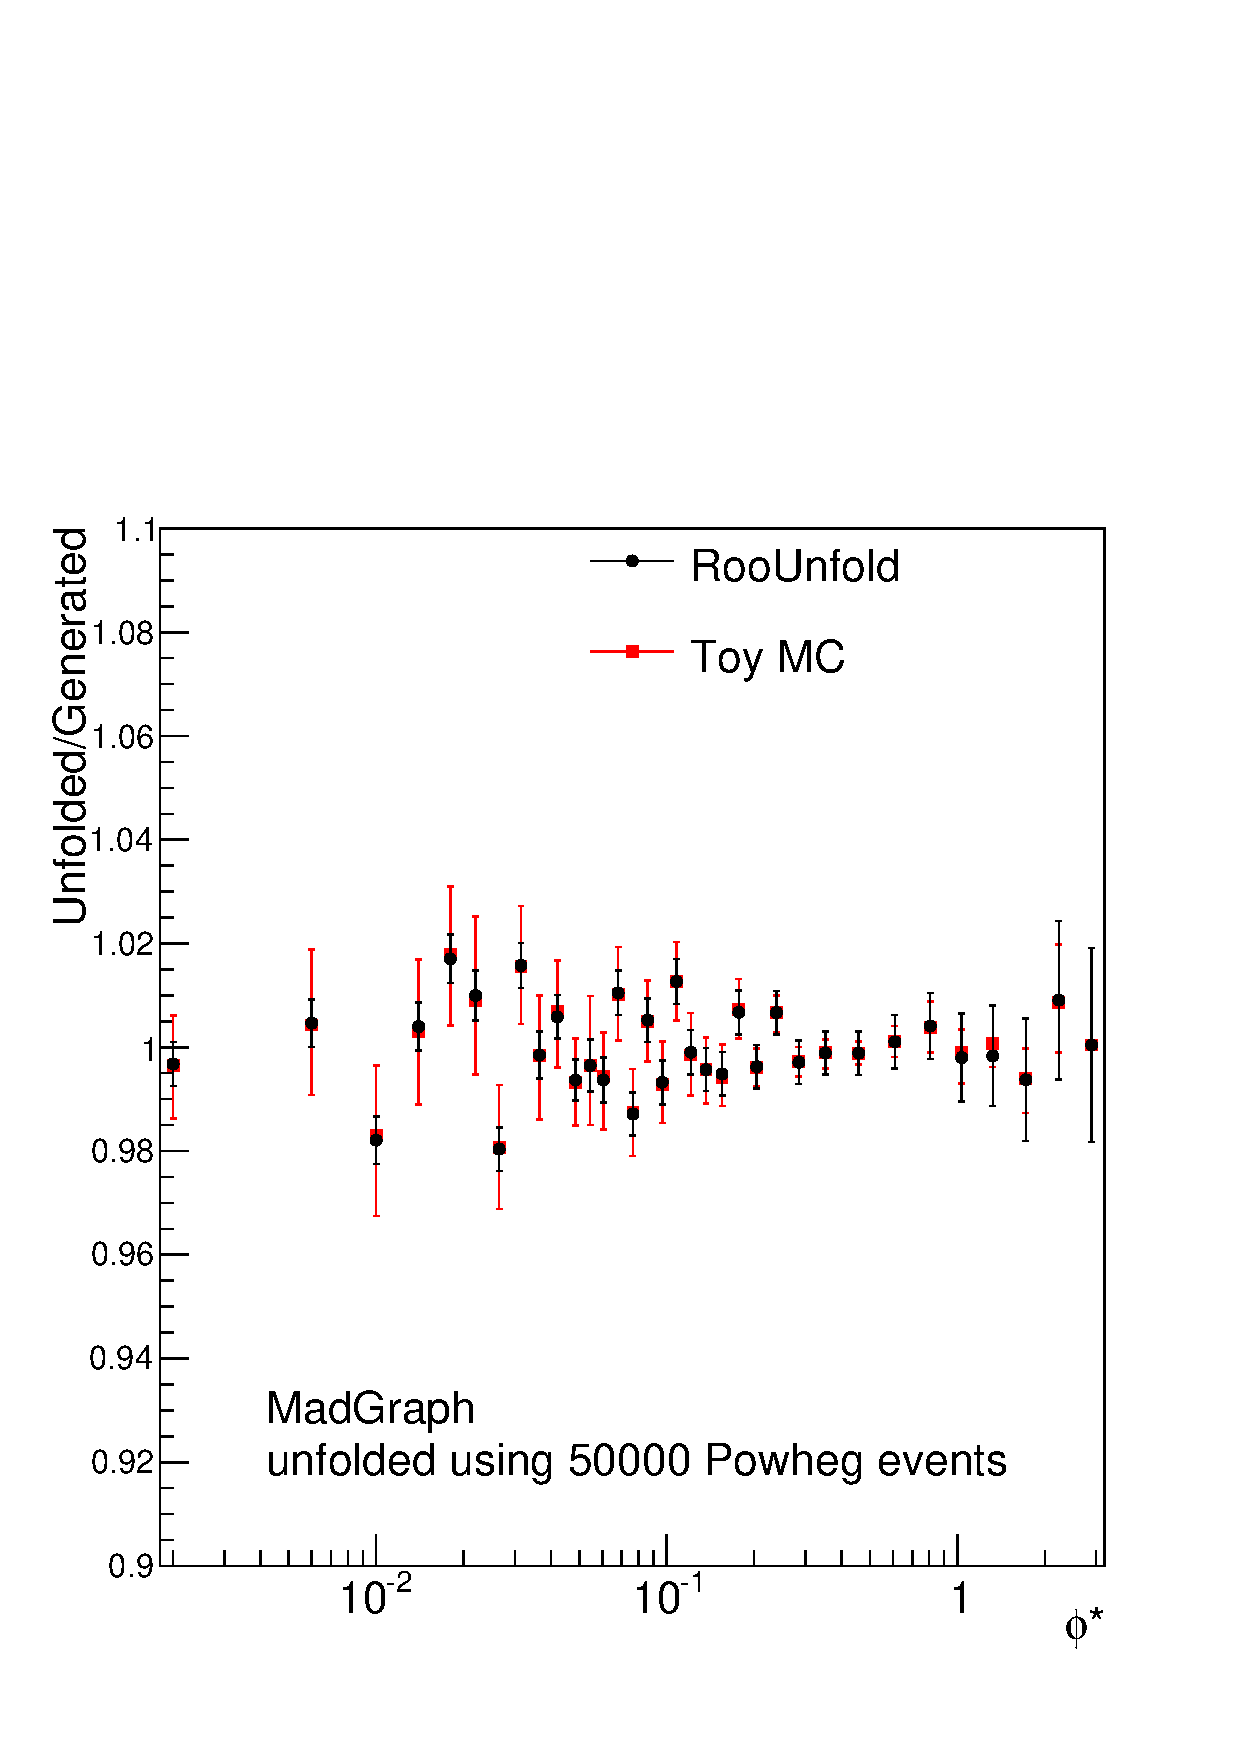
\includegraphics[width=\textwidth]{figures/BinM_PM_50000.pdf}
        \caption{}
        \label{fig:unfolding_madgraph_with_50000}
    \end{subfigure}% Make side by side
    \begin{subfigure}[b]{\SideBySidePlotWidth}
        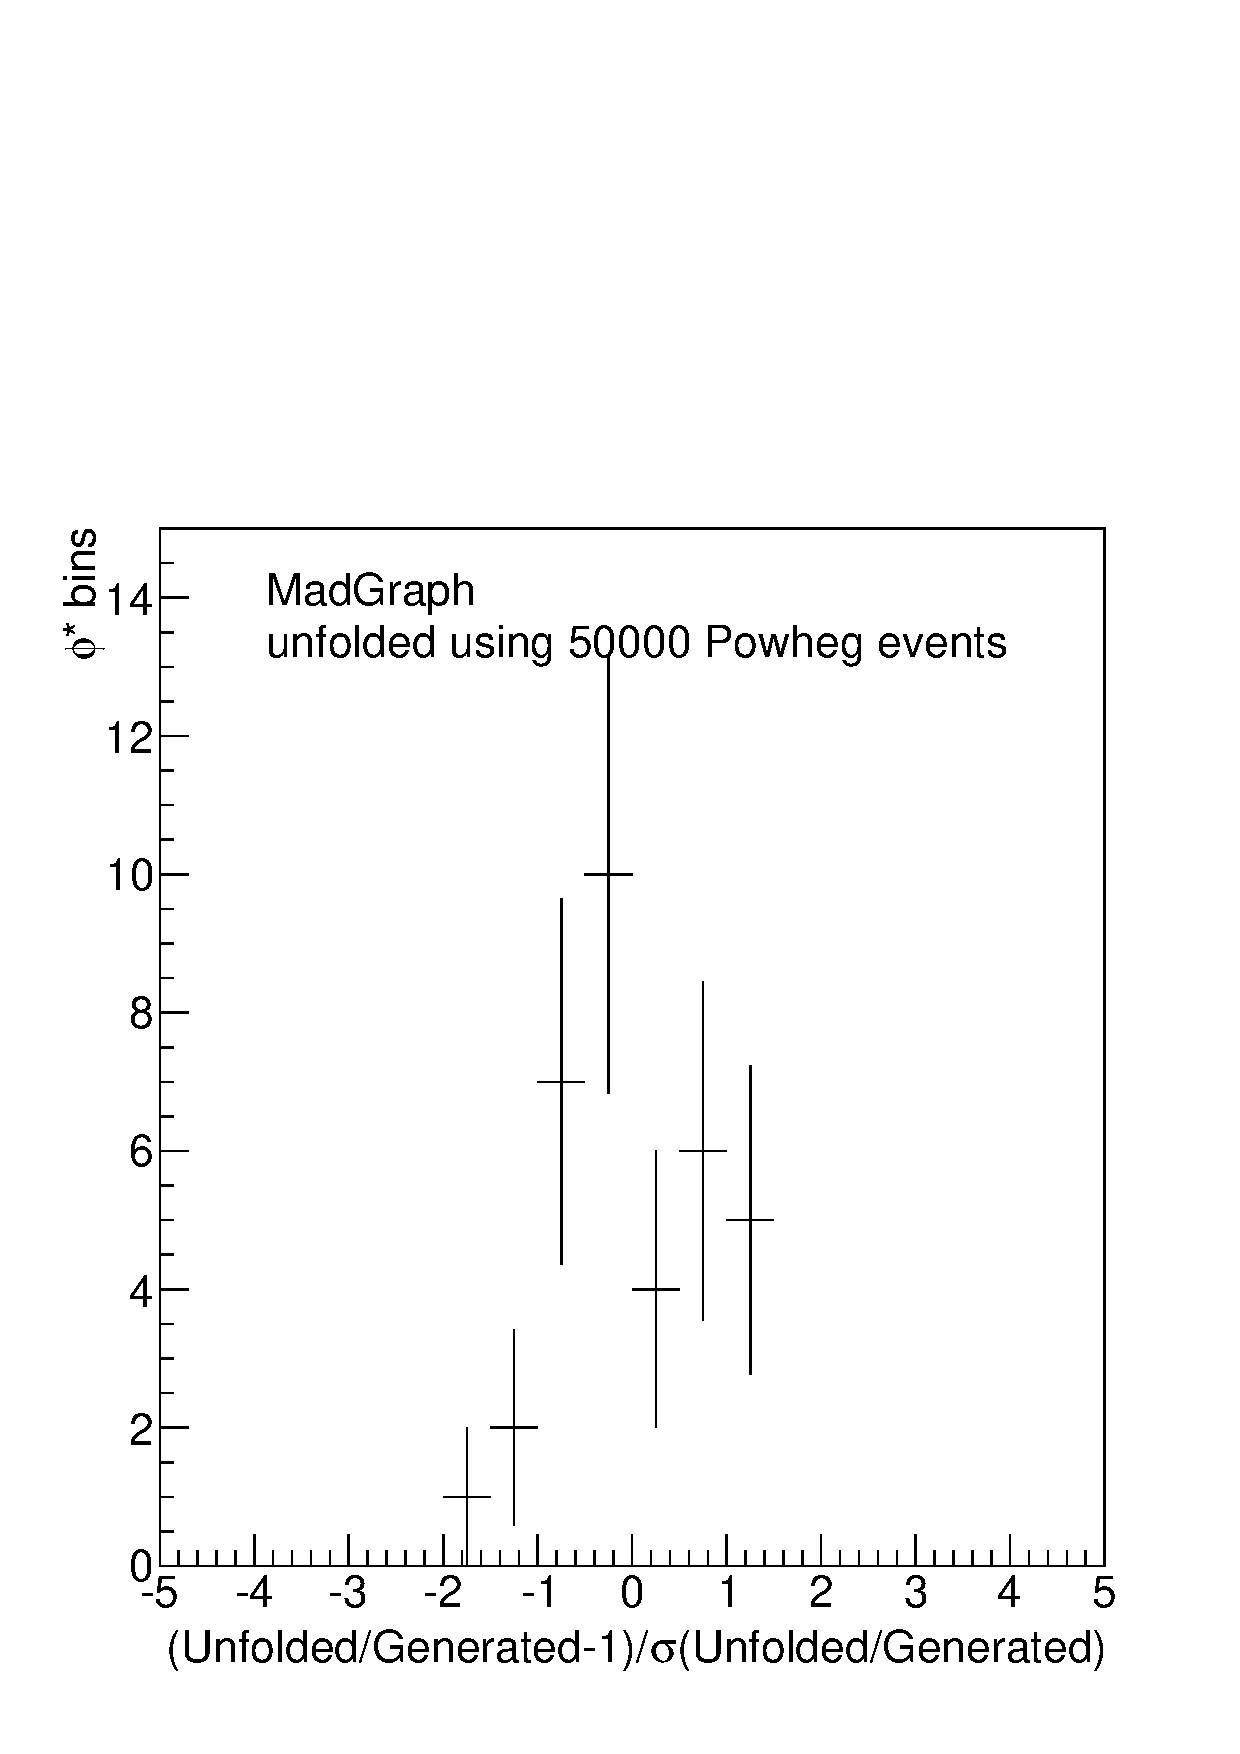
\includegraphics[width=\textwidth]{figures/Pull_50000.pdf}
        \caption{}
        \label{fig:pull_50000}
    \end{subfigure}
    \begin{subfigure}[b]{\SideBySidePlotWidth}
        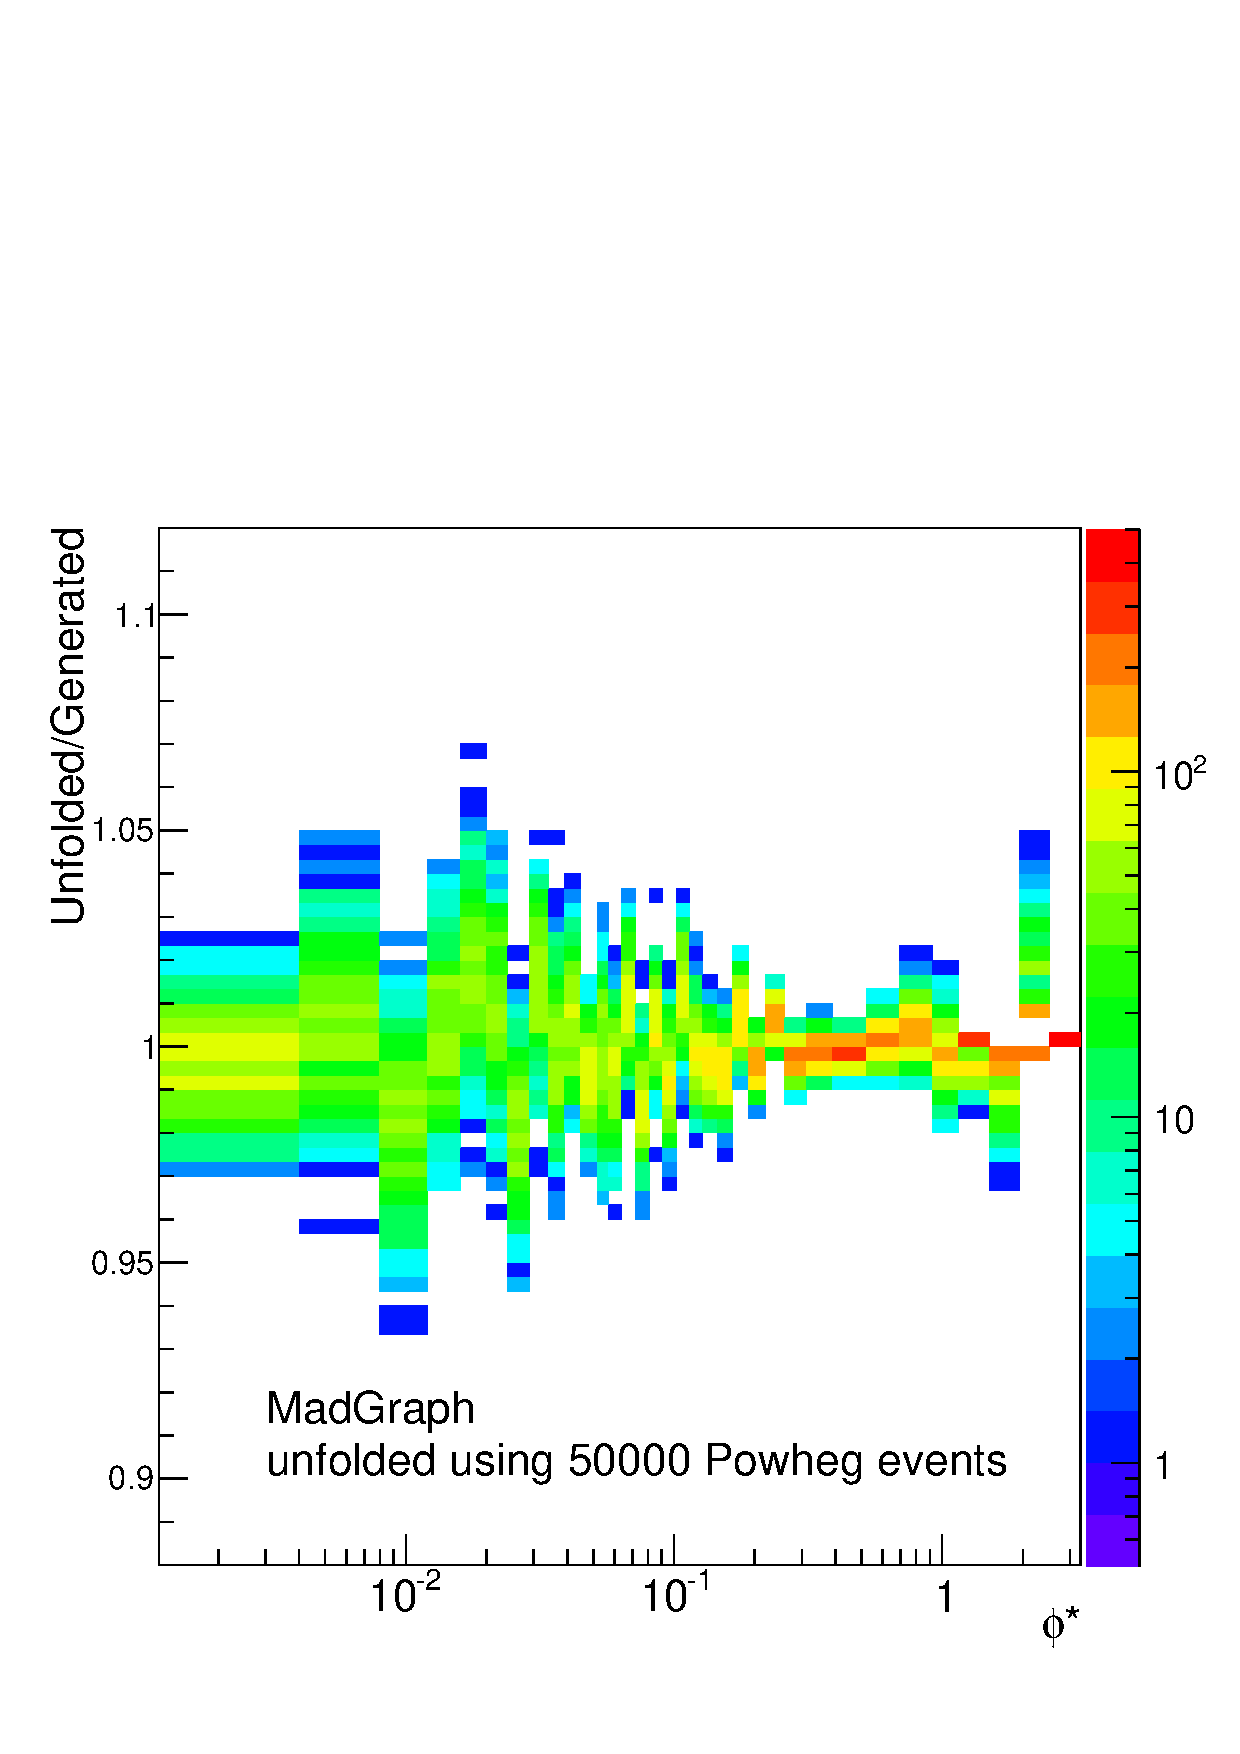
\includegraphics[width=\textwidth]{figures/ToyMC_PM_50000.pdf}
        \caption{}
        \label{fig:toy_mc_50000}
    \end{subfigure}% Make side by side
    \begin{subfigure}[b]{\SideBySidePlotWidth}
        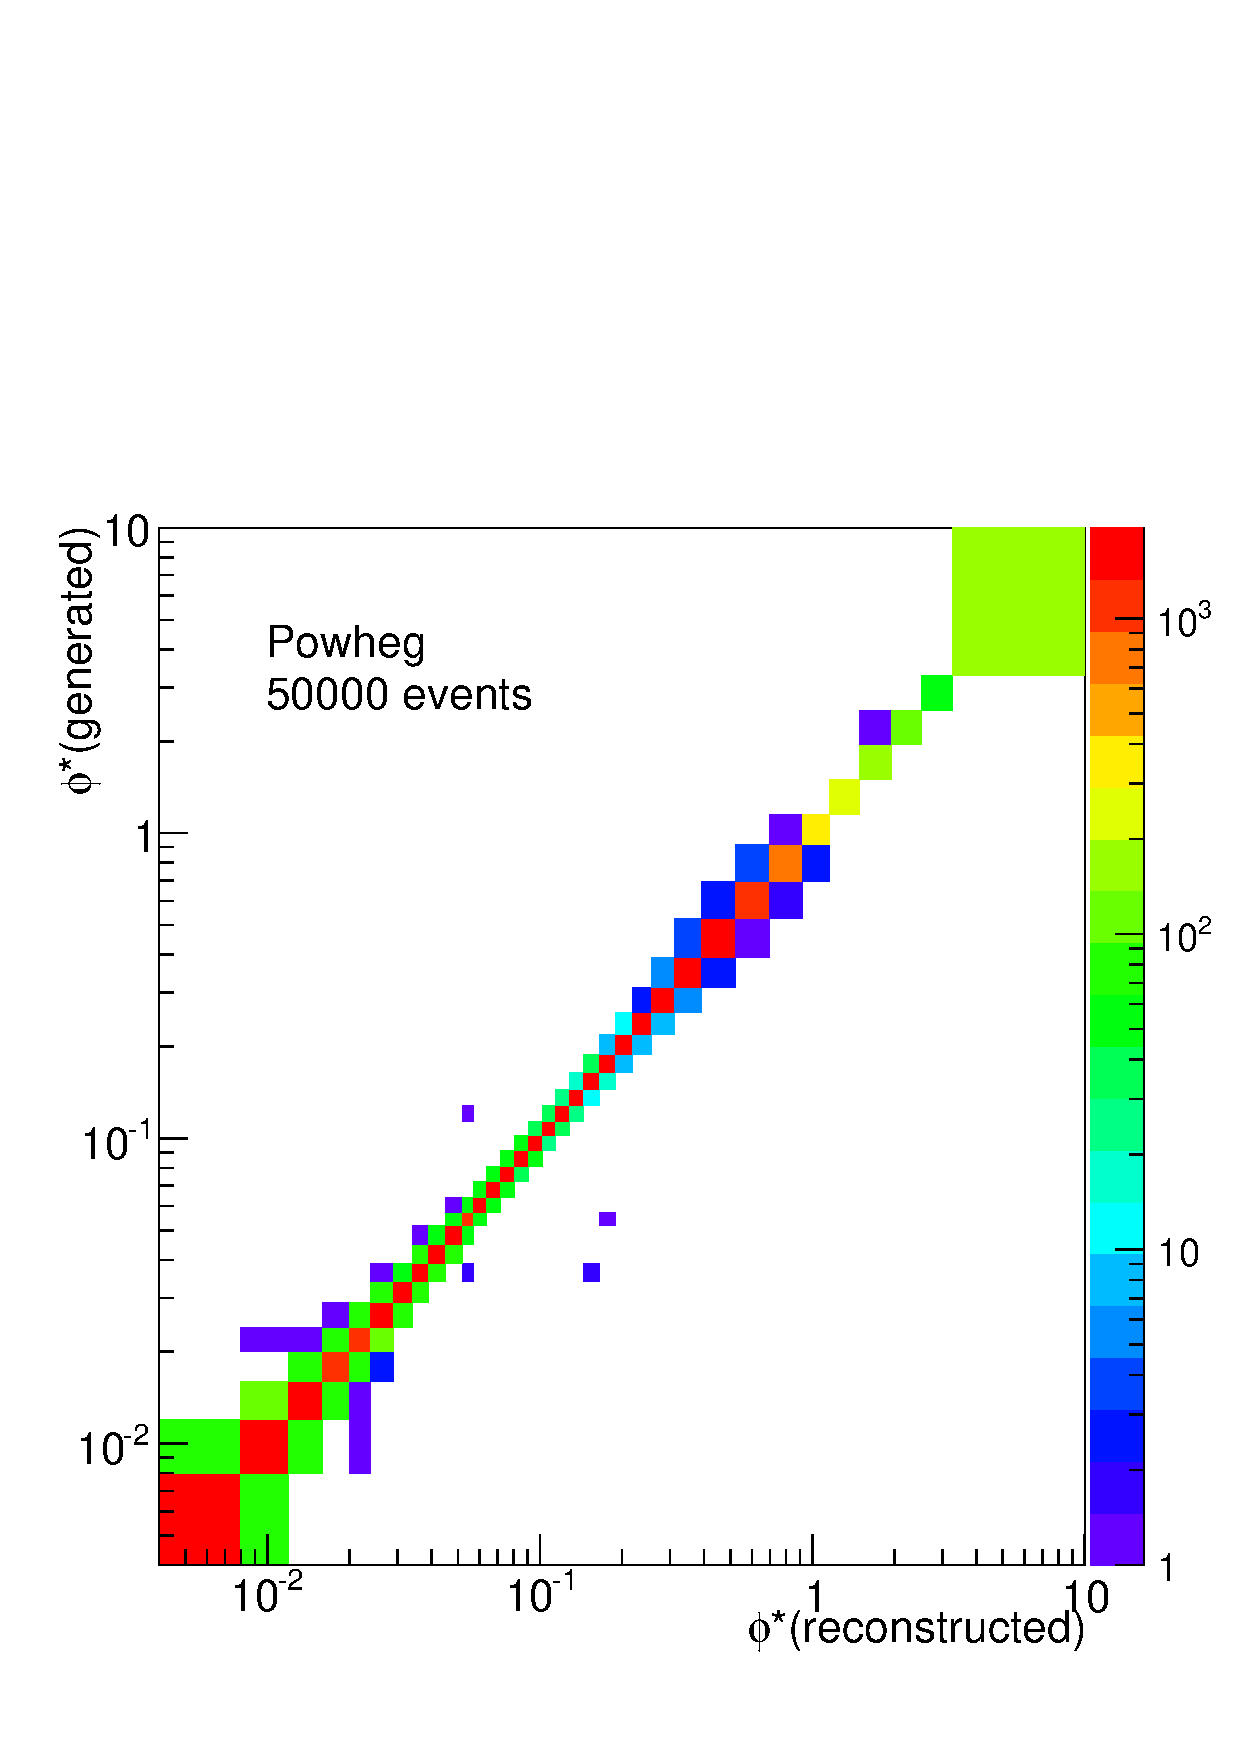
\includegraphics[width=\textwidth]{figures/BinM_P_50000.pdf}
        \caption{}
        \label{fig:bin_migration_50000}
    \end{subfigure}
    \caption{
        The ratio between the unfolded reconstructed \phistar distribution and
        the true generated \phistar distribution for \Ztoee events generated
        with \MADGRAPH is shown in (a). The unfolding was done with \num{50000}
        events from the \POWHEG sample. The distribution shown with circular
        points shows the results using the uncertainty propagation included in
        the \RooUnfold package. The distribution shown with square points is
        obtained by unfolding separately using 500 toy MC variations of the bin
        migration matrix. The pull of the bins in (a) are shown in (b). All
        \num{500} unfolded toy MC variations and the initial nominal
        distribution used to produce (a) are shown in (c). The bin migration
        matrix based on \num{50000} events from the \POWHEG sample, used to
        produce (a) is shown in (d).
    }
\label{fig:50000_propegation_unfolding}
\end{figure}

\begin{figure}[!htbp]
    \centering
    \begin{subfigure}[b]{\SideBySidePlotWidth}
        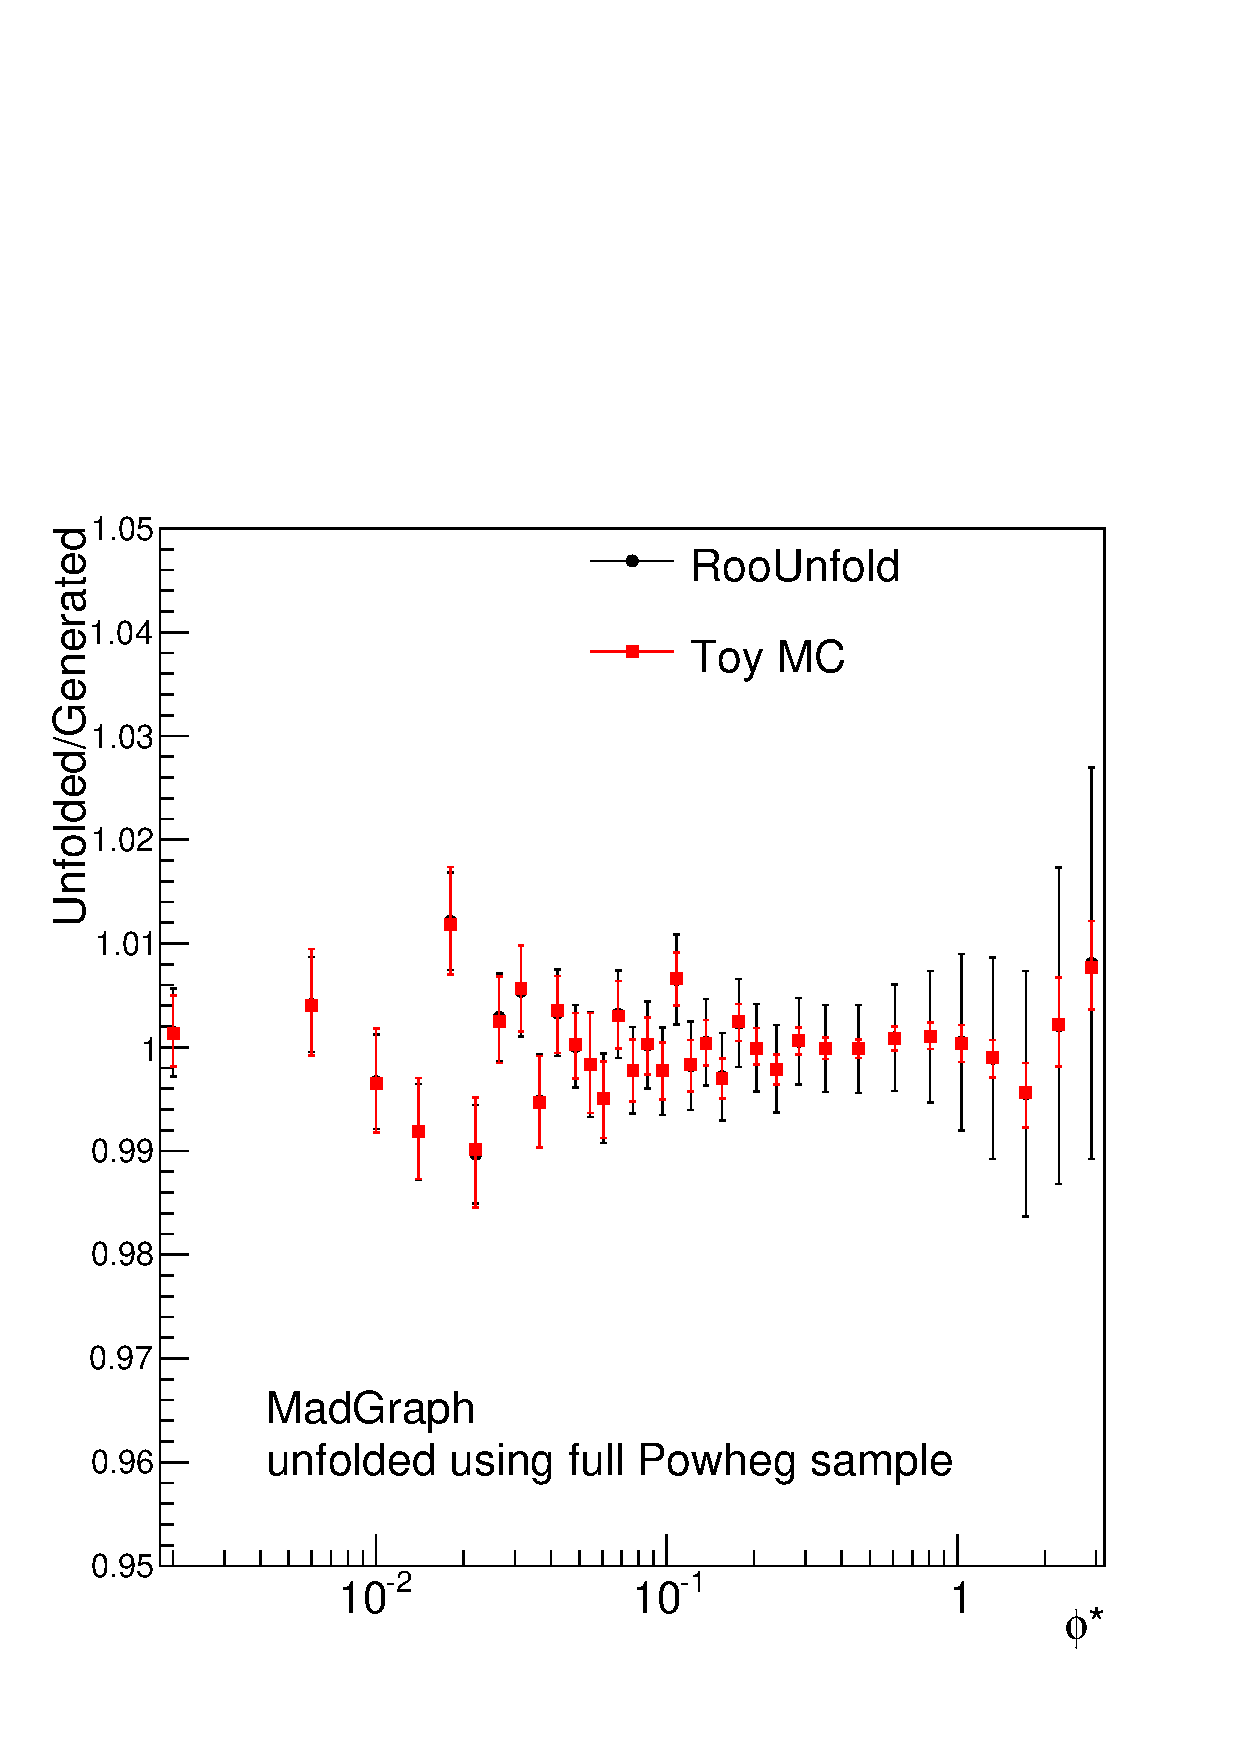
\includegraphics[width=\textwidth]{figures/BinM_PM_ALL.pdf}
        \caption{}
        \label{fig:unfolding_madgraph_with_all}
    \end{subfigure}% Make side by side
    \begin{subfigure}[b]{\SideBySidePlotWidth}
        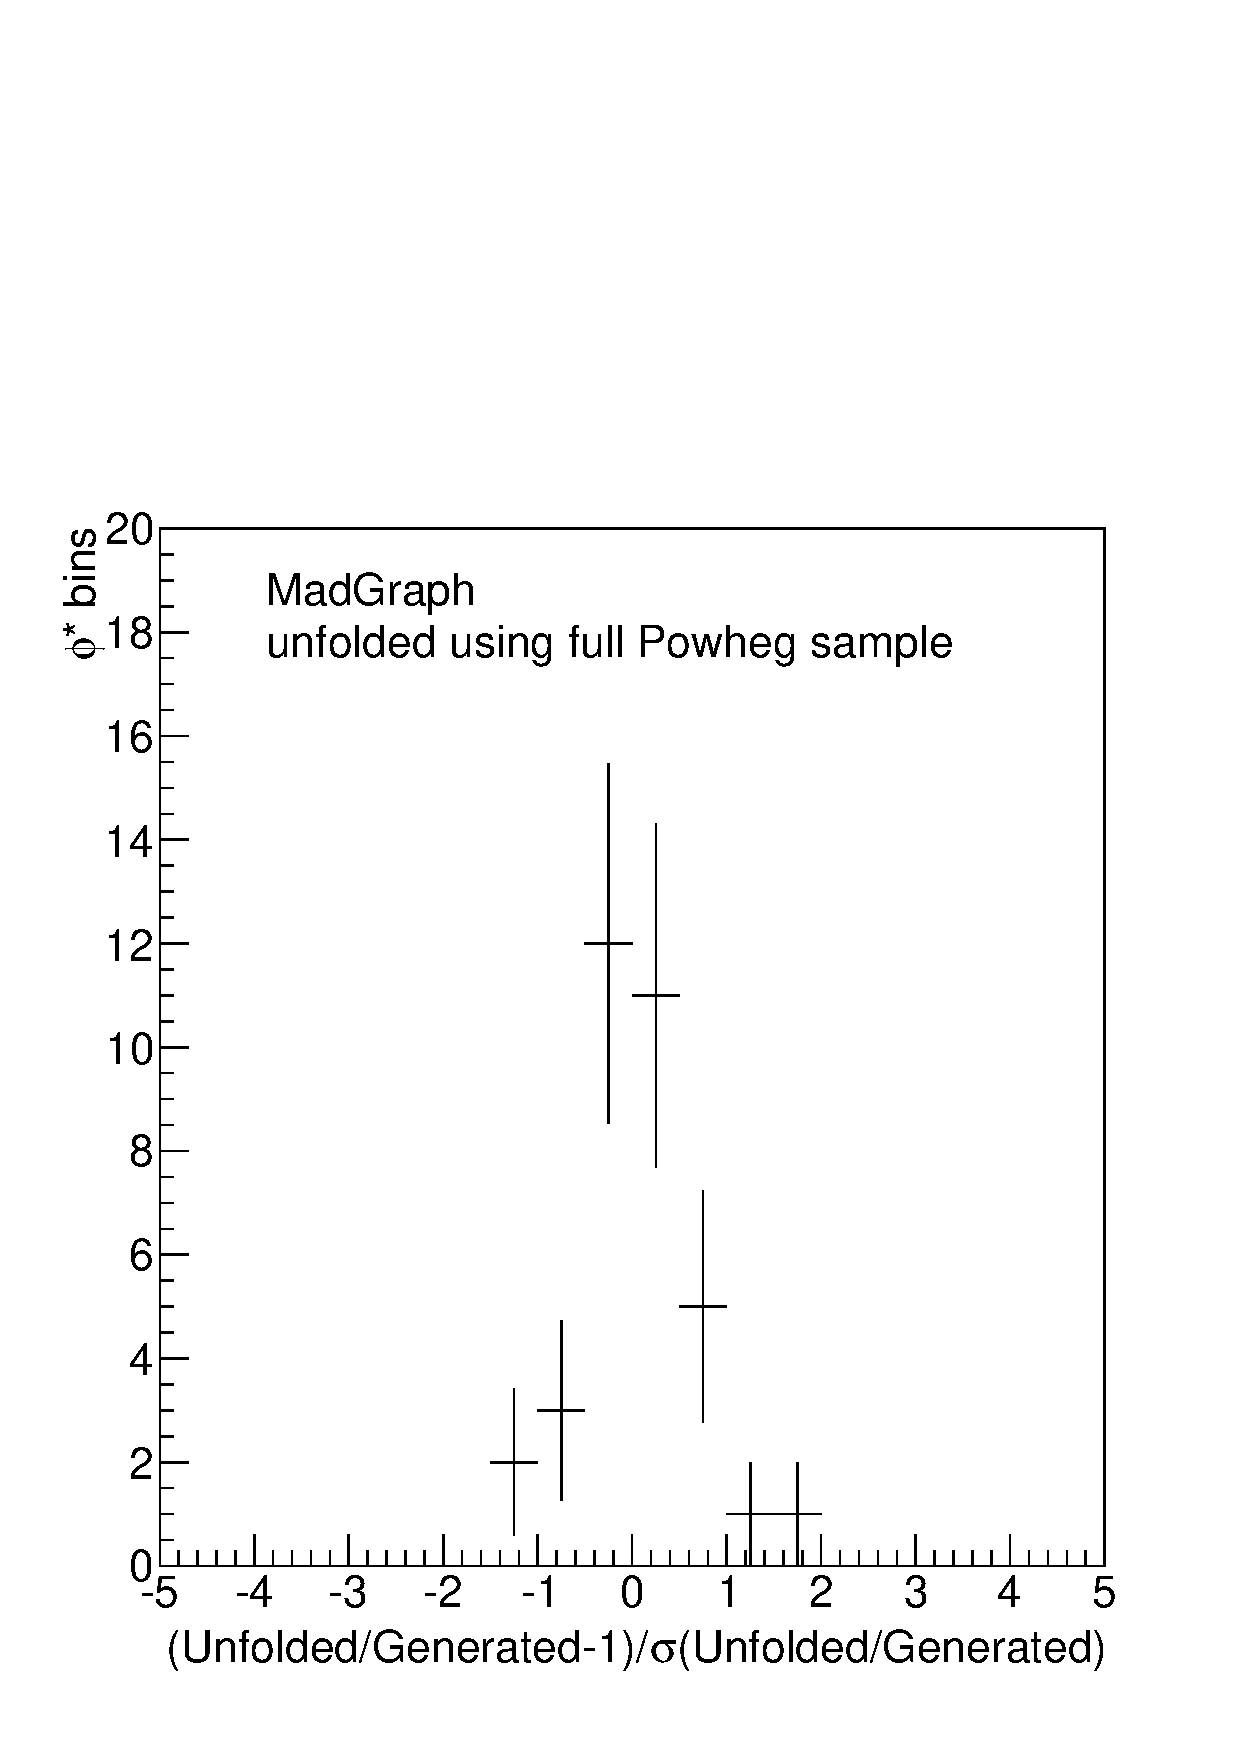
\includegraphics[width=\textwidth]{figures/Pull_ALL.pdf}
        \caption{}
        \label{fig:pull_all}
    \end{subfigure}
    \begin{subfigure}[b]{\SideBySidePlotWidth}
        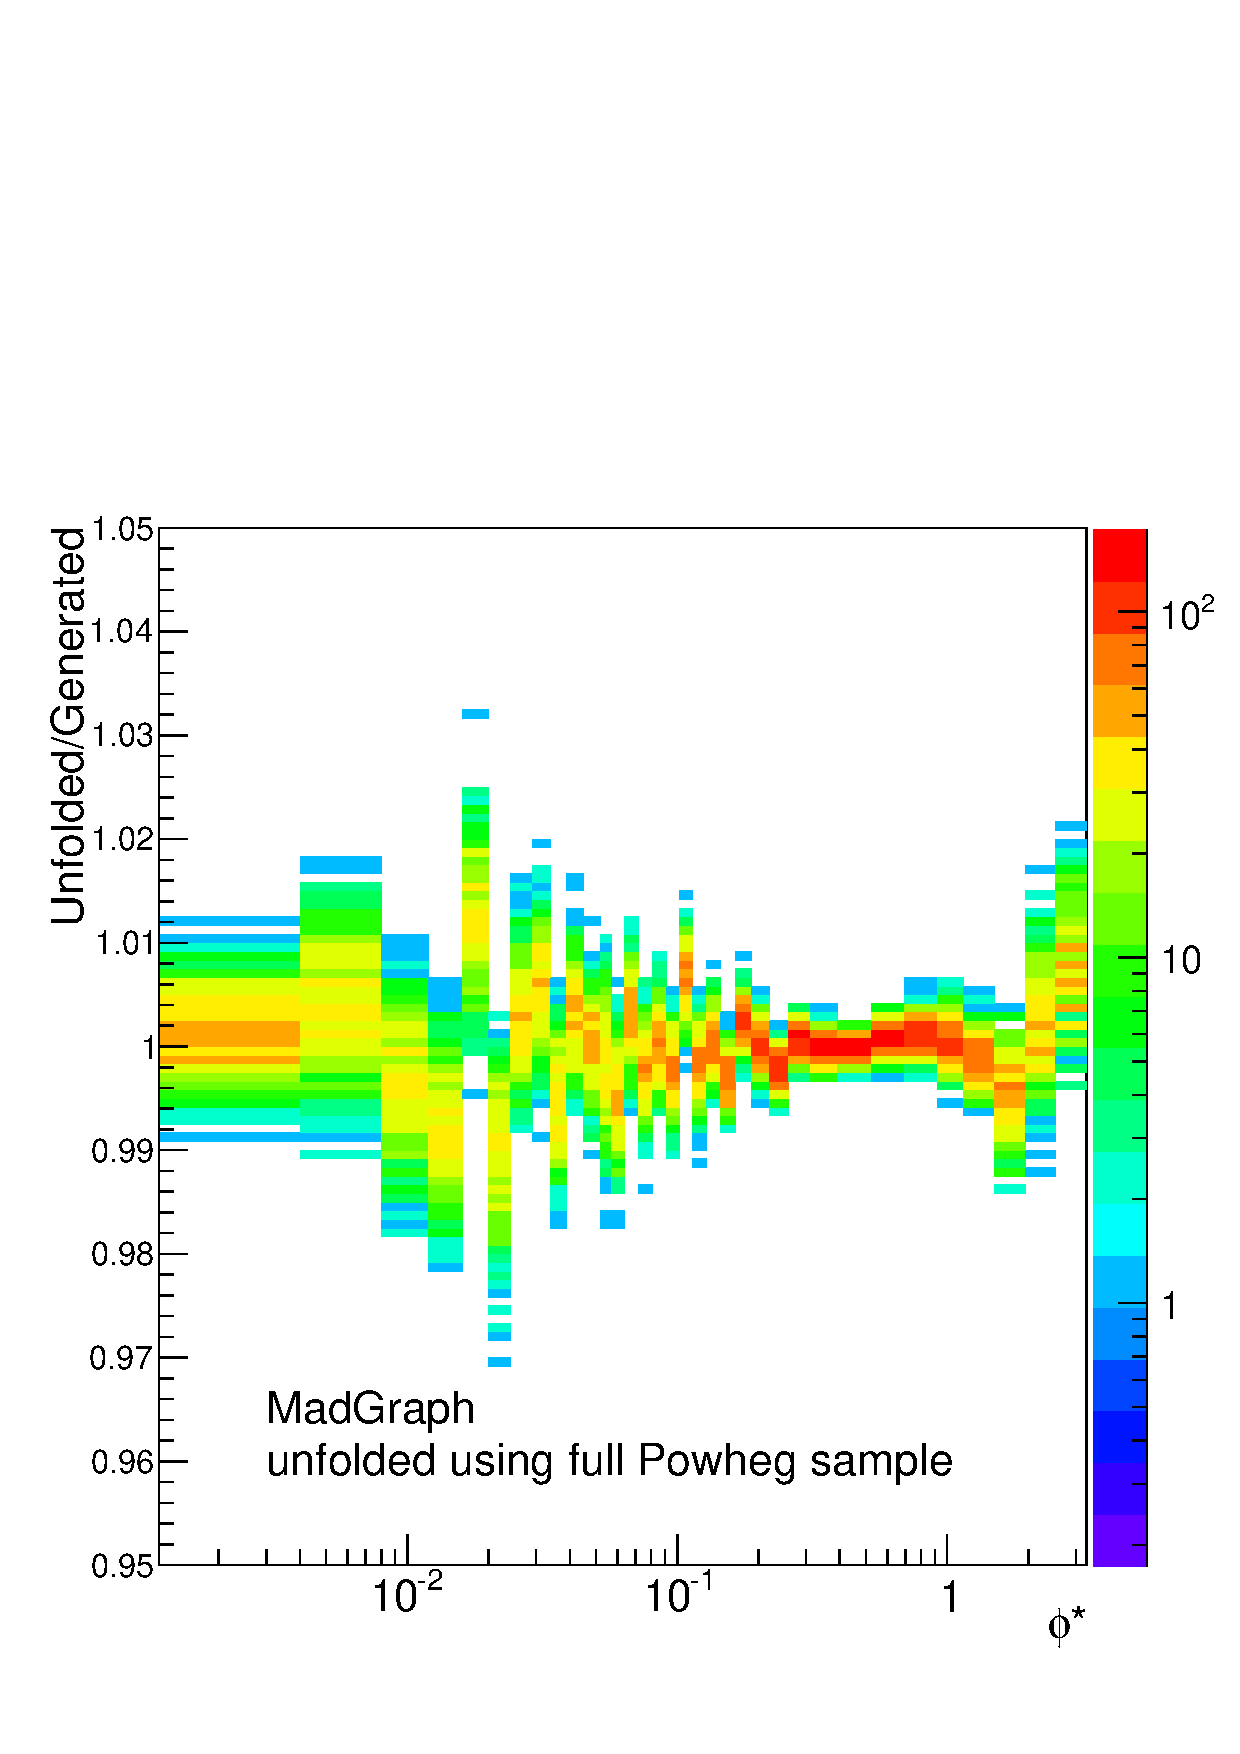
\includegraphics[width=\textwidth]{figures/ToyMC_PM_ALL.pdf}
        \caption{}
        \label{fig:toy_mc_all}
    \end{subfigure}% Make side by side
    \begin{subfigure}[b]{\SideBySidePlotWidth}
        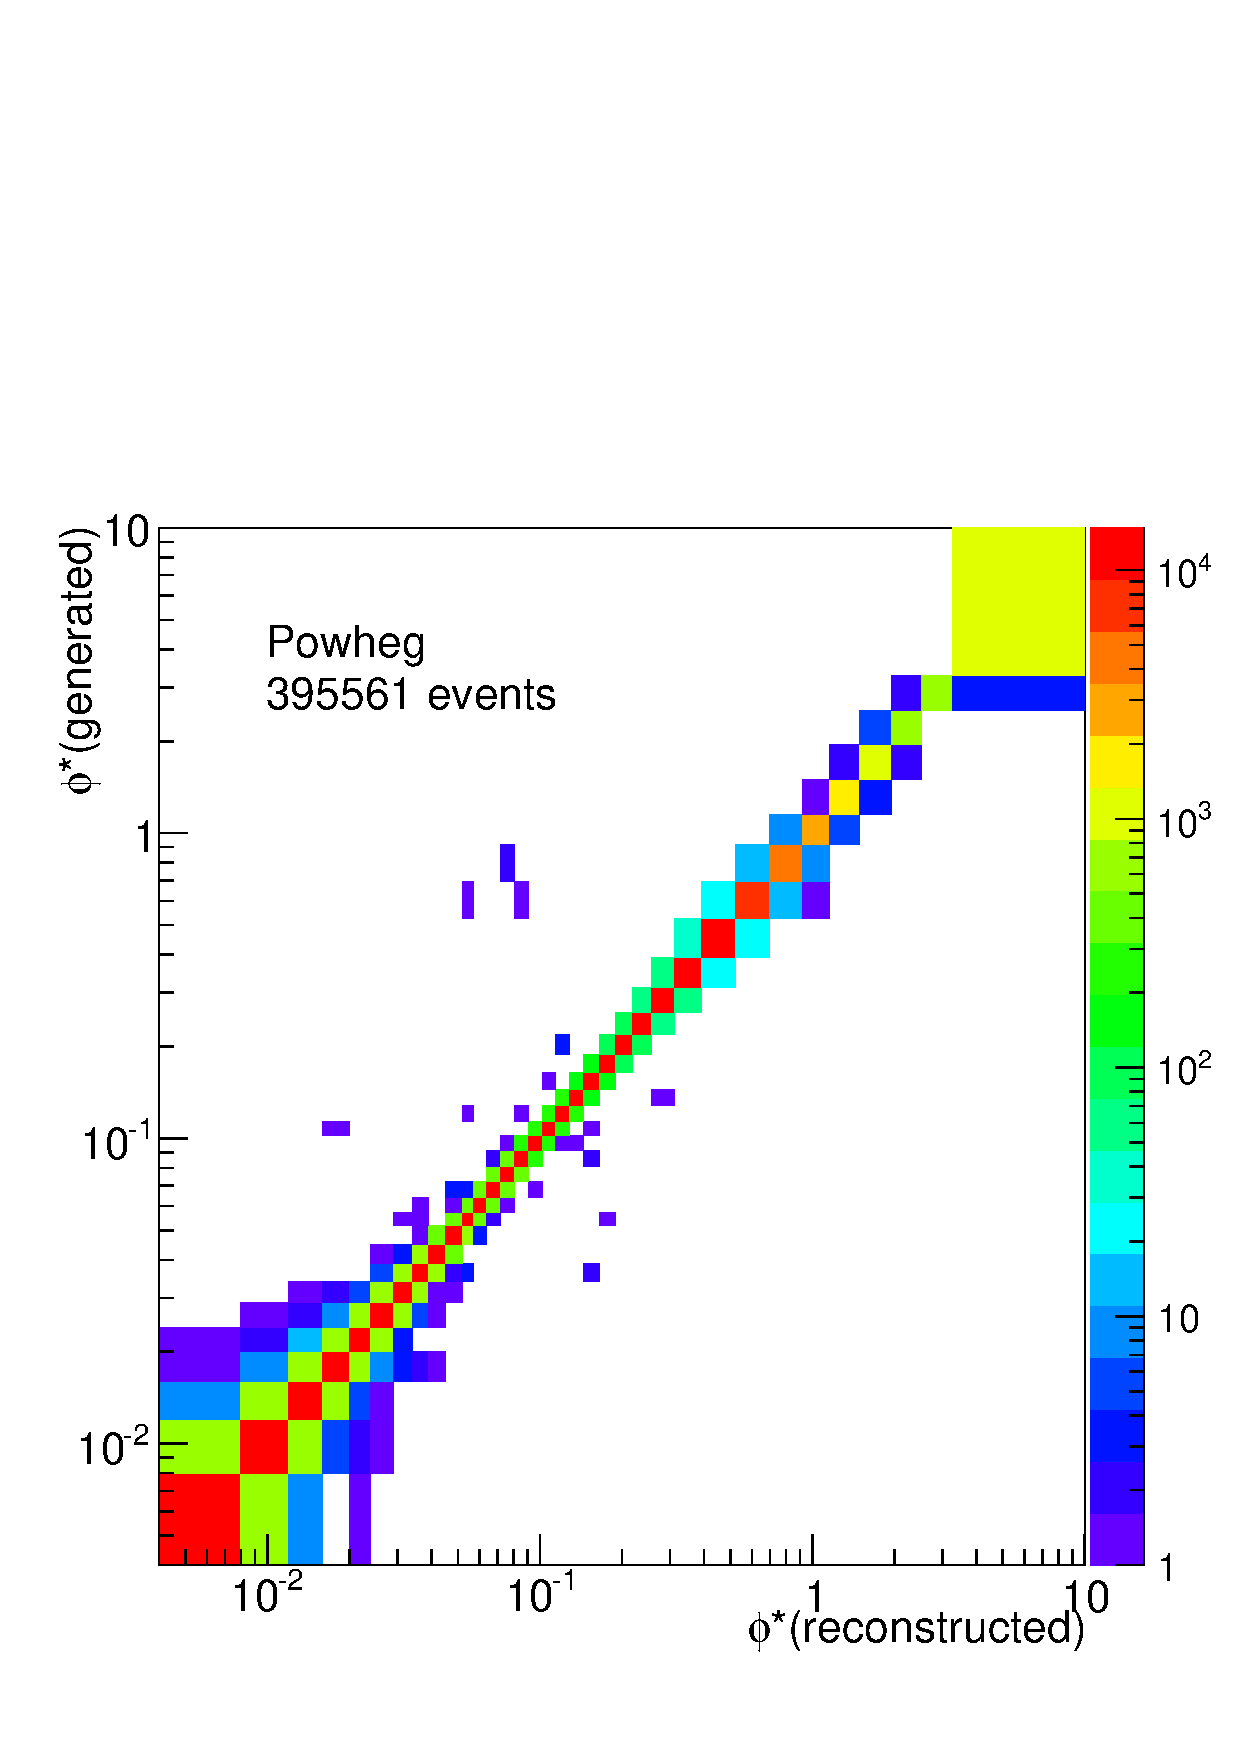
\includegraphics[width=\textwidth]{figures/BinM_P_ALL.pdf}
        \caption{}
        \label{fig:bin_migration_all}
    \end{subfigure}
    \caption{
        The ratio between the unfolded reconstructed \phistar distribution and
        the true generated \phistar distribution for \Ztoee events generated
        with \MADGRAPH is shown in (a). The unfolding was done with all events
        from the \POWHEG sample. The distribution shown with circular points
        shows the results using the uncertainty propagation included in the
        \RooUnfold package. The distribution shown with square points is
        obtained by unfolding separately using 500 toy MC variations of the bin
        migration matrix. The pull of the bins in (a) are shown in (b). All
        \num{500} unfolded toy MC variations and the initial nominal
        distribution used to produce (a) are shown in (c). The bin migration
        matrix based on all events from the \POWHEG sample, used to produce (a)
        is shown in (d).
    }
\label{fig:full_propegation_unfolding}
\end{figure}

The total statistical uncertainty due to the bin migration unfolding is the
sum of the uncertainty reported by \RooUnfold due to the number of events in
the data and the uncertainty calculated using the toy MC method in quadrature.

\subsubsection{Systematic Uncertainties}
\label{ssec:unfolding_systematic_uncertainties}

The unfolding to correct for bin migration is dependent on the way in which the
bin migration is simulated in MC. Differences in the \phistar distribution
between MC and data can lead to systematic uncertainties on the final result.
Two such potential differences between the MC and the data are considered. The
first potential difference is in the shape of the \phistar distribution, and
the second is in the resolution of the \phistar distribution.

One of the advantages of the Bayesian unfolding method used in this analysis is
that it, unlike a simpler bin-by-bin correction, is theoretically insensitive
to the distribution of \phistar at the generator level. In fact, \DAgostini
recommends using a flat generated distribution as one easy method of ensuring
that there are enough generated events in each bin \cite{dagostini_1995}.
\TODO{Cite twice in same chapter?} We use this recommendation as the basis for
a test of the systematic uncertainty. The \phistar distribution at the
generator level in the \MADGRAPH sample is inserted into a histogram with bin
widths of $\phistar = 0.011$. Each bin is weighted with a weight equal to the
inverse number of events in the bin so that the distribution is flattened. The
full \POWHEG sample is then unfolded using this \MADGRAPH distribution. The
response matrix from this modified \MADGRAPH distribution is show in
\FIG~\ref{fig:unfolding_flat_bin_migration}. The ratio of the unfolded \POWHEG
distribution over the generated distribution is shown in
\FIG~\ref{fig:unfolding_flat_powheg_unfolded_with_madgraph}. This ratio uses
only the uncertainties provided by \RooUnfold and so underestimates the total
uncertainty. No deviations from \num{1} are seen, and so no systematic
uncertainty is assigned for the shape of the generator level \phistar
distribution.

\begin{figure}[!htbp]
    \centering
    \begin{subfigure}[b]{\SideBySidePlotWidth}
        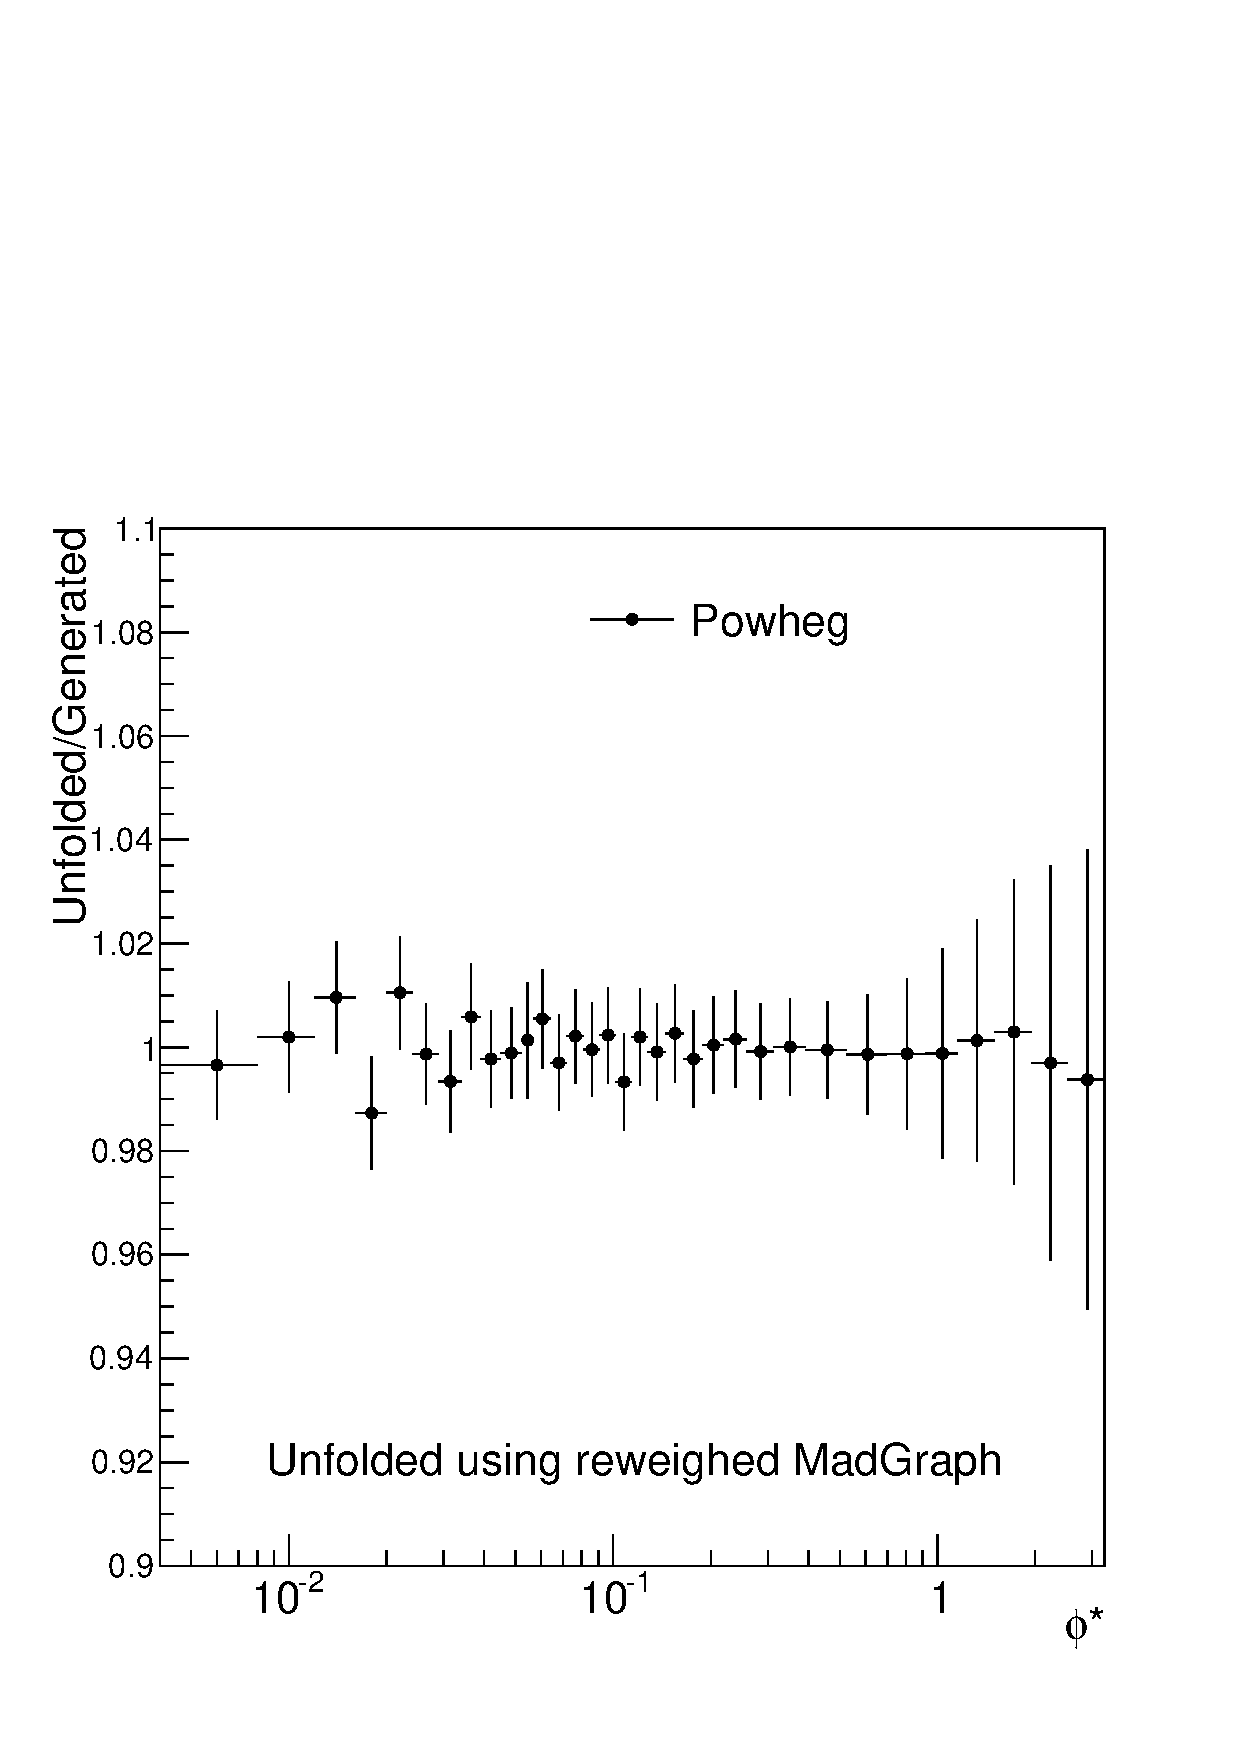
\includegraphics[width=\textwidth]{figures/BinM_MP_flat.pdf}
        \caption{}
        \label{fig:unfolding_flat_powheg_unfolded_with_madgraph}
    \end{subfigure}% Make side by side
    \begin{subfigure}[b]{\SideBySidePlotWidth}
        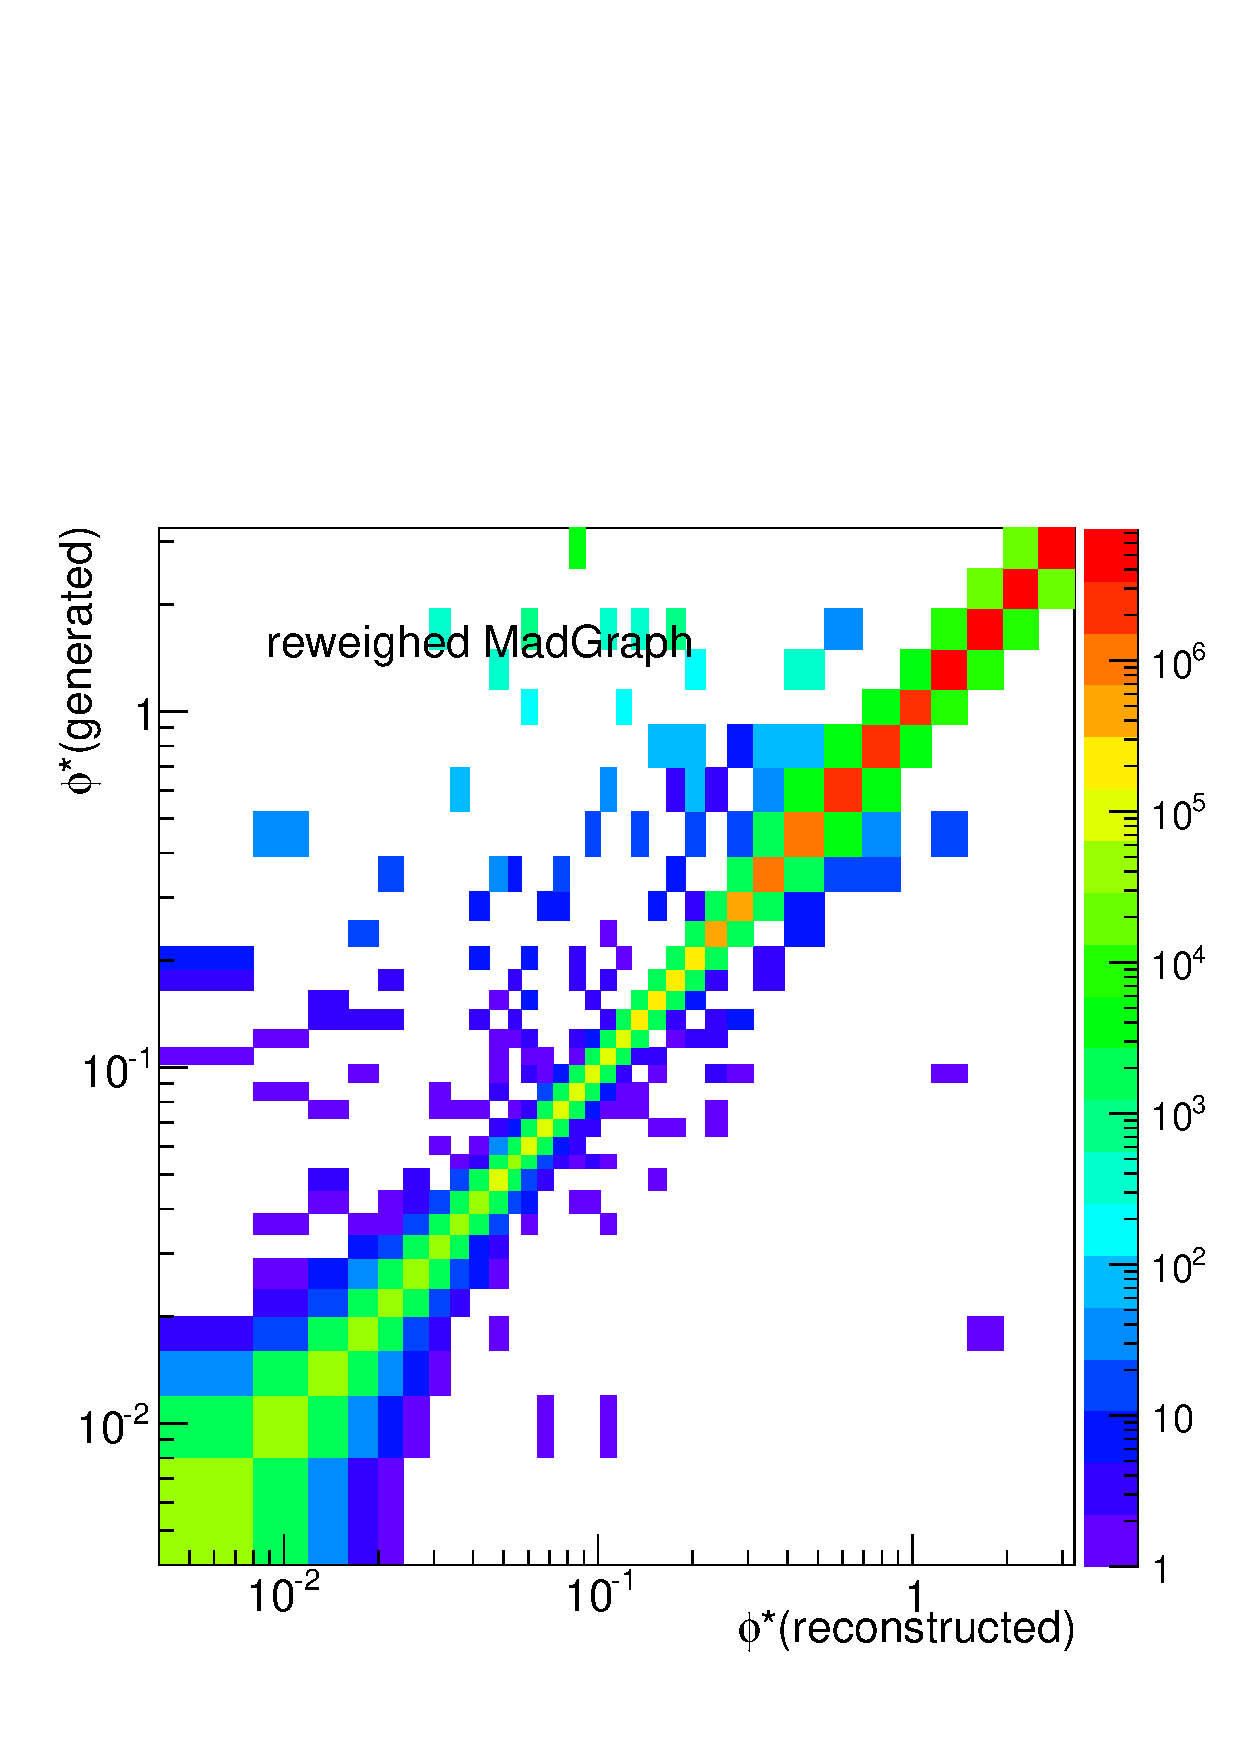
\includegraphics[width=\textwidth]{figures/BinM_M_flat.pdf}
        \caption{}
        \label{fig:unfolding_flat_bin_migration}
    \end{subfigure}
    \caption{
        The ratio between the unfolded reconstructed \phistar distribution and
        the true generated \phistar distribution for \Ztoee events generated
        with \POWHEG is shown on the left. The unfolding was done with the
        \MADGRAPH sample in which all events were reweighed inversely
        proportional to generated \phistar distribution. The bin migration
        matrix for the reweighed \MADGRAPH sample is shown on the right.
    }
    \label{fig:flat_unfolding}
\end{figure}

Differences in the resolution can arises due to differences in how the
detector is simulated and how the detector responds in reality. Various
corrections are applied to the MC in order to make it more closely match the
data; these are discussed in \SEC~\ref{sec:scale_factors}. The uncertainties
from these corrections are discussed in \SEC~\ref{sec:uncertainties}.

\subsection{Efficiency Correction}
\label{ssec:eff_correction}

Not every event which should be detected by CMS is. Some events are lost at
each stage of event selection and reconstruction. These lost events must be
corrected for in order to accurately compare our results to theory. We
therefore apply corrections for the reconstruction efficiency, the electron ID
efficiency, and the trigger efficiency.

The efficiency corrections are applied after the bin migration corrections. The
correction factors are derived for each \phistar bin using the \Ztoee \MADGRAPH
sample discussed in \SEC~\ref{ssec:monte_carlo}. Two sets of events are
selected. The first set, the ``acceptance set'', is created by applying the
acceptance definition discussed in \SEC~\ref{sec:acceptance} to the generator
level quantities in the MC. The second set, the ``final selection set'', is
created by selecting MC events by applying the full analysis selection to the
reconstructed level quantities in the MC. The efficiency in each \phistar bin
is calculated by counting the number of events in the ``final selection set''
in a bin, and dividing by the number of events in the same bin in the
``acceptance set''. This gives us an average efficiency composed of all the
efficiencies of the events in the bin. The main advantage of using this average
efficiency instead of correcting each event's efficiency individually is that
any correlations between the various efficiencies are automatically taken into
account in this process. The average efficiencies in each bin as calculated with
both \MADGRAPH and \POWHEG are shown in \FIG~\ref{fig:average_efficiencies}.

\begin{figure}[!htbp]
    \centering
    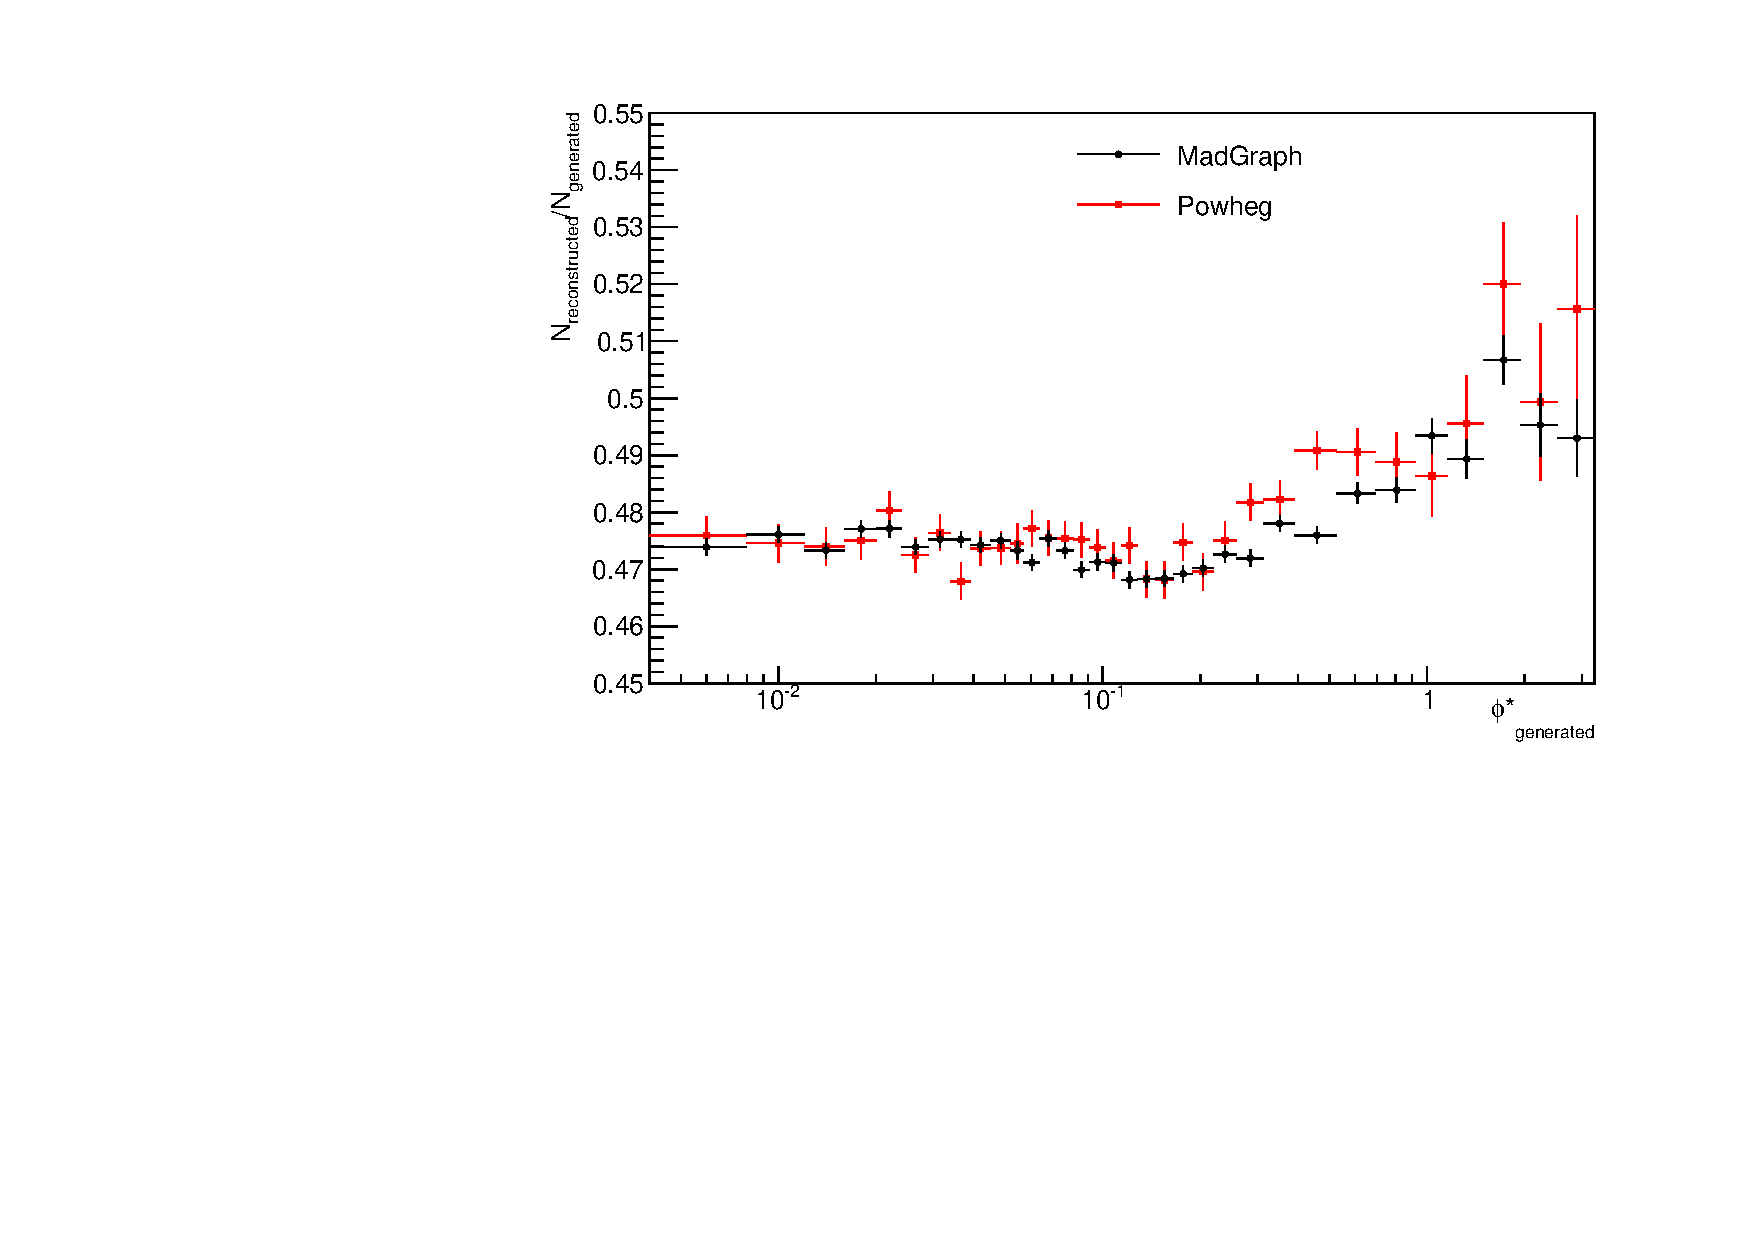
\includegraphics[width=\textwidth]{figures/EventEff.pdf}
    \caption{
        The ratio of \Ztoee events generated with \MADGRAPH (circles) and
        \POWHEG (squares) which pass our event selection over the number of
        events in our fiducial region as a function of the generated \phistar.
    }
    \label{fig:average_efficiencies}
\end{figure}
